%% An Introduction to LaTeX Thesis Template of Wuhan University
%%
%% Created by WHUTUG

\documentclass[type = bachelor]{whu-thesis}
\whusetup
  {
    info               =
      {
        title          = {金刚石氮-空位色心的\\电荷态调控和性质表征},
        title*         = {Modulation of Charge States and Characterization of Properties\\ in Nitrogen-Vacancy Centers of Diamond},
        student-number = {2020302192129},
        school         = {弘毅学堂},
        author         = {邹迪玮},
        author*        = {Diwei Zou},
        subject        = {学科},
        major          = {微电子科学与工程},
        advisor        = {周利 , 副教授;孙启超 , 研究员},
        direction      = {研究方向},
        date           = {2024/5},
        keywords       = {关键词 1 , 关键词 2 , 关键词 3 , 关键词 4 , 一个非常非常,非常非常长——的关键词 5},
        keywords*      = {key word 1 , key word 2 , key word 3 , key word 4 , {and a very very, very very long key word---the key word 5}},
      },
    style              =
      {
        graphics-path  = {{figures/}{data/}},
        list-of-figures,
        list-of-tables,
      },
    element            =
      {
        innovation     = {pages/innovation},
        abstract       = {pages/abstract},
        abstract*      = {pages/enabstract},
        bibliography   = {ref/refs , ref/thu},
        achievements   = {pages/achievements},
        thanks         = {pages/thanks},
        appendix       = {pages/appendix}
      }
  }

\begin{document}
%%----------- 主体部分 ----------- %%
\documentclass[type = bachelor]{whu-thesis}
\usepackage{textcomp,mathcomp}
\usepackage{siunitx}
\usepackage{chemfig}
\usepackage{graphicx}

\whusetup
  {
    info               =
      {
        title          = {金刚石氮-空位色心的\\电荷态调控和性质表征},
        title*         = {Modulation of Charge States and Characterization of Properties\\ in Nitrogen-Vacancy Centers of Diamond},
        student-number = {2020302192129},
        school         = {弘毅学堂},
        author         = {邹迪玮},
        author*        = {Diwei Zou},
        subject        = {学科},
        major          = {微电子科学与工程},
        advisor        = {周利 , 副教授;孙启超 , 研究员},
        direction      = {研究方向},
        date           = {2024/5},
        keywords       = {关键词 1 , 关键词 2 , 关键词 3 , 关键词 4 , 一个非常非常,非常非常长——的关键词 5},
        keywords*      = {key word 1 , key word 2 , key word 3 , key word 4 , {and a very very, very very long key word---the key word 5}},
      },
    style              =
      {
        graphics-path  = {{figures/}{data/}},
        list-of-figures,
        list-of-tables,
      },
    element            =
      {
        innovation     = {pages/innovation},
        abstract       = {pages/abstract},
        abstract*      = {pages/enabstract},
        bibliography   = {ref/refs_1}
      }
  }
\begin{document}

% Chapter 1

\chapter{金刚石中的氮-空位色心(NV Center)}

\section{金刚石材料}
金刚石是碳元素的一种常见的同素异形体,在晶体结构上,每一个碳原子被周围的四个碳原子包围并与之形成共价键,从而形成四面体的面心立方结构的晶体。金刚石中的碳原子紧密结合在一起,这样特殊的晶体结构和原子之间稳定的键合方式使得金刚石拥有很多物理和化学上的优异性质,如高硬度、高热导率、高折射率、高抗压强度、高化学稳定性、高电阻率、低热膨胀系数、低摩擦系数、低表面粗糙度、低吸附性等。这些优异的性质使得金刚石在很多领域都有着广泛的应用,如磨料、切割工具、磨料涂层、磁头、光学窗口、高功率激光器件、高频电子器件、生物医学器件等。

金刚石是最坚硬的天然形成的物质,其机械硬度高达 10000 \unit{\kilogram\per\milli\meter\squared},德拜温度高达1860 \unit{\kelvin},它的杨氏模量为1050 \unit{\GPa},有着22 \unit{\watt\per\centi\meter\per\kelvin}的热导率、较低的热展宽系数、较高的击穿电场强度(> 10 \unit{\mega\volt\per\centi\meter}),以及较强的载流子迁移率(对于电子为4500 \unit{\centi\meter\squared\per\volt},对于空穴为3800 \unit{\centi\meter\squared\per\volt})。对于纯净的金刚石而言,其密度为$\rho =$ 3.52 \unit{\g\per\cm},折射率$n =$ 2.39,同时有5.47 \unit{\electronvolt}的较宽带隙,这使其投射光谱范围非常广,从紫外波段(Ultraviolet, UV)到近红外波段(Near Infrared, IR)都可以覆盖到,外观高度透明纯净,拥有极高的透光率 \cite{mildren2013optical, lonvcar2013quantum}。

金刚石在结构上的稳定性使得其化学性质非常的不活跃,因此它几乎不能和大部分化学物质发生反应。所以金刚石有着极低的细胞毒性,使得其在生物、医学领域有着广泛的应用 \cite{schirhagl2014nitrogen,wu2016diamond}。同时,金刚石的化学稳定性也使得其在高温、高压、强腐蚀性环境下有着很好的稳定性,因此金刚石也被广泛应用于高温、高压、强腐蚀性环境下的传感器、探测器等器件中 \cite{umezawa2012high, jayaraman1983diamond}。

由于金刚石晶体的结构非常的整齐和规则,在自然情况下,只有很少一部分的杂质会存在于金刚石晶体中,并参与形成晶格结构。自然界中常见的最主要的金刚石中的杂质是氮和硼元素,因此金刚石可以根据杂质的种类和含量分为不同的类型,主要有两种大类:type \uppercase\expandafter{\romannumeral1}和type \uppercase\expandafter{\romannumeral2},在其中又可以分为四个子类:type \uppercase\expandafter{\romannumeral1}a、type \uppercase\expandafter{\romannumeral1}b、type \uppercase\expandafter{\romannumeral2}a、type \uppercase\expandafter{\romannumeral2}b \cite{breeding2009type}。在这些分类中,type \uppercase\expandafter{\romannumeral1}型的金刚石中主要含有氮元素杂质,type \uppercase\expandafter{\romannumeral1}a型金刚石中的氮元素含量较高,最多有3000 ppm(parts per million,即百万分之一);而type \uppercase\expandafter{\romannumeral1}b型金刚石中的氮元素含量稍低,一般情况下不到500 ppm。由于空气中广泛存在的氮气和土壤中各种各样的氮元素,在自然界中形成的金刚石通常为type \uppercase\expandafter{\romannumeral1}a或者\uppercase\expandafter{\romannumeral1}b。对于type \uppercase\expandafter{\romannumeral2}型的金刚石而言,氮元素的含量远远小于type \uppercase\expandafter{\romannumeral1}型金刚石,通常低于20 ppm。其中,type \uppercase\expandafter{\romannumeral2}b型金刚石中的硼元素杂质含量要高于type \uppercase\expandafter{\romannumeral2}a型。Type \uppercase\expandafter{\romannumeral2}型金刚石的含量极其稀少,而且很少能在自然界中被发现。在科学研究中,type \uppercase\expandafter{\romannumeral2}型金刚石由于其晶体纯净的性质,有着各种各样独特的应用场景。对于科学研究而言,为了保证金刚石样品性质的一致性和实验的可重复性,高纯度和可控掺杂的人造金刚石生长合成技术应运而生 \cite{sumiya1997crystalline, spitsyn1981vapor, gracio2010diamond}。

\subsection{人工合成生长金刚石}
目前主流的人造金刚石样品合成技术主要分为两种,一种是高温高压方法(High Pressure High Temperature,HPHT)和化学气相沉积法(Chemical Vapor Deposition, CVD)。对于HPHT方法而言,其原理主要是模仿天然金刚石在地壳中的形成过程,将碳元素另一种常见的同素异形体石墨的晶体结构在极端的超高温超高压环境下(温度在\SI{1400}{\degreeCelsius}左右,压强在\SI{5.5}{\GPa}左右),通过金属触媒粉的催化作用,转换成具有$sp^3$杂化轨道的金刚石晶体结构 \cite{dossa2023analysis}。HPHT方法使得人类可以在工业上大规模高效率地生产type \uppercase\expandafter{\romannumeral1}型金刚石,但是由于空气中大量的氮气存在,HPHT方法难以生产高纯度低杂质含量的type \uppercase\expandafter{\romannumeral2}型金刚石。由此,为了制备高纯度和可控掺杂的实验级金刚石样品,化学气相沉积的方法逐渐受到科学家们的关注和广泛使用。

CVD方法是一种铜质外延的生长过程,需要在金刚石晶种基面上生长新的金刚石\cite{isberg2002high,isberg2002high}。因此,对于生长出来的晶体,其质量主要取决于晶种的种类和取向,而在非金刚石晶种表面生长会导致生长出有许多单晶金刚石各向同性紧密结合形成的多晶金刚石晶体\cite{mildren2013optical, jahnke2012long}。如果想要形成科学实验中可用的单晶金刚石,就必须用单晶金刚石作为晶种来进行CVD生长。在实际生长的过程中,科学家们通常用{100}取向的晶种衬底来保证尽可能少的生长缺陷\cite{gicquel2001cvd}。

在CVD方法生长金刚石的过程中,除了晶种之外,碳元素源也是比较重要的一个因素。通常情况下,碳元素主要来自于烃类气体,甲烷\chemfig{CH_4}和氢气\chemfig{H_2}的混合气体就是在实验合成的过程中较为理想易得的碳源。对于CVD生长金刚石的过程而言,这些碳源气体需要通过不同的方法来激活,常见的方法有通过热丝(hot filament)或者微波等离子体(microwave plasma),其中微波等离子体气相沉积(Microwave Plasma Chemical Deposition, MPCVD)的方法是生长type \uppercase\expandafter{\romannumeral2}型金刚石最有效的方法\cite{robins1990line, nemanich2014cvd}。在微波等离子体激活后,碳源气体内部形成许多高度反应性的自由基(reactive radicals),活跃的氢自由基(H$\cdot$)有两个重要的功能,一个是终止了已经生长的金刚石表面,从而防止具有$sp^2$杂化轨道的石墨碳原子;其次氢原子可以刻蚀掉已经生成的具有$sp^2$杂化轨道的石墨碳原子,从而在晶种沉底表面上提供悬垂的$sp^3$化学键,使其能够和已经极化的甲基自由基(CH$_3\cdot$)轻松结合,使得单晶金刚石能在沉底表面逐渐生长\cite{denisenko2010surface}。在生长的过程中,各种参数同样十分重要,例如生长腔内压强、温度、气体流速、微波功率等因素决定了生长出来的金刚石的各种性质,使其适用于不同的应用场景。本人于2021年的时候提出了一种n型共掺杂金刚石半导体材料制备的多尺度耦合仿真方法,通过宏观-介观-微观三个尺度的相互耦合,调整MPCVD方法生长金刚石过程中的各种参数,来提高特定用途金刚石的生长合成效率\cite{CN113096749B}。

\subsection{金刚石晶体结构}
金刚石晶体是由每个碳原子和周围四个相邻的碳原子结合,生成四个共价键组成的正四面体结构,其晶格常数为$a_0 = 3.567$ \unit{\angstrom}。金刚石晶体可以看成是两个面心立方晶体的嵌套,其中一个面心立方晶体在三维空间的三个轴上上相对于另一个移动了$\frac{a_0}{4}$,原点从$(0, 0, 0)$移动到了$(\frac{a_0}{4}, \frac{a_0}{4}, \frac{a_0}{4})$。这样的晶体结构使得金刚石非常的坚硬,每一个晶胞中包含着8个碳原子,每一个碳原子的核外电子都呈现$sp^3$杂化轨道结构,和相邻的四个碳原子形成长度为1.44 \unit{\angstrom}的共价键,它的晶体结构见图 \ref{fig: Diamond Lattice}所示。

\begin{figure}[h]
  \centering
  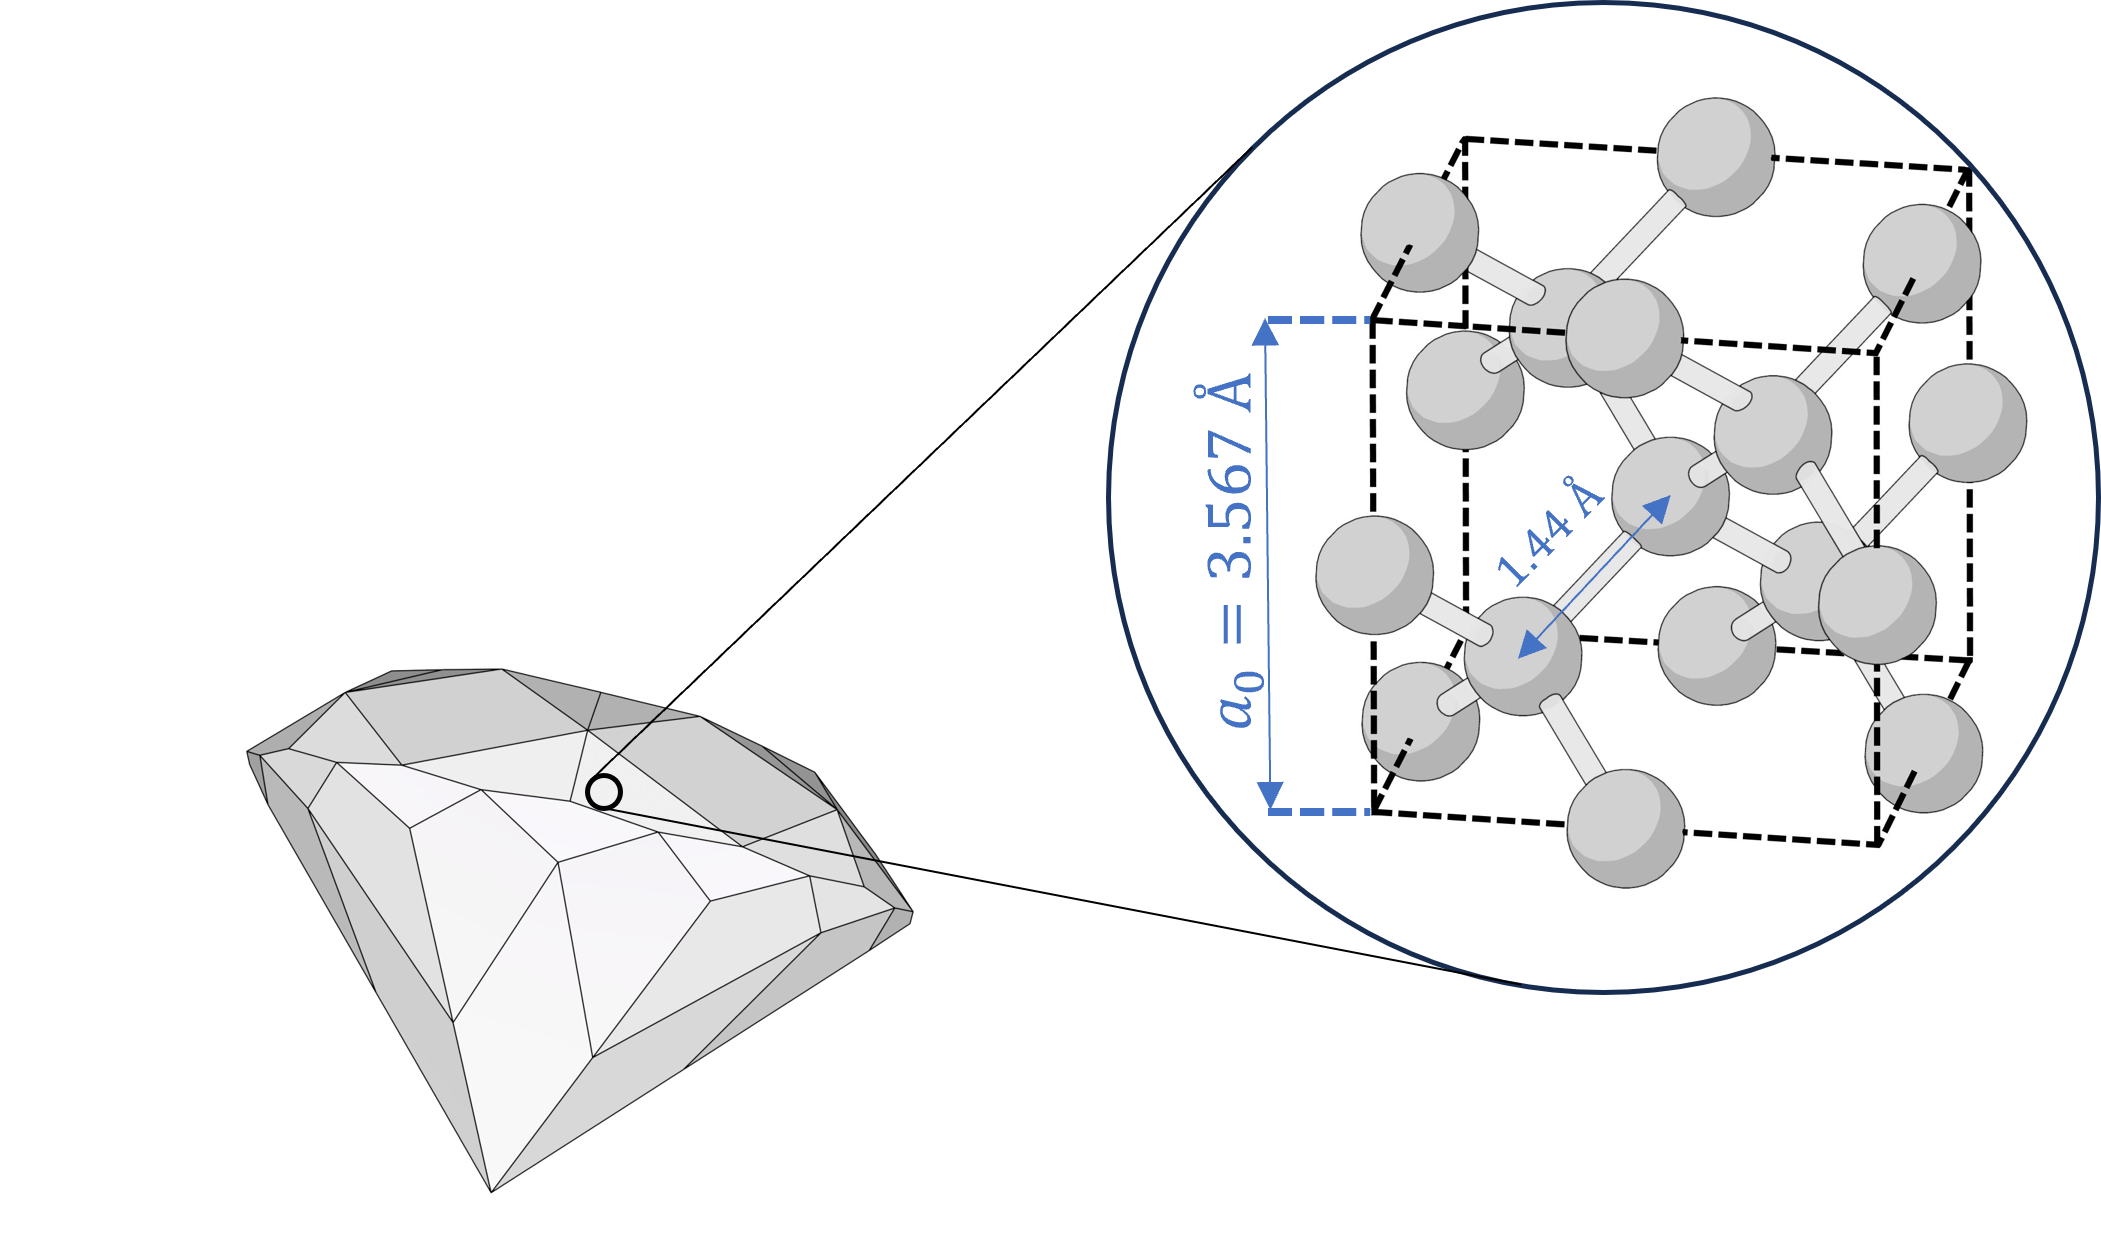
\includegraphics[width=0.9\textwidth]{figures/Chapter 1/Diamond Lattice.png}
  \caption[金刚石及其晶胞结构]{金刚石及其晶胞结构\cite{staudacher2015nuclear}}
  \label{fig: Diamond Lattice}
\end{figure}

然而,在金刚石晶体合成或生长的过程中,晶格缺陷会不可避免的出现,它们会对金刚石的性质产生各种各样的影响,尤其是电子结构产生较大的影响\cite{jelezko2006single, nebel2003electronic}。金刚石晶体中最常见的晶格缺陷是空位(vacancy),这是一种本征晶格缺陷,源于金刚石的中的单个碳原子在其原本的晶格结构上的缺失,每一个孤立的空位可以吸收741 nm的光子,有着高浓度空位的金刚石在一定条件下会呈现蓝绿色的色调,因此金刚石晶体结构中的空位缺陷也被称为色心(color centers),如图 \ref{fig: Color Center}所示\cite{waldermann2007creating, kiflawi2007electron}。

\begin{figure}
  \centering
  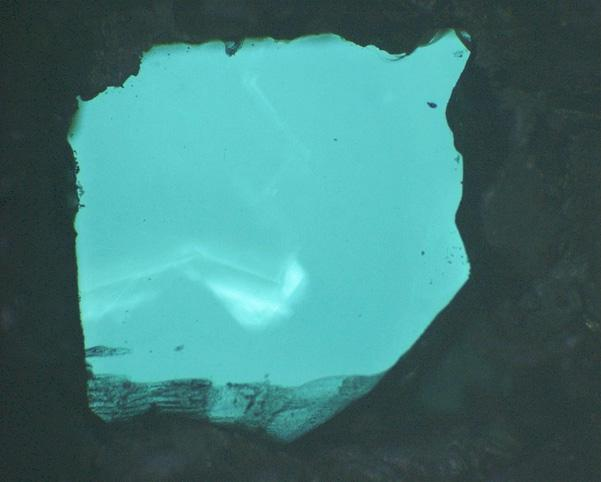
\includegraphics[width=0.7\textwidth]{figures/Chapter 1/Color Center.jpg}
  \caption[电子辐照的type \uppercase\expandafter{\romannumeral1}a型金刚石样品显微图片]{电子辐照的type \uppercase\expandafter{\romannumeral1}a型金刚石样品显微图片。浅色区域的空位和氮浓度较低,样品尺寸为\(1\times1\times0.5 \, \mathrm{mm^3}\) \cite{kiflawi2007electron}。}
  \label{fig: Color Center}
\end{figure}

\subsection{金刚石中的色心}
金刚石是一种宽禁带半导体,实验上测得其价带(valence band,VB)和导带(conduction band,CB)之间的带隙宽度大约为5.5 \unit{\eV} \cite{mildren2013optical,cheng2023bandgap,wort2008diamond}。尽管纯净的金刚石呈现无色透明的质地,可以透过的波长范围从UV到IR,但是由于晶格中存在的缺陷或者杂质,使得金刚石体系的带隙之中会出现额外的能级结构,其中的一些能级结构具有活跃的光学性质。因此,这些缺陷结构可以吸收可见光,并在缺陷浓度足够高的时候,使得金刚石材料呈现出特定的颜色,比如高浓度的硼元素会使金刚石呈现蓝色,镍元素相关的缺陷会让金刚石呈现棕色。目前人类已知金刚石中的涉及到光学跃迁性质的荧光缺陷有超过100种,这些缺陷都可以被称为色心\cite{koizumi2008physics,jelezko2006single}。许多的色心都和氮元素杂质有关,因为氮元素是金刚石中最常见的元素,高浓度的氮元素掺杂会使得金刚石呈现黄色的色泽\cite{breeding2020naturally, zaitsev2016spectroscopic}。

金刚石色心种的缺陷能级和电子结构之间的光学跃迁过程可以被人为地进行激光调控,在这个过程中会有不同的激发机理,取决于色心相关的缺陷能级的性质,如图 \ref{fig: Optical Transition}所示。比如,激光的光子可以将缺陷能级的电子激发到导带之中(见图 \ref{fig: Optical Transition}a \uppercase\expandafter{\romannumeral1}所示),或者将电子从夹带激发到缺陷能级见图 \ref{fig: Optical Transition}a \uppercase\expandafter{\romannumeral2所示}。另一种常见的情况是在带隙中有多个缺陷能级的情况,激光可以将电子从一个缺陷能级激发到另一个缺陷能级(见图 \ref{fig: Optical Transition}b所示),这种跃迁的方式相较于电子在缺陷能级和导带(或价带)之间相互跃迁能为高效和可控\cite{gali2011time,gali2012excitation}。在各种各样的色心之中,氮-空位色心(Nitrogen-Vacancy Center)在近些年来被许多科学家所广泛研究,其在532 nm激光的激发下会发出红色的荧光,以此为特征对它的性质进行观测和表征\cite{doherty2013nitrogen}。

\begin{figure}
  \centering
  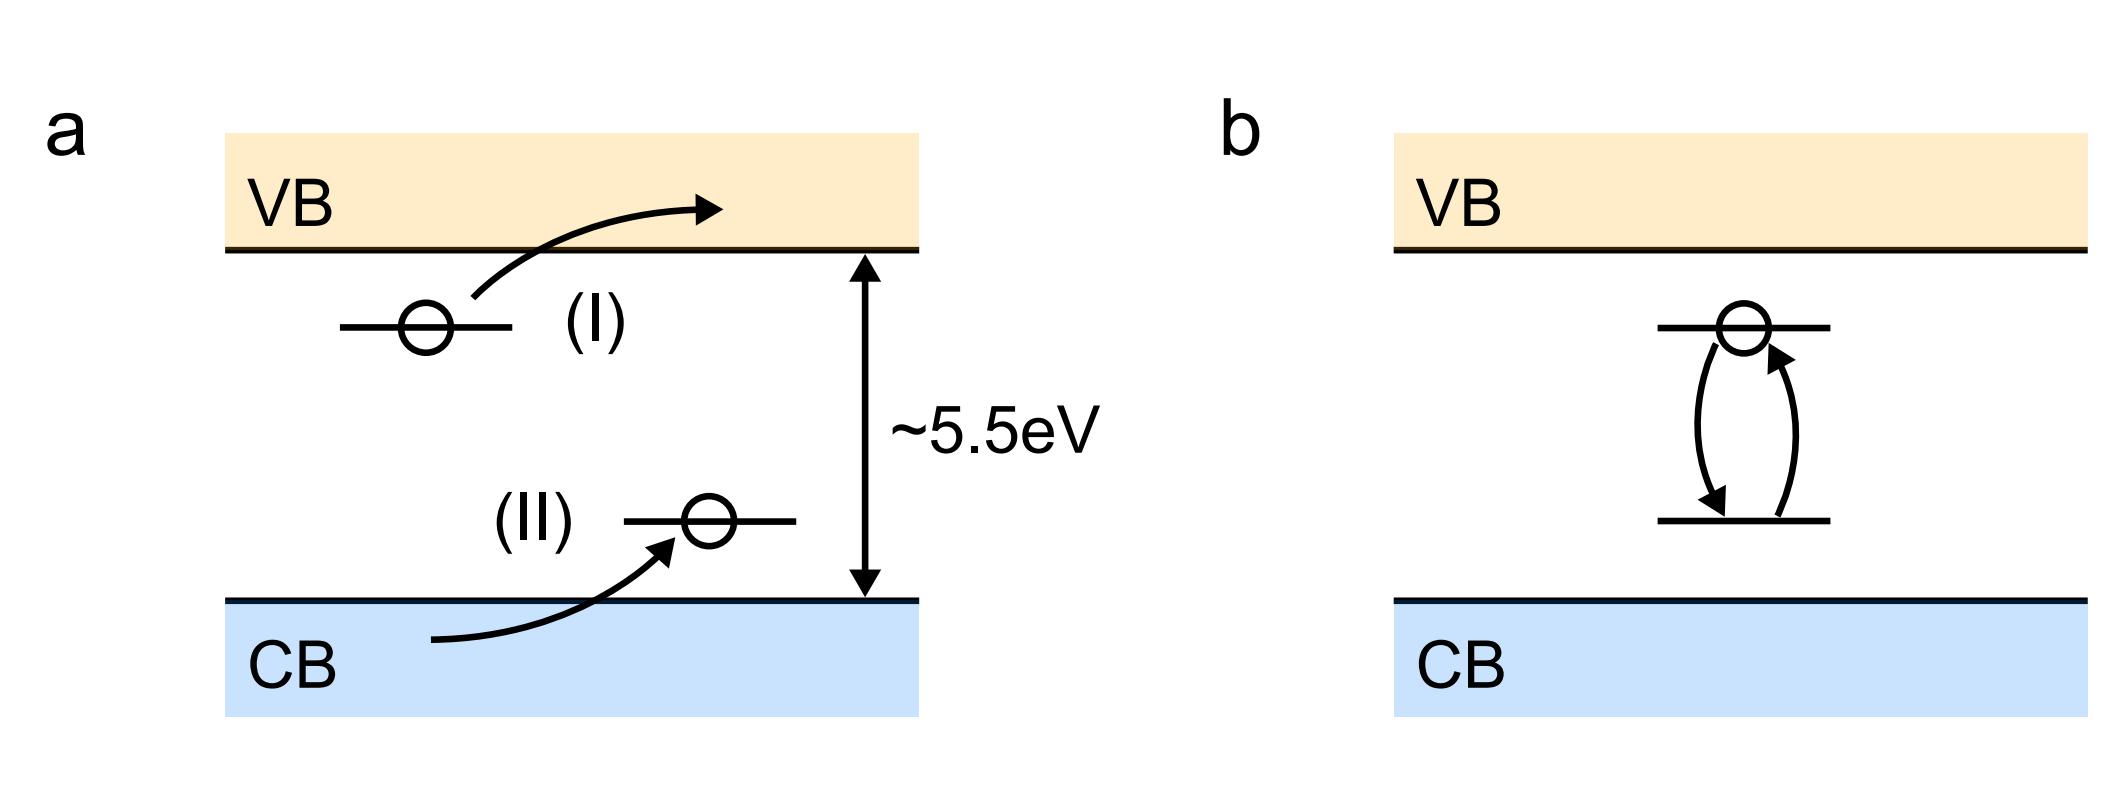
\includegraphics[width=0.9\textwidth]{figures/Chapter 1/Optical Transition.png}
  \caption[含有缺陷的金刚石晶体的电子能级结构]{含有缺陷的金刚石晶体的电子能级结构。(a)带隙之间的施主和受主能级会使电子发生在价带和缺陷能级(\uppercase\expandafter{\romannumeral1})或缺陷能级和导带(\uppercase\expandafter{\romannumeral2})之间的光学跃迁。(b)电子在施主和受主能级之间的光学跃迁\cite{staudacher2015nuclear}。}
  \label{fig: Optical Transition}
\end{figure}

\section{NV Center的结构和性质}

由于本文主要是围绕金刚石中氮-空位色心的各种性质进行讨论,并结合实验对其进行表征,因此本节将对其结构和性质进行详细的介绍。氮-空位色心不仅仅存在于金刚石中,还可能存在于其他的半导体晶体如碳化硅(SiC)之中,而本文所有的讨论和实验都是基于金刚石中的氮-空位色心,出于方便起见,后文叙述中所有的“NV色心”和“NV Center”都是指金刚石中的氮-空位色心\cite{von2015identification, csore2017characterization}。

\subsection{NV Center的晶体结构}
NV Center是金刚石中最常见的色心之一,其结构如图 \ref{fig: NV Structure}所示,它是由一个氮原子替位原本的碳原子和邻近的一个空位缺陷组成的复合缺陷结构,其晶格结构中的空位缺陷是金刚石晶格中最常见的缺陷,而氮原子是金刚石中最常见的杂质之一,因此NV Center是金刚石中最常见的色心之一。我们定义NV Center的轴向为氮原子和空位中心的连线,也就是晶胞的[111]轴向。氮原子和围绕空位的三个碳原子形成了高度对称的$C_{3v}$对称性结构,这种结构使得NV Center的晶体结构具有很高的对称性(其结构对称性见图 \ref{fig: NV Symmetry}),从而使得NVCenter的电子结构和光学性质具有很高的稳定性。

\begin{figure}
  \centering
  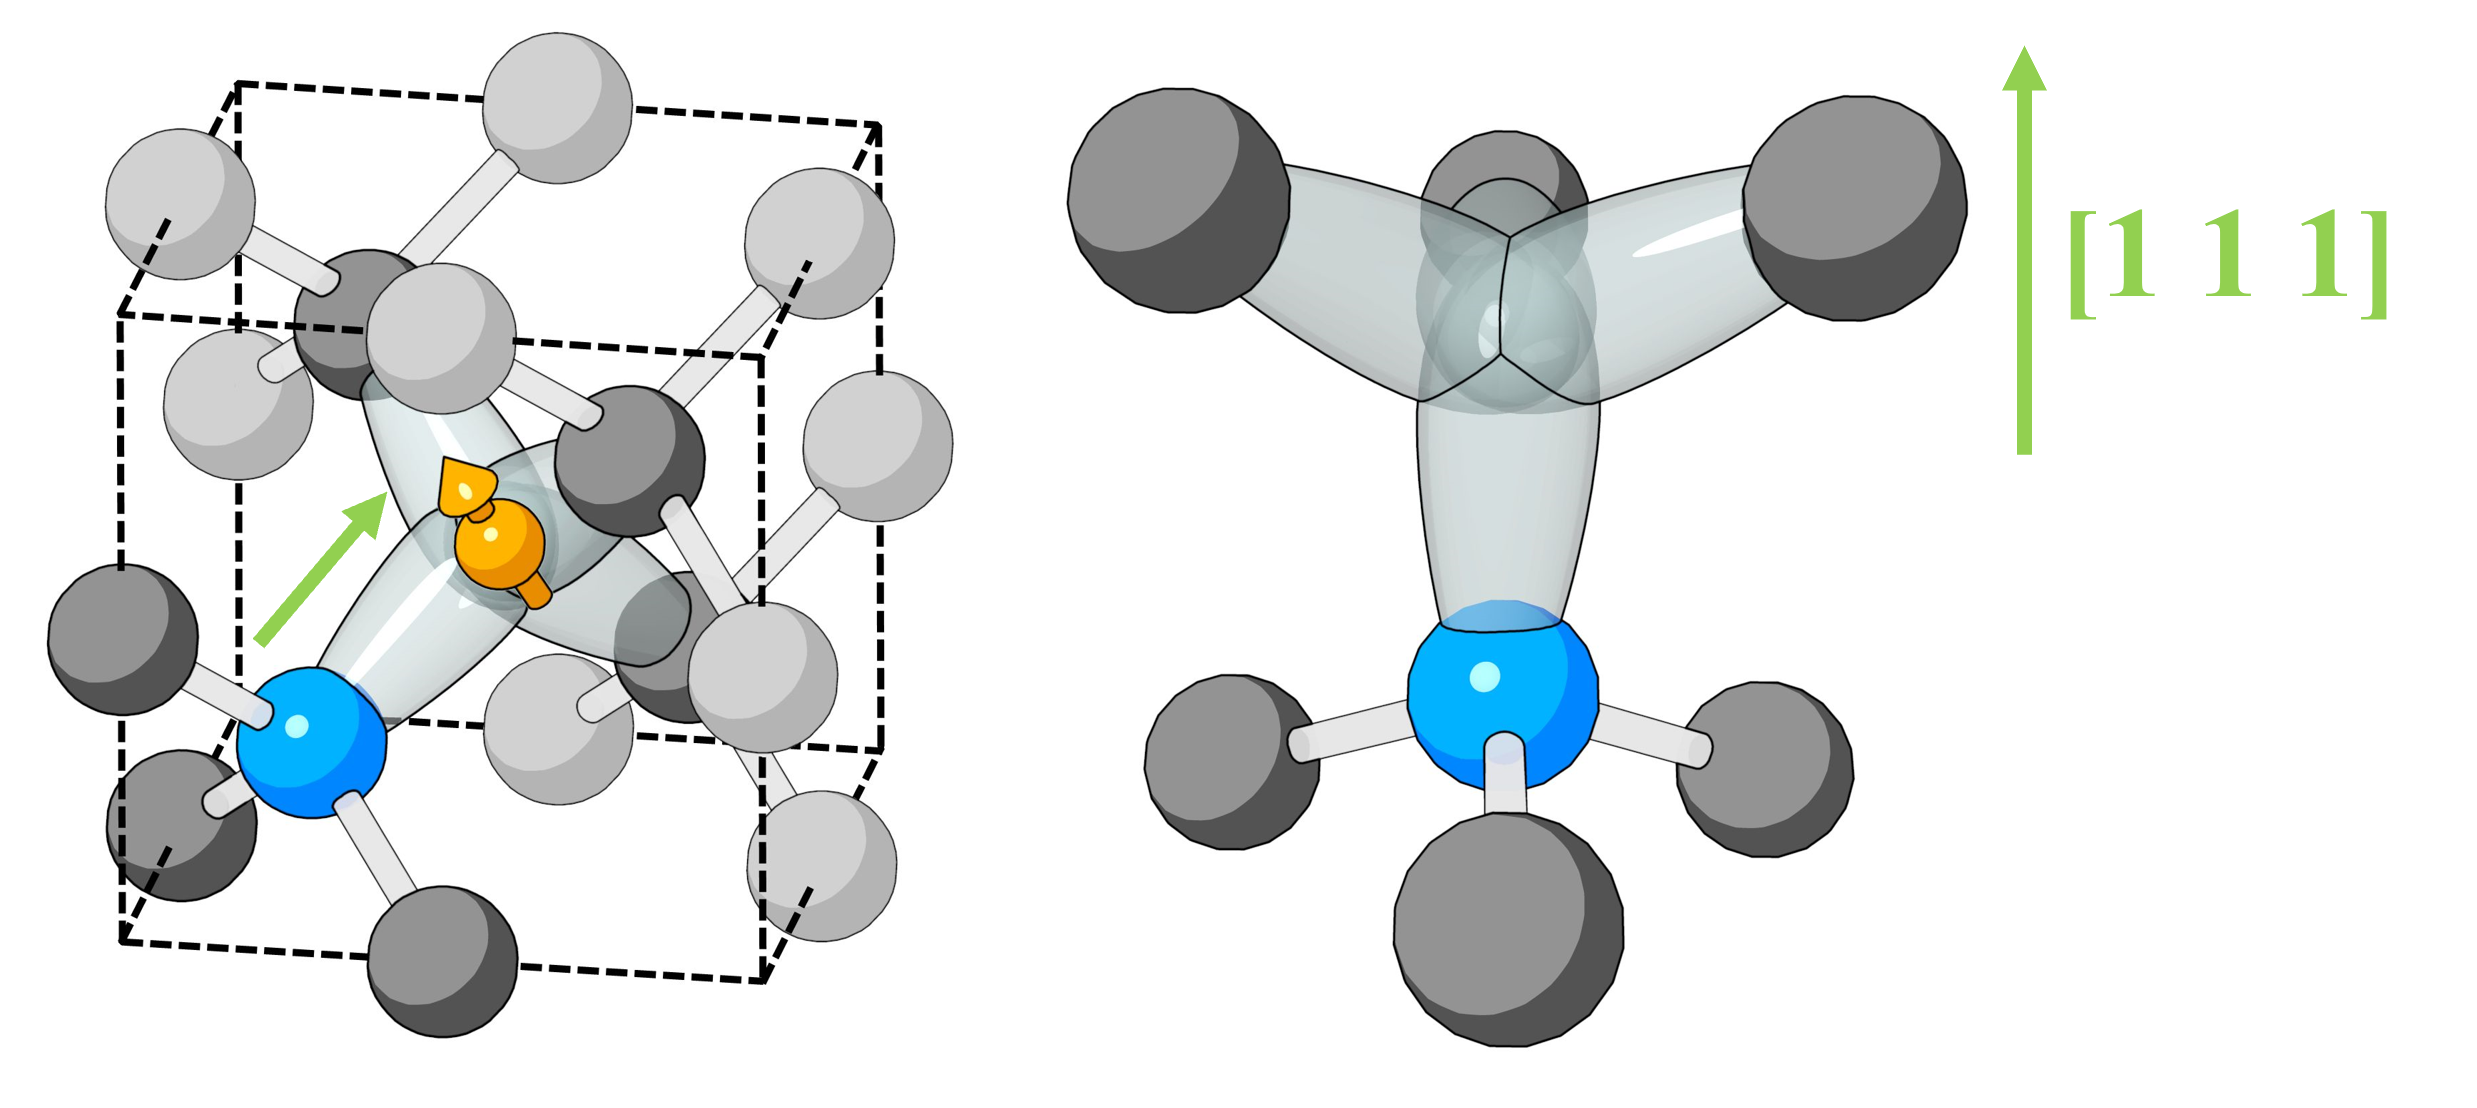
\includegraphics[width=0.9\textwidth]{figures/Chapter 1/NV Structure.png}
  \caption[金刚石中NV Center的结构]{金刚石中NV Center的结构,其中深蓝色的原子为氮原子,橙色的电子自旋标识符处为空位,围绕在NV Center周围的碳原子为深灰色\cite{staudacher2015nuclear}。}
  \label{fig: NV Structure}
\end{figure}

\begin{figure}
  \centering
  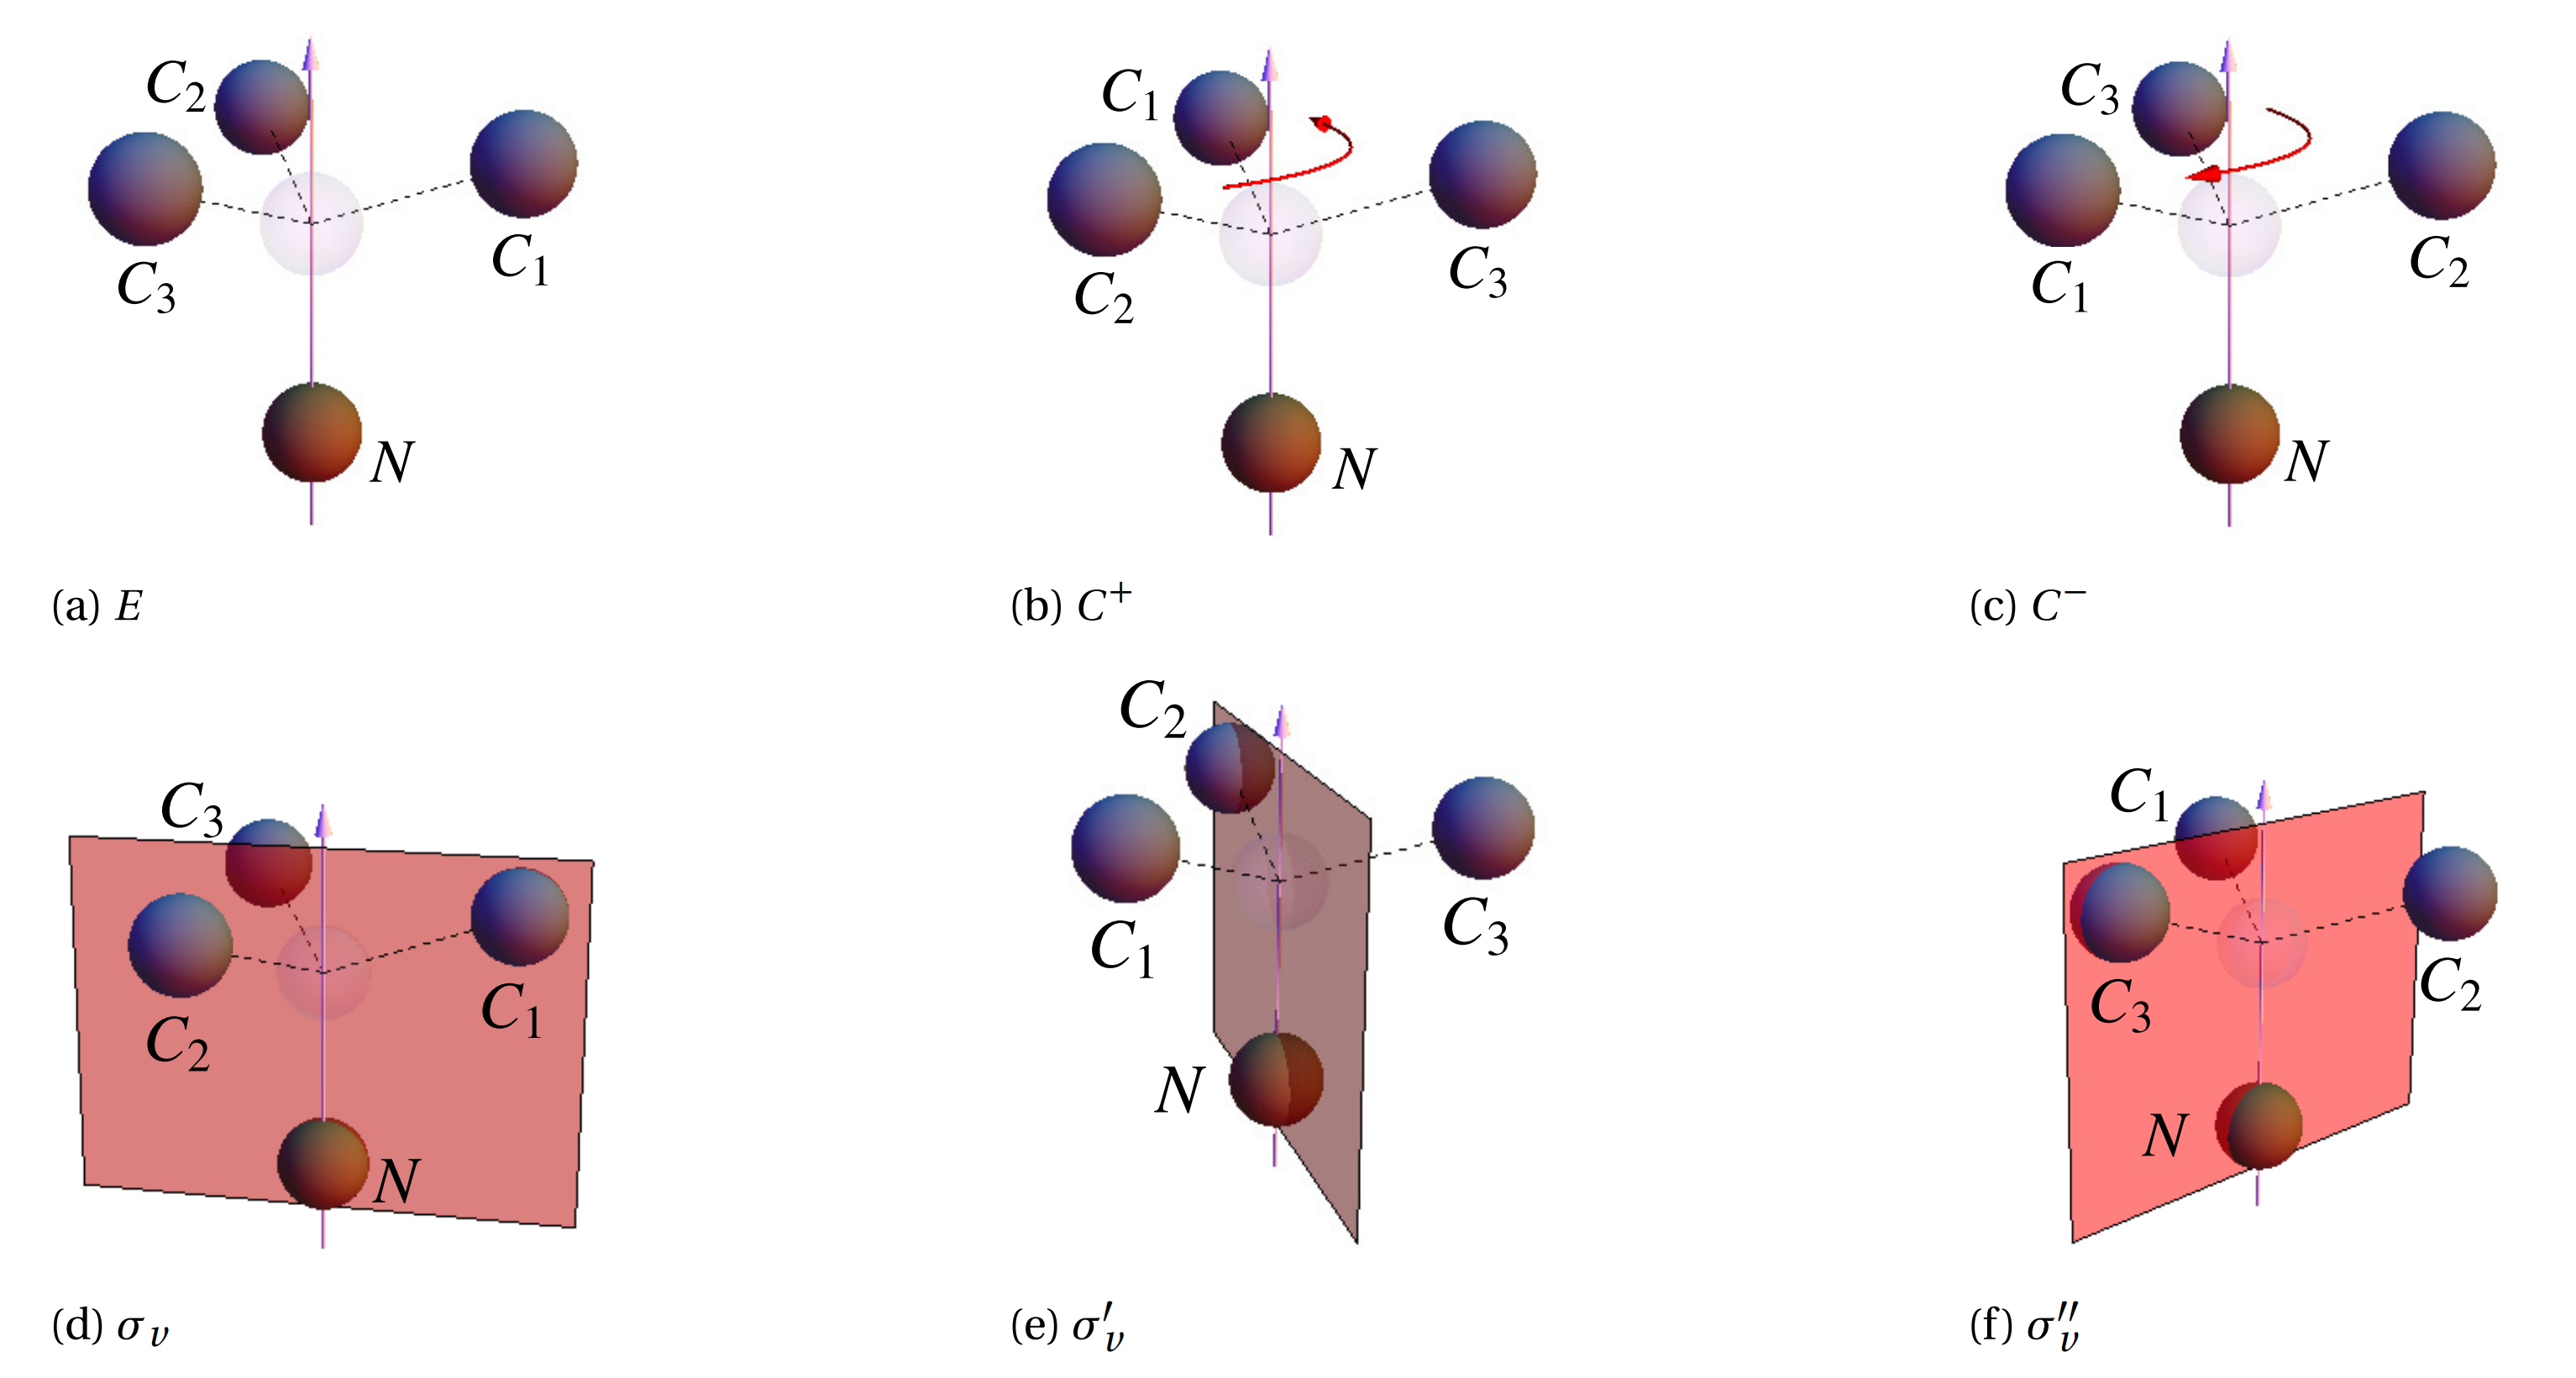
\includegraphics[width=1.0\textwidth]{figures/Chapter 1/NV Symmetry.png}
  \caption[金刚石的C$_{3v}$对称性群结构]{金刚石的C$_{3v}$对称性群结构,氮原子和围绕空位(中心半透明标识)的三个碳原子沿着[111]轴旋转对称,同时也沿着每个碳原子分别和空位、氮原子组成的平面镜像对称\cite{doherty2013nitrogen}。}
  \label{fig: NV Symmetry}
\end{figure}

近十几年来,随着半导体的工艺进步和计算机的广泛运用,人们开发了许多强有力的科学计算工具,通过基于密度泛函理论(Density Functional Theory, DFT)第一性原理(First-principles),利用杂化泛函Heyd-Scuseria-Ernzerhof (HSE06)算法可以较为准确地得到NV Center的自旋密度(Spin Density)和带隙中各能级的电荷密度(Charge Density),如图 \ref{fig: Spin and Charge Density}所示,可以看到NV$^-$的自旋密度和带隙中各个缺陷能级的电荷密度都是围绕$C_{3v}$旋转对称\cite{zou2023influence}。

\begin{figure}
  \centering
  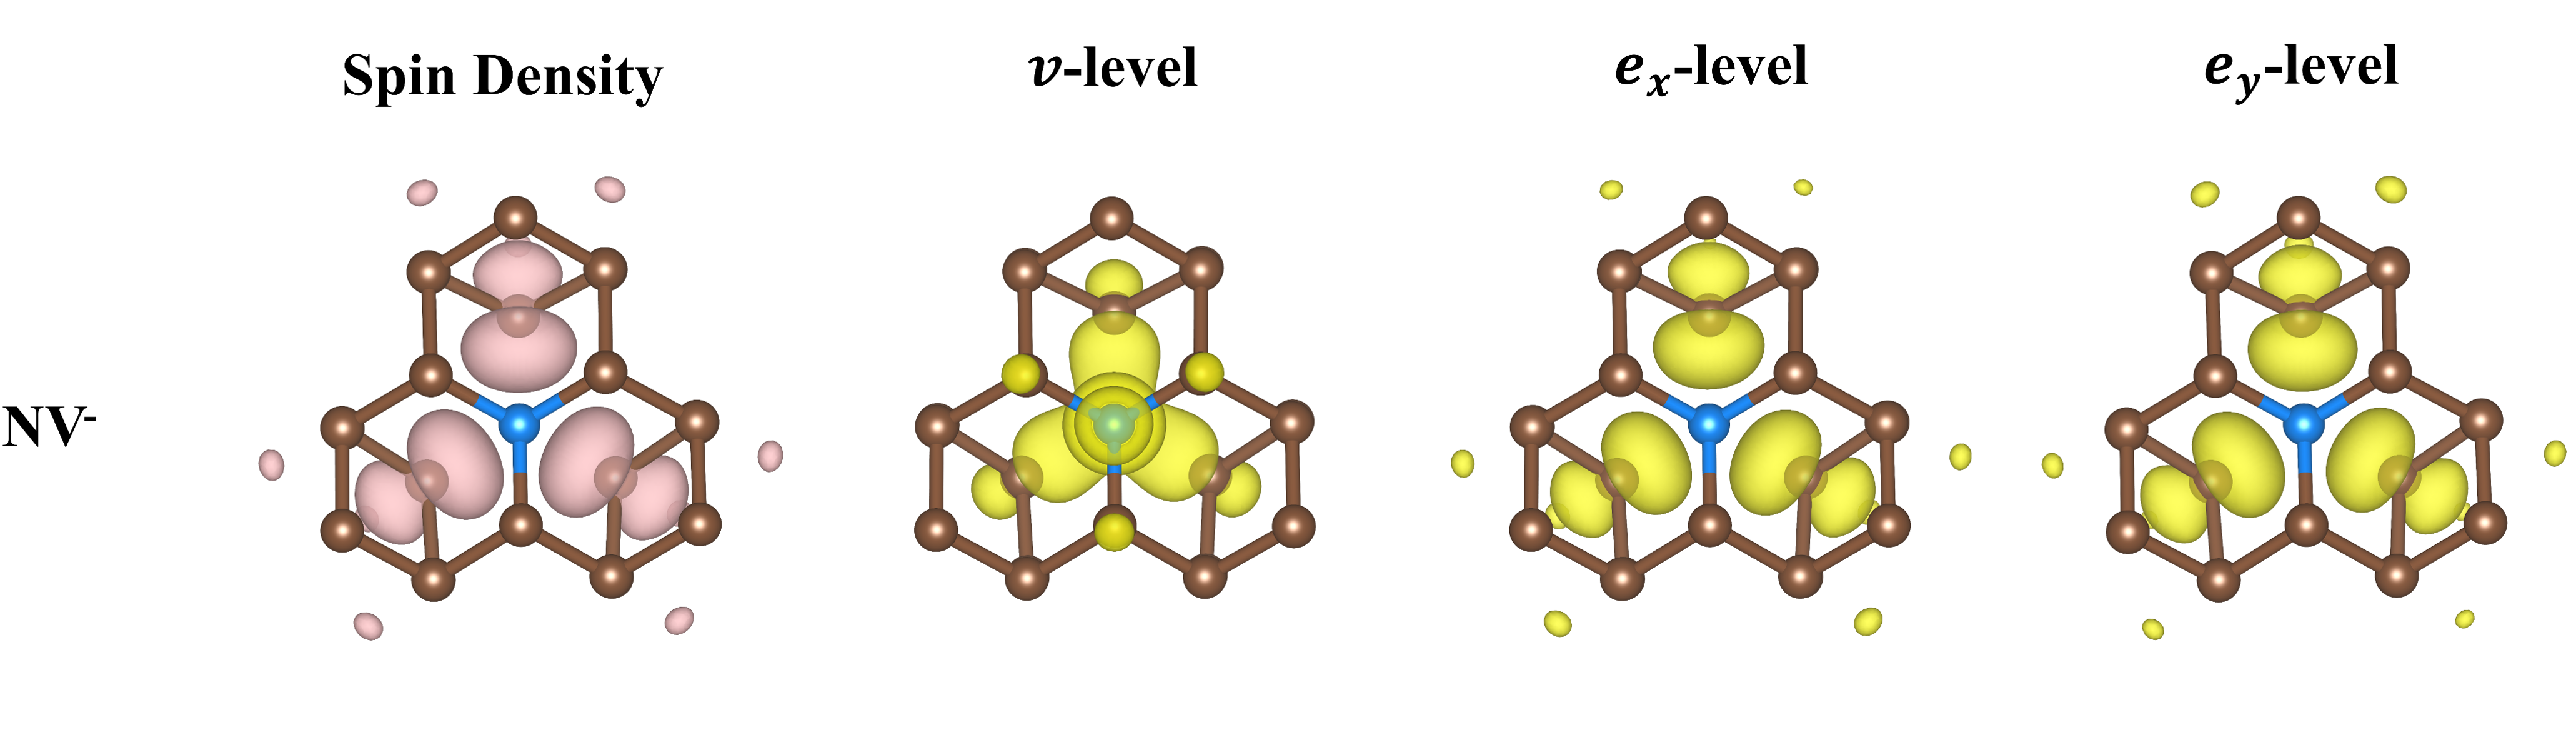
\includegraphics[width=1.0\textwidth]{figures/Chapter 1/Spin and Charge Density.png}
  \caption[基态NV$^-$的自旋密度和带隙中各个缺陷能级的电荷密度分布]{基态NV$^-$的自旋密度和带隙中各个缺陷能级的电荷密度分布,其中蓝色的原子为氮原子,棕色的原子为碳原子,视角沿$C_{3v}$轴的[-1 -1 -1]方向,粉红色的区域为自旋密度分布,淡黄色的区域为电荷密度分布,绘图参数isovalue的值设置为0.0078 \unit{e\per\bohr\cubed}\cite{zou2023influence}。}
  \label{fig: Spin and Charge Density}
\end{figure}

由于氮元素是元素周期表上第五主族的元素,所以其外围电子层中有五个价电子,其中三个电子和周围三个碳原子结合形成共价键,剩余两个电子和空位周围的三个碳原子上剩余的一个电子共五个电子形成了中性的NV CenterNV$^0$,因此五个电子形成的自旋系统有一个孤立的电子自旋,所以NV$^0$的电子自旋量子数$S=\frac{1}{2}$。在实验上已经发现的NV Center的两种稳定的电荷态,中性的NV$^0$和带负电的NV$^-$,其中NV$^-$的电子自旋量子数$S=1$ \cite{waldherr2011dark,aslam2013photo,dolde2014nanoscale}。NV Center的电荷态取决于其周围的环境状态,比如附近存在的杂质、缺陷、电场,或者周围的施主、受主能级等,更进一步地,取决于整个金刚石体系的费米能级(Fermi Level,$E_F$)\cite{doherty2013nitrogen}。在金刚石中,NV Center的电荷态可以通过光学方法进行调控,比如通过激光光子的吸收和发射,可以使NV Center的电荷态在NV$^0$和NV$^-$之间进行转换\cite{doi2016pure,siyushev2013optically,shields2015efficient}。通常情况下,NV Center可能并不会处于某种特定单一的状态,而是在两个电荷态之间不断地切换。在NV Center的电荷态切换的过程中,其电子自旋态也会发生变化,这种变化可以通过光学方法进行探测和读出,从而可以对NV Center的电荷态进行探测,这也是本文主要聚焦的问题。

对于NV Center的两种电荷态NV$^0$和NV$^-$而言,我们最主要的区分方式就是其光谱特征的不同,两种电荷态在零声子线处(zero phonon line, ZPL)都有较为强烈的光学跃迁现象。零声子线是指在光谱中的一种特殊峰值或能级跃迁,其特点是在跃迁过程中不伴随着声子(晶格振动)的吸收或发射,此状态下的能级跃迁是非常干净和锐利的,不受热振动的影响,通常情况下接近绝对零度的时候,声子的振动作用极其微弱,晶体的大部分光学跃迁都接近于ZPL的波长。零声子线通常表示了一个非常纯净的能级跃迁,因为它不受晶格振动引起的能级展宽的影响。如图 \ref{fig: NV Spectrum}所示,NV$^-$的零声子线位于637 nm处,而NV$^0$的零声子线位于575 nm处。在室温条件下,由于声子振动不可避免的影响,零声子线总会伴随着较强的声子边带(phonon sidebands, PSB)效应,导致NV Center的光谱出现展宽现象,而不是在ZPL处出现极其尖锐突出的峰值。

\begin{figure}
  \centering
  \includegraphics[width=1.0\textwidth]{figures/Chapter 1/NV Spectrum.png}
  \caption[NV Center在不同电荷态的时候的光谱图象]{NV Center在不同电荷态的时候的光谱图象,其中红色的线为NV$^-$的光谱,蓝色的线为NV$^0$的光谱,NV$^-$的零声子线位于637 nm处,NV$^0$的零声子线位于575 nm处\cite{karaveli2016modulation}。}
  \label{fig: NV Spectrum}
\end{figure}

\subsection{NV Center的电子能级结构}

\subsubsection{NV$^-$的电子能级结构}
对于我们最为关注的NV$^-$而言,其电子的能级结构可以用几个简单的三能级系统模型来描述,这个模型包括基态(ground state, GS)三重态(triplet)$^3A_2$(如图 \ref{fig: Electronic Structure}a)、激发态(excited state, ES)三重态$^3E$(如图 \ref{fig: Electronic Structure}b)和中间自旋单态(singlet state)。NV Center的负电荷状态NV$^-$是中性的NV$^0$捕获了一个电子形成的一个六电子缺陷能级结构,电子自旋量子数$S=1$的体系,这个结构可以通过各种方式在理论上进行模拟和验证,包括密度泛函理论、群论等方法\cite{lenef1996electronic,goss1997comment, maze2011properties, hossain2008ab, gali2009theory}。其中群论是一个非常强大且实用的工具,A. lenef和S. C. Rand在1996年的时候就通过群论预测了NV Center中的电子能级结构,其中较低的两个能级($a_1(1), a_2(2)$)有$a_1$对称性,较高的两个能级($e_x, e_y$)则在能量上退化兼并到关于$e$对称\cite{lenef1996electronic}。这些结论在后来人们拥有了超级计算机进行大规模密度泛函理论从头算(ab initio)的模拟的各项研究中被反复广泛的验证其可靠性和准确性\cite{gali2009theory, zou2023influence}。

在GS和ES的时候,三重态能级会发生零场劈裂(zero field splitting, ZFS)的现象,出现两个可以分辨的自旋能级$m_s=0$和$m_s=±1$,其中$m_s$为电子磁量子数。在GS的时候,其GS-ZFS的劈裂宽度大约为2870 \unit{\MHz},这使得其基态的自旋状态可以被微波(microwave, MW)所调控;而在ES的时候,其ES-ZFS约为GS-ZFS的一半,大概为1420 \unit{\MHz} \cite{gruber1997scanning,neumann2009excited}。

对于NV$^-$而言,缺陷能级中一共有六个价电子,在$^3A_2$基态的时候,$a_1(1), a_2(2)$能级都是被电子完全占据的,剩下的两个电子分别占据了$e_x, e_y$这两个能量较高的能级,便构成了$S=1$的自旋三重态。在$^3A_2$和$^3E$能级之间,电子可以发生较为明显的ZPL偶极跃迁,其在室温条件下,$a_2(2)$能级中自旋向下的电子吸收532 nm的绿光光子跃迁到被激发到$e_x$能级,然后退激发释放637 nm (1.945 \unit{\eV})的红光光子从而回到$^3A_2$基态,如图 \ref{fig: Electronic Structure}c所示。值得注意的是,在室温条件下,电子从$^3E$能级退激发到基态的过程中,有一部分情况会不可避免的和晶体声子产生相互作用,通过系统间交叉(intersystem crossing, ISC),从自旋单态的声子边带退激发到$^3A_2$,这个过程中不会辐射出可见光,如图 \ref{fig: Electronic Structure}c所示。

\begin{figure}
  \centering
  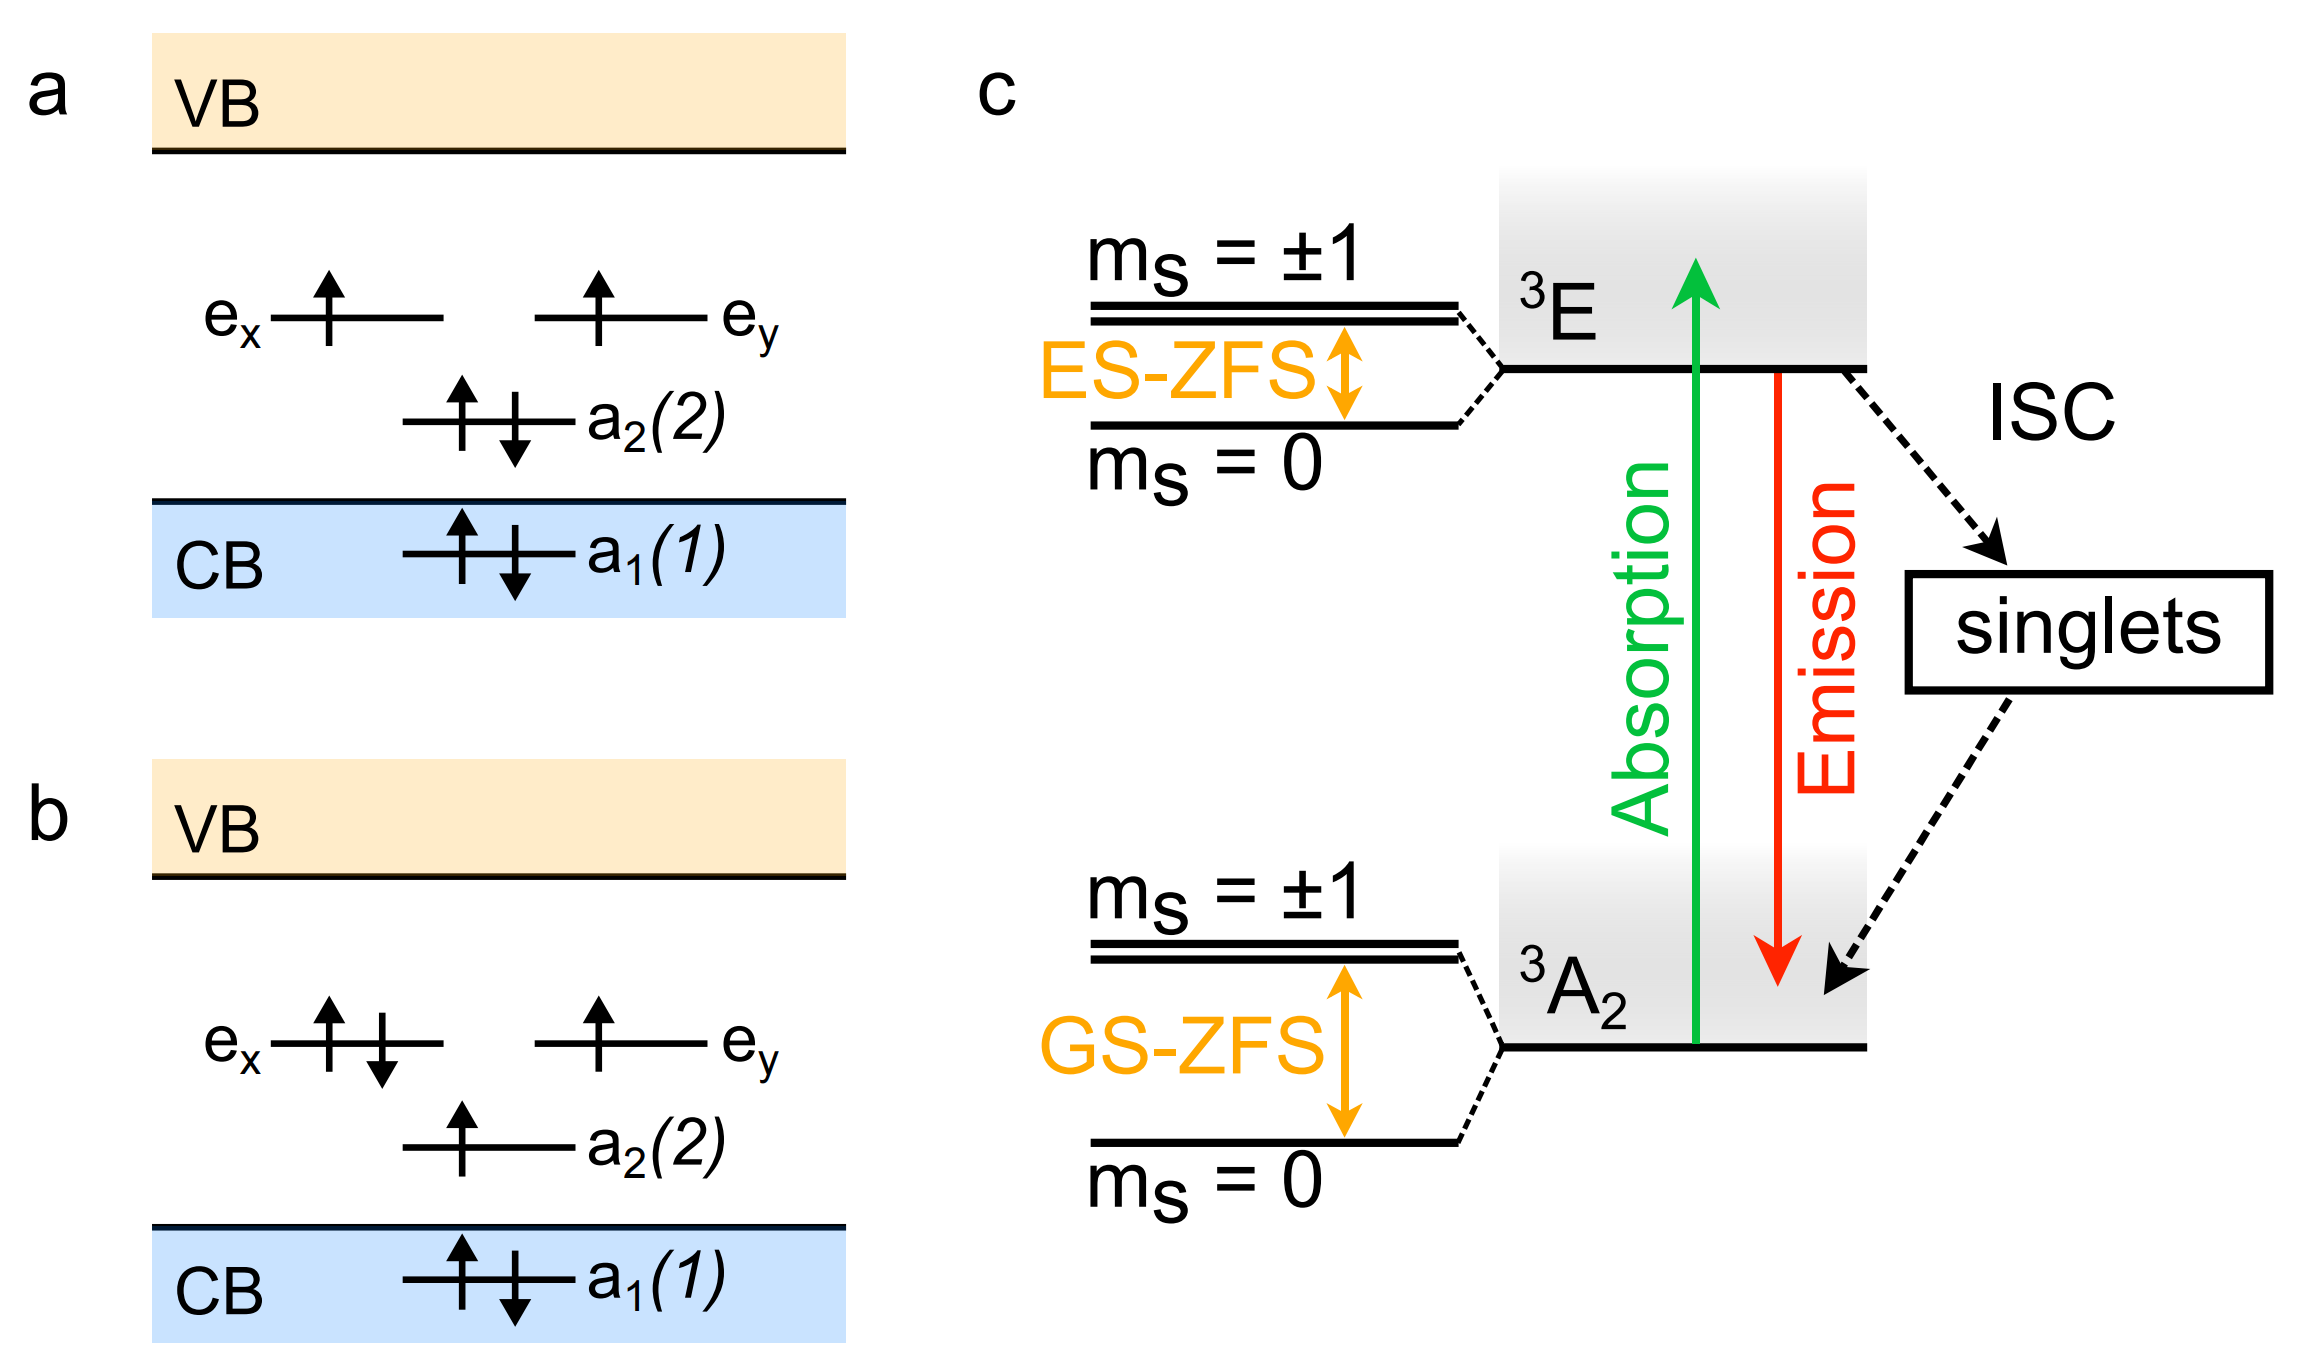
\includegraphics[width=1.0\textwidth]{figures/Chapter 1/Electronic Structure.png}
  \caption[NV$^-$的电子能级结构示意图]{NV$^-$的电子能级结构示意图,展示了带隙中间的缺陷能级:(a)$^3A_2$基态;(b)$^3E$激发态;(c)自旋三重态和ZPL跃迁过程,以及在自旋单态下的声子边带的ISC作用\cite{staudacher2015nuclear}。}
  \label{fig: Electronic Structure}
\end{figure}

需要注意的一点是,图 \ref{fig: Electronic Structure}中所展示的NV Center的电子能级结构仅仅是一个简单的示意图,更加详细的细节,比如自旋单态ISC过程的能级结构、电子和氮核自旋之间超精细相互作用(hyperfine interaction)在这里并没有详细的给出,这些内容会在后续的章节中有所涉及。

因为金刚石中电子的自旋-翻转作用需要通过金刚石晶体中的声子的释放来进行能量交换,所以NV自旋态之间的弛豫时间$T_1$与声子态密度有关。由于金刚石的德拜温度(Debye temperature)较高,所以声子态密度在环境室温的情况下较小,因此NV Center有着较低的电子-声子耦合性,从而有着较长的$T_1$弛豫时间\cite{koizumi2008physics}。较长的$T_1$时间与金刚石中较弱的自旋-轨道作用密切相关,其使得NV自旋态之间产生微小的混合状态,这些自旋态又与电子-声子相互作用发生耦合,从而使得NV自旋态发生弛豫。另外,因为金刚石较宽的带隙,所以NV Center存在于带隙中的缺陷能级受到外界环境的干扰较小,因此有着较高的稳定性。金刚石的这些独特的性质使得其在室温条件下,对于缺陷能级的跃迁效应不会有额外的影响,让NV Center的量子效应在室温情况下仍然可以被观测到并可以被用于量子信息、量子精密测量等领域,这一点相比于其他的量子体系,比如超导量子比特(superconducting qubit)、离子阱(trapped ions)等体系,有着非常大的优势\cite{hu2023progress, acosta2013nitrogen}。

\subsubsection{NV$^0$的电子能级结构}
对于NV$^0$而言,其电子能级结构和NV$^-$有所不同,如图 \ref{fig: NV0 Electronic Structure}所示。相对于有两个额外的未成对电子组成电子自旋量子数$S=1$的NV$^-$,NV$^0$的外部仅有一个额外的未成对电子,在光学激发的情况下,NV$^0$的能级结构可能是自旋量子数为$S=\frac{1}{2}$的自旋二重态(spin doublet)或$S=\frac{3}{2}$的自旋四重态(spin quadruplet state)。由于电子顺磁共振(electron paramagnetic resonance, EPR)实验过程中的干扰,Jahn-Teller畸变的效应对于NV$^0$的自旋二重态的影响较大,因此中性电荷态的NV Center并不适合各种各样基于电子自旋相关的测量,所以绝大部分的研究都是基于NV$^-$的电子自旋态进行的\cite{gali2009theoryoftheneutral}。然而,NV$^0$的电子能级结构对于NV$^-$的电子能级结构的理解和研究仍然有着重要的意义,比如在NV$^-$的电子自旋态和氮核自旋态之间的超精细相互作用的研究中,NV$^0$的电子能级结构可以作为NV$^-$的电子能级结构的参考,从而可以更好地理解NV$^-$的电子能级结构\cite{gali2009theoryoftheneutral}。

\begin{figure}
  \centering
  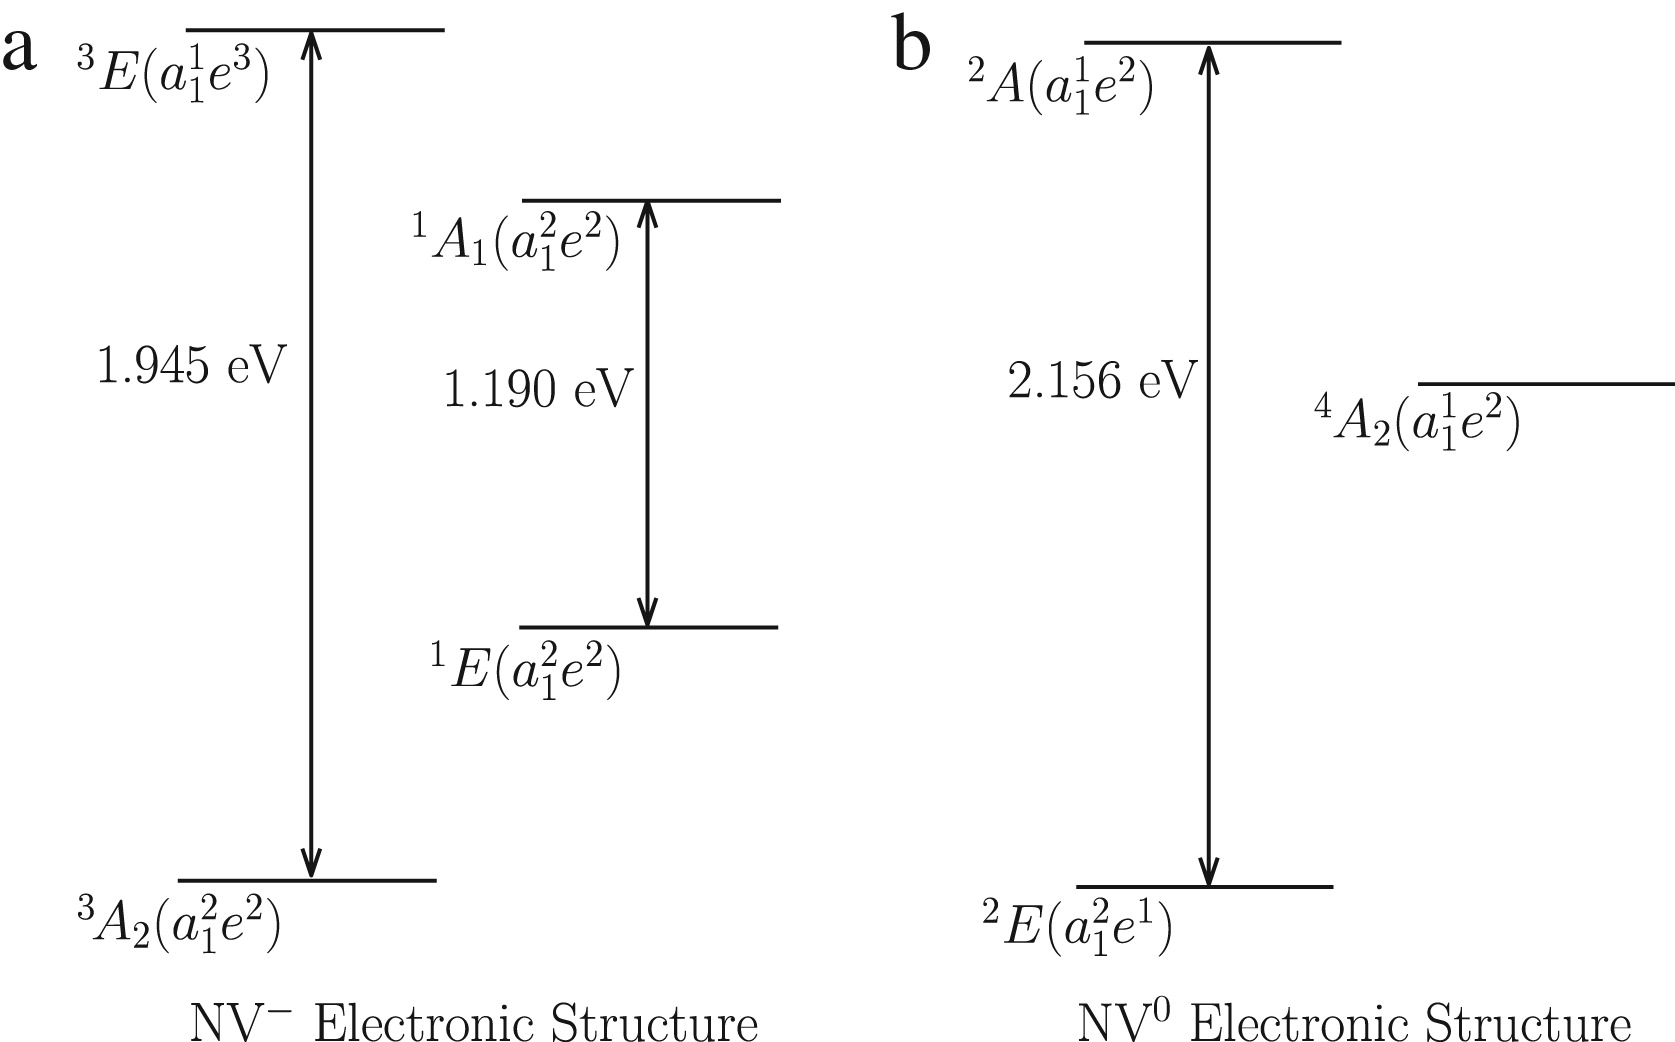
\includegraphics[width=0.9\textwidth]{figures/Chapter 1/NV0 Electronic Structure.jpg}
  \caption[NV$^-$和NV$^0$的电子能级结构对比]{NV$^-$和NV$^0$的电子能级结构对比,a图和b图分别展示了NV$^-$和NV$^0$的基态、激发态、声子边带的能级结构。图中分别NV$^-$和NV$^0$的ZPL能量,分别为1.945 eV(637 nm)和2.156 ev(575 nm),其中对于NV$^-$而言,声子边带的基态和激发态之间的能量差为1.190 eV(1041 nm)\cite{doherty2013nitrogen}。}
  \label{fig: NV0 Electronic Structure}
\end{figure}

本文的工作和研究主要依靠NV$^-$的基态和激发态自旋三重态,以及NV$^0$的基态和激发态的自旋双重太,包括他们的能级跃迁过程,因为这些决定了我们可以观测到的荧光效应,并由此来表征NV Center的各种性质。除此之外,这些荧光效应是光子激发电离过程的基础,因为它们在双光子激发自旋三重态和双重态的过程中,使得金刚石导带和价带的电子产生交换关联的效应,从而让荧光现象有着可观测的规律来让人们进行研究和应用\cite{aslam2013photo}。需要提到的一点是,对于ISC过程而言,也就是NV$^0$的自旋四重态和NV$^-$的自旋单态,在本文所研究的电荷态动力学这一关注点之下是可以忽略的,因为在目前的科学研究之中,这些状态时不参与NV Center的光致发光和光子激发电离的过程的。

\section{各节一级标题}
我是内容

\subsection{各节二级标题}
你是内容

\subsubsection{各节三级标题}
他是内容

\paragraph{四级标题}
内容内容

\subparagraph{五级标题}
内容内容

\section{字体样式}
宋体\quad \textbf{粗体}\quad \textit{斜体}\quad \textbf{\textit{粗斜体}}。

{\heiti 黑体\quad \textbf{粗体}\quad \textit{斜体}\quad \textbf{\textit{粗斜体}}}。

{\fangsong 仿宋\quad \textbf{粗体}\quad \textit{斜体}\quad \textbf{\textit{粗斜体}}}。

{\kaishu 楷书\quad \textbf{粗体}\quad \textit{斜体}\quad \textbf{\textit{粗斜体}}}。

Serif\quad \textit{Italic}\quad \textbf{Bold}\quad \textbf{\textit{BoldItalic}}

{\sffamily Sans\quad \textit{Italic}\quad \textbf{Bold}\quad \textbf{\textit{BoldItalic}}}

{\ttfamily Mono\quad \textit{Italic}\quad \textbf{Bold}\quad \textbf{\textit{BoldItalic}}}

\end{document}
\documentclass[type = bachelor]{whu-thesis}
\usepackage{textcomp,mathcomp}
\usepackage{siunitx}
\usepackage{chemfig}
\usepackage{graphicx}

\whusetup
  {
    info               =
      {
        title          = {金刚石氮-空位色心的\\电荷态调控和性质表征},
        title*         = {Modulation of Charge States and Characterization of Properties\\ in Nitrogen-Vacancy Centers of Diamond},
        student-number = {2020302192129},
        school         = {弘毅学堂},
        author         = {邹迪玮},
        author*        = {Diwei Zou},
        subject        = {学科},
        major          = {微电子科学与工程},
        advisor        = {周利 , 副教授;孙启超 , 研究员},
        direction      = {研究方向},
        date           = {2024/5},
        keywords       = {关键词 1 , 关键词 2 , 关键词 3 , 关键词 4 , 一个非常非常,非常非常长——的关键词 5},
        keywords*      = {key word 1 , key word 2 , key word 3 , key word 4 , {and a very very, very very long key word---the key word 5}},
      },
    style              =
      {
        graphics-path  = {{figures/}{data/}},
        list-of-figures,
        list-of-tables,
      },
    element            =
      {
        innovation     = {pages/innovation},
        abstract       = {pages/abstract},
        abstract*      = {pages/enabstract},
        bibliography   = {ref/refs_2}
      }
  }
\begin{document}


% Chapter 2

\chapter{NV Center电荷态动力学的理论原理}

\section{NV Center的电荷态}
因为NV Center电荷态的一些最基本的性质和特征已经在第一章中有所分析,所以本章主要聚焦于NV Center电荷态动力学的理论原理,也就是本文后续实验中所主要研究的对象和内容。本文主要研究的对象是NV Center的负电状态NV$^-$和中性状态NV$^0$,而NV Center的正电状态NV$^+$由于其电子结构的特殊性,其电荷态动力学的研究相对较少,所以本文不做过多的讨论\cite{schreyvogel2016active}。

\subsection{NV Center电荷态的荧光光谱}

在第一章的图 1.7中,我们可以看到NV Center的不同电荷态的荧光发射光谱的特征。在NV Center的荧光光谱中,我们可以看到NV$^-$和NV$^0$的荧光峰分别位于$637$ nm和$575$ nm处,。在实验中,我们可以通过测量NV Center的荧光光谱来判断其电荷态,从而可以对NV Center的电荷态进行观测和表征。

\begin{figure}
  \centering
  \includegraphics[width=1.0\textwidth]{figures/Chapter 2/Excitation Process.png}
  \caption[ZPL激发过程中电子的能级结构]{ZPL激发过程中电子的能级结构,上下两个区域中填充的浅绿色和粉红色部分分别表示价带最高点(valance band maximum, VBM)和导带最低点(conductive band minimum, CBM)。黑色横线表示价带和导带中不同能级,而中间透明区域中紫色横线表示带隙缺陷能级。分成左右两列绘制了$\alpha$-自旋向上和$\beta$-自旋向下的轨道。蓝色实箭头表示电子占据情况,而空心蓝色箭头表示在$^3A_2$ GS和$^3E$ ES中激发或退激发过程后的电子占据情况。}
  \label{fig: Excitation Process}
\end{figure}

在NV$^-$和NV$^0$的两个光谱曲线中,可以看到声子边带(phonon sidebands, PSB)的作用强度都比ZPL的强度更高,这个过程可以用利用基于Born-Oppenheimer近似和Franck-Condon原理的Huang-Rhys模型来进行简单地描述,即在分子或晶体中,当电子从其基态激发到一个激发态时,会导致与电子激发相关的振动模式被激发。这些振动模式的能级通常称为 "振动激发" 或 "振动副态",而Huang-Rhys 模型用来描述这些振动激发的分布和对电子激发的影响,如图 \ref{fig: Franck-Condon} a\cite{zou2023influence}。在这个模型之中,Huang-Rhys因子$S$决定了晶体结构在基态和激发态之间平衡态位置的差异,这个差异体现了吸收和发射光谱之间的斯托克斯能量位移$E_{Stokes}$。斯托克斯能量唯一和Huang-Rhys因子之间的关系取决于温度,在极低温的时候,光谱曲线中ZPL会有一个较为明显和尖锐的峰值,如图 \ref{fig: Franck-Condon} b所示;而基态和激发态能级之间的能量差异导致的光谱线会随着温度的升高而展宽,一个比较粗略的计算式如下: 
\begin{equation}
  S = (\frac{E_{Stokes}}{2\hbar \omega}+\frac{1}{4})±\frac{1}{4}
\end{equation}
其中$\hbar \omega$代表着缺陷周围晶体的平均声子能量\cite{de2015resolving}。对于NV Center而言,其Huang-Rhys因子在温度较低的情况下的数值一般为2.5 - 5,这表明了激发态相对于基态的结构在空间上有着比较大的偏移,这是两种电荷状态在光谱中决定声子边带形状的关键因素。在ZPL激发的过程中,电子在缺陷能级的占据情况可以通过基于第一性原理的密度泛函理论来计算出来,在仿真的过程中同样遵循Born-Oppenheimer近似和Franck-Condon原理,如图 \ref{fig: Excitation Process}所示,电子在跃迁的过程中保持自旋守恒的状态,仿真是基于Vienna Ab-initio Simulation Package(VASP)软件和杂化泛函Heyd-Scuseria-Ernzerhof (HSE06)算法得到的结果\cite{zou2023influence}。


\begin{figure}
  \centering
  \includegraphics[width=1.0\textwidth]{figures/Chapter 2/Franck-Condon.png}
  \caption[基于Born-Oppenheimer近似和Franck-Condon原理的Huang-Rhys模型示意图]{基于Born-Oppenheimer近似和Franck-Condon原理的Huang-Rhys模型示意图,展示了体系能量(E)和晶体结构坐标(q)的关系。纵轴上的E$_{ground}$和E$_{excited}$分别代表着基态和激发态准抛物线近似能量面的最低能量值,横轴上的q$_{ground}$和q$_{excited}$代表着基态和激发态晶体结构的平衡位置。ZPE为零点能(zero-point energy),最小能量比准抛物线的最低点稍高。}
  \label{fig: Franck-Condon}
\end{figure}

对于本文的工作而言,最重要的是要提高NV$^-$相对于NV$^0$的荧光计数率的比值,所有的计数率都是由基于雪崩光电二极管(Avalanche Photo Diodes, APDs)原理所开发的单光子探测器(Single Photon Detector, SPD)。根据第一章中的图 1.7中所展示的NV$^-$和NV$^0$的光谱曲线的不同,在实验中会在APDs前加入一个650 nm的长通滤光片,这样在收集到的光子中,主要来源则是NV$^-$的荧光发射光子,而NV$^0$的荧光发射的大部分光子则会被滤光片所阻挡。这样,我们就可以通过测量APDs的计数率来判断NV Center的电荷态,从而可以对NV Center的电荷态进行观测和表征。

单光子激发NV Center从基态跃迁到激发态然后退激发的荧光过程中,激发态有一定的寿命,这个寿命和其周围金刚石晶体的声子的活跃性有关,在寿命时间之后,激发态会自发地退激发到基态,这个过程会伴随着荧光光子的发射,发射出的光子波长和其能量有关,而能量则取决于跃迁能量和声子在激发过程中的振动能量。由于这是一个单光子过程,所以在较低的激发激光的功率下,两种电荷态的荧光计数率和光强是成线性的关系,也就是激光功率决定了可以到达NV Center并参与激发过程的光子的数量\cite{aslam2013photo}。对于单个NV Center而言,其可以作为光子发射的结构,由于激发态有一定的寿命,所以发射的荧光强度随着激发光强的提高,会出现饱和的现象。在激发光强超过饱和光强$P_{Sat}$的时候,NV Center的荧光强度将不再明显地增加,拟合公式为:
\begin{equation}
  F \propto N_2 +AP = C \frac{P/P_{Sat}}{1+P/P_{Sat}}+AP
\end{equation} 
其中$F$为单光子探测器单位时间内的读数,$N_2$为激发态布居数,$P$为当前激光强度,$P_{Sat}$为饱和激光强度,$AP$为激光漏光进入单光子探测器的读数,其数值正比于激光强度,通常情况下拟合曲线如图 \ref{fig: Saturation Plot}所示,从图中可以看出其饱和激发光强是854.86 \unit{\uW},该光强下的NV Center荧光发光的计数率为70.21 kpcs/s。金刚石表面的吸收和散射会导致激光功率的损失,所以在制备样品的过程中,我们在金刚石表面设计了纳米立柱(nano pillar)结构,然后将氮离子注入其中,再退火形成位于nano pillar结构中NV Center,如图 \ref{fig: nano pillar}。

\begin{figure}
  \centering
  \includegraphics[width=1.0\textwidth]{figures/Chapter 2/Saturation Plot.png}
  \caption[单个NV Center光强饱和曲线]{单个NV Center光强饱和曲线,横轴是激发光强,纵轴是APDs计数率,图中展示了饱和激发光强的大小和该情况下NV Center荧光发光的计数率。}
  \label{fig: Saturation Plot}
\end{figure}

\begin{figure}
  \centering
  \includegraphics[width=1.0\textwidth]{figures/Chapter 2/nano pillar.png}
  \caption[金刚石表面nano pillar结构]{金刚石表面nano pillar结构}
  \label{fig: nano pillar}
\end{figure}

\subsection{NV Center电荷态之间的电离和复合过程}
对于NV Center的两种电荷态NV$^-$和NV$^0$,它们之间有相互转换的机制,即缺陷能级电子的电离和复合(ionization and recombination)的过程,如图 \ref{fig: Ionization and Recombination}所示。

图 \ref{fig: Ionization and Recombination}a和b展示了从NV$^-$到NV$^0$的电离过程。在这个过程中,第一个光子激发NV$^-$基态能级的电子到激发态,紧接着第二个光子激发同一个电子,使其从带隙中的缺陷能级激发到金刚石导带能级,这让NV Center成为仅有一个未成对电子的电中性NV$^0$状态。图 \ref{fig: Ionization and Recombination}c和d展示了从NV$^0$到NV$^-$的复合过程,一个电子从NV$^0$自旋双重态的基态跃迁到激发态,和金刚石价带中的一个激发的电子结合,从而使得缺陷能级中重新拥有两个未成对的电子,回到负电的NV$^-$状态。

\begin{figure}
  \centering
  \includegraphics[width=1.0\textwidth]{figures/Chapter 2/Ionization and Recombination.png}
  \caption[NV Center带隙中缺陷能级电子的电离和复合过程]{NV Center带隙中缺陷能级电子的电离和复合过程\cite{aslam2013photo}。}
  \label{fig: Ionization and Recombination}
\end{figure}

不论是电离还是复合的过程,光电子的动力学特征都极其依赖于激光的波长,如图 \ref{fig: Different Wavelength}。因此,当激发光路波长在637 nm的时候,NV Center中的NV$^-$的占比将会随着时间急剧下降,即被电离为NV$^0$;532 nm的激发光子会将NV Center的电荷态向着NV$^-$占比更高的方向进行初始化。而本文中最重要的一个调控方式就是利用594 nm波长的黄橙光来抑制中性的NV$^0$结合电子从而复合成负电中心的NV$^-$。在这个激发的条件下,NV$^-$基态处于$m_s = 0, ±1$的电子都会被激发到激发态。由于存在ISC过程,之前处于基态$m_s = ±1$的电子会落到自旋单态的能级,而之前处于基态$m_s=0$的电子则会回到激发态$m_s=0$能级。然后功率较高的637 nm激光快速脉冲使得这些处于激发态$m_s=0$能级的电子激发到金刚石晶体的导带,从而使得NV Center呈现NV$^0$的电中性状态,而此时处于自旋单态的电子回到基态$m_s=0$的能级,这样使得将NV$^-$的自旋分布情况转换成可以读出的电荷分布状态。最后利用较低功率的594 nm的激光对这些回到基态$m_s=0$的能级的自旋状态进行长时间的读出并记录,通过荧光效应来观测并推导出电荷态的分布,通过APDs计数率的变化可以明显的看到这一过程,在594 nm激光连续波(continuous wave, CW)的持续作用下,我们可以观测到NV$^-$(高计数率)和NV$^0$(低计数率)之间存在一个特定的比例关系\cite{waldherr2011dark}。在这里,我们之所以使用594 nm的橙光来进行读出,是因为这个波长的光子能量比532 nm的能量稍低,可以防止将NV$^0$的电子激发,使之和价带电子结合,从而回到NV$^-$的状态,这样就将NV$^0$的状态保护了起来,便于读出信息,而不会像532 nm的光子会将NV Center初始化到NV$^-$的$m_s=0$。ll

\begin{figure}
  \centering
  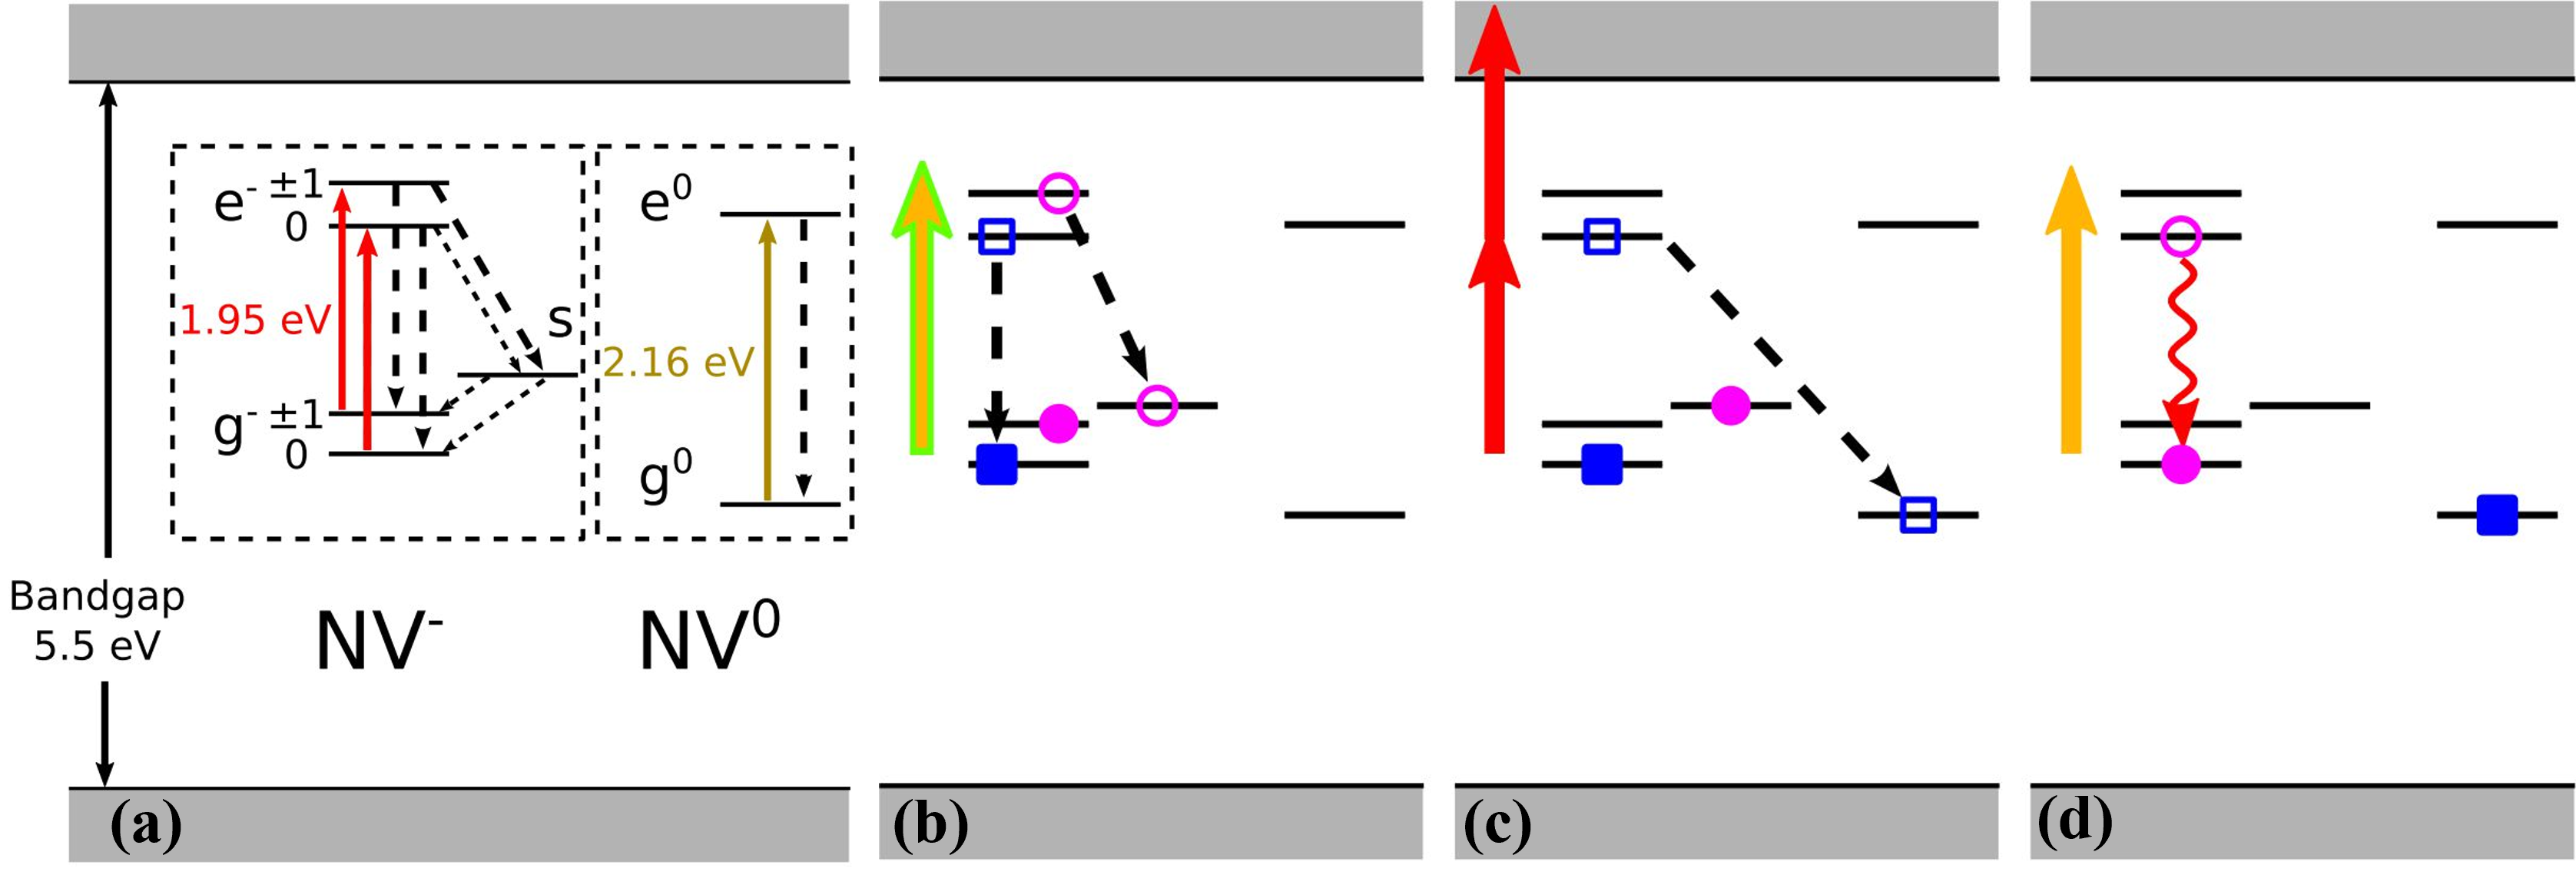
\includegraphics[width=1.0\textwidth]{figures/Chapter 2/Different Wavelength.png}
  \caption[NV$^-$和NV$^0$的电子能级结构和不同波长激光对于电子的调控]{NV$^-$和NV$^0$的电子能级结构和不同波长激光对于电子的调控,a、b、c分别是532 nm的绿光(或594 nm的黄橙光)、637 nm的红光、594 nm的黄橙光\cite{shields2015efficient}。}
  \label{fig: Different Wavelength}
\end{figure}

这些现象表明,NV Center的电荷态随着时间的变化并不是一个稳定的情况,而是有一个动态变化的状态,可以通过随着时间变化的相对电离和复合率来描述,这也是本文主要聚焦的问题。由于电离和复合的过程都可以用双光子过程来描述,因此在激光功率较低的时候,NV Center的荧光效应没有饱和前,电离和复合和激光光强有关,在后续的分析中需要考虑饱和光强这一限制因素。

除此之外,NV Center电荷态的电离和复合过程同样受到环境的影响,包括样品的晶体结构、掺杂等因素,以及环境温度、磁场、电场等实验环境因素,这些会在没有任何荧光效用的情况下影响NV Center的电荷态。比如,在制备样品的过程中,金刚石晶体中的一些缺陷结构会形成局域电子势阱(local electron traps),在NV$^-$转化为NV$^0$之后停止光学激发,电子将不会回落到NV Center缺陷能级附近,使得其变为暗态\cite{bluvstein2019identifying}。除此之外,一些施主掺杂元素在没有外界激发的激发的情况下,也会在一定程度上影响NV$^-$的布局数分布\cite{doi2016pure}。本人也曾利用基于第一性原理的密度泛函理论探究并证明了相比于实验中最为常见的氮元素施主掺杂的金刚石中的NV Center而言,磷元素施主掺杂的金刚石中的NV$^-$在保证其原有的量子比特的各种优异性质的同时,其NV Center的负电中心稳定性更强\cite{zou2023influence}。

\section{NV Center电荷态动力学的理论模型}
在这一部分,本文将基于B. J. Shields和L. Hacquebard等人提出的方案,对于NV Center电荷态动力学的理论模型进行构建和分析\cite{shields2015efficient, hacquebard2018charge}。NV Center的荧光发光特征可以通过在时间尺度记录APDs所收集到的单光子计数率来表征,当NV Center处于NV$^-$状态的时候,会有较高的计数率$\gamma_-$;当NV Center处于NV$^0$状态的时候,会有较低的计数率$\gamma_0$。$\gamma_-$和$\gamma_0$在本文后续都分别指代NV$^-$和NV$^0$的计数率,并用这两个可以直接探测到的参数在特定的读出时间(readout time)$t_r$区间下来构建收集到光子数结果的直方图。如果在一定的读出时间$t_r$之中,NV Center的电荷态没有发生改变,那这个可以用两个泊松概率分布函数(Poissonian Probability Distribution Functions, PPDF)来分别描述NV$^0$和NV$^0$态的布居数分布直方图:
\begin{equation}
  PPDF_0(n, \gamma_0 t_r) = \frac{(\gamma_0 t_r)^n exp(-\gamma_0 t_r)}{n!}
  \label{equ: PPDF_0}
\end{equation}
\begin{equation}
  PPDF_-(n, \gamma_- t_r) = \frac{(\gamma_- t_r)^n exp(-\gamma_- t_r)}{n!}
  \label{equ: PPDF_1}
\end{equation}
由于计数率的单位与时间相关,通常为kpcs/s(千光子每秒),而且荧光的光子在特定的读出时间中是随机的统计分布,也就是在自然情况下遵循泊松分布,即所以读取到特定电荷态计数率的均值为$\gamma_0 t_r$或$\gamma_- t_r$,作为泊松分布函数的变量,因此在一定的读出时间$t_r$之中,探测到的光子数量$n$的直方图可以计算:
\begin{equation}
P_{hist}(n)=P(NV^0)PPDF_0(n, \gamma_0 t_r)+P(NV^-)PPDF_-(n, \gamma_- t_r)
\end{equation}
其中$P(NV^0)$和$P(NV^-)$是在读出时间$t_r$的开始,NV Center处于特定电荷态的概率,两种状态的初始概率分别由单个泊松分布在总面积中占据的比例决定的。

然而,前文所讨论的NV Center缺陷电子能级结构中,未成对电子的电离和复合对应的电荷态的转换及其过程中的荧光效应的描述是一个简化模型,实际上电荷态在读出时间的尺度之内是极其不稳定的,可能会在这个时间段内发生数次电荷态的转换,这种电荷态转换可以用从NV$^0$到NV$^-$的复合率$g_{0-}$和从NV$^-$到NV$^0$的电离率$g_{-0}$这两个参数来描述。为了简单理解这样的电荷态动态转化的过程,可以用一些简单的例子来说明,如图 \ref{fig: Charge Conversion}a所示。在这个$t_r$的过程中,初始的电荷态为NV$^0$,持续时间为$\tau_1$,然后复合形成NV$^-$的概率为:
\begin{equation}
  p_1(\tau_1,g_{0-}) = g_{0-}\tau_1 \cdot e^{-g_{0-}\tau_1}
\end{equation}
这个式子为PPDF公式\ref{equ: PPDF_0}简单形式,其中$n=1$,$\gamma_0 = g_{0-}$,$t_r=\tau_1$。
同样的,对于序列的第二段和第三段而言,其概率为:
\begin{equation}
  p_2(t_1,g_{-0}) = g_{-0}t_1 \cdot e^{-g_{-0}t_1}
\end{equation}
\begin{equation}
  p_3(\tau_2,g_{0-}) = \tau_2 \cdot e^{-g_{0-}\tau_2}
\end{equation}
需要注意的是,我们假设在第三部分后,不会有电荷转换的情况产生,所以系数中不存在$g_{0-}$这一项。对于时间而言,有$\tau=\tau_1+\tau_2$和$t_r-\tau=t_1$,所以整体的概率为上述三个概率的乘积:
\begin{equation}
  \begin{aligned}
    P_a(\tau,t_r,g_{0-},g_{-0}) &= p_1 \cdot p_2 \cdot p_3 \\
    &= g_{0-}g_{-0}\tau_1\tau_2t_1 \cdot e^{(g_{-0}-g_{0-})\tau-g_{-0}t_r}
  \end{aligned}
\end{equation}
同样的,对于另外三种可能的情况,概率计算的结果如下:
\begin{equation}
  P_b(\tau,t_r,g_{0-},g_{-0}) = g_{-0}g_{0-}\tau_1\tau_2t_1 \cdot e^{(g_{0-}-g_{-0})\tau-g_{0-}t_r}
\end{equation}
\begin{equation}
  P_c(\tau,t_r,g_{0-},g_{-0}) = g_{0-}\tau_1t_1 \cdot e^{(g_{-0}-g_{0-})\tau-g_{-0}t_r}
\end{equation}
\begin{equation}
  P_c(\tau,t_r,g_{0-},g_{-0}) = g_{-0}\tau_1t_1 \cdot e^{(g_{0-}-g_{-0})\tau-g_{0-}t_r}
\end{equation}

\begin{figure}
  \centering
  \includegraphics[width=1.0\textwidth]{figures/Chapter 2/Charge Conversion.png}
  \caption[不同电荷初态时,NV Center电荷态的转换过程示意图]{不同电荷初态时,NV Center电荷态的转换过程示意图,观测的时间尺度为读出时间$t_r$, $\tau_i$为在$t_r$中和初始电荷态相同状态所持续的时间,$t_i$为在$t_r$中和初始电荷态不同状态所持续的时间。(a)初始电荷态为NV$^0$,且电荷态的转换次数为偶数;(b)初始电荷态为NV$^-$,且电荷态的转换次数为偶数;(c)初始电荷态为NV$^0$,且电荷态的转换次数为奇数;(d)初始电荷态为NV$^-$,且电荷态的转换次数为奇数。}
  \label{fig: Charge Conversion}
\end{figure}

在图 \ref{fig: Charge Conversion}中所展示的是在读出时间$t_r$中最基本的四种序列,分类依据是初始电荷态是NV$^-$或者NV$^0$以及电荷态转换的次数是奇数次或者偶数次。更一般的情况下,可以将这些情况进行组合,并且可能会有很多次的电荷态转换的现象产生,所以可以写出更为普适性的表达式,即对上面推导的式子分情况进行积分和求和:
\begin{equation}
  \begin{aligned}
    p(n|NV^0,even)=&\int_{0}^{t_r}d\tau e^{(g_{-0}-g_{0-})\tau-g_{-0}t_r} \sum_{i=1}^{\infty}(g_{0-}g_{-0})^i \prod_{j=1}^{i}\int_{0}^{\tau-\sum_{k=1}^{j-1}\tau_k}d\tau_j \\
    & \times \prod_{j=1}^{i-1}\int_{0}^{(t_r-\tau)-\sum_{k=1}^{j-1}t_k}dt_jPPDF(n, \gamma_0\tau+\gamma_-(t_r-\tau)) \\
    & + e^{-g_{0-}t_r}PPDF(n, \gamma_0t_r)
  \end{aligned}
\end{equation}
\begin{equation}
  \begin{aligned}
    p(n|NV^-,even)=&\int_{0}^{t_r}d\tau e^{(g_{0-}-g_{-0})\tau-g_{0-}t_r} \sum_{i=1}^{\infty}(g_{-0}g_{0-})^i \prod_{j=1}^{i}\int_{0}^{\tau-\sum_{k=1}^{j-1}\tau_k}d\tau_j \\
    & \times \prod_{j=1}^{i-1}\int_{0}^{(t_r-\tau)-\sum_{k=1}^{j-1}t_k}dt_jPPDF(n, \gamma_-\tau+\gamma_0(t_r-\tau)) \\
    & + e^{-g_{-0}t_r}PPDF(n, \gamma_-t_r)
  \end{aligned}
\end{equation}
\begin{equation}
  \begin{aligned}
    p(n|NV^0,odd)=&\int_{0}^{t_r}d\tau e^{(g_{-0}-g_{0-})\tau-g_{-0}t_r} \sum_{i=1}^{\infty}g_{0-}^ig_{-0}^{i-1} \prod_{j=1}^{i-1}\int_{0}^{\tau-\sum_{k=1}^{j-1}\tau_k}d\tau_j \\
    & \times \prod_{j=1}^{i-1}\int_{0}^{(t_r-\tau)-\sum_{k=1}^{j-1}t_k}dt_jPPDF(n, \gamma_0\tau+\gamma_-(t_r-\tau)) \\
    & + e^{-g_{0-}t_r}PPDF(n, \gamma_0t_r)
  \end{aligned}
\end{equation}
\begin{equation}
  \begin{aligned}
    p(n|NV^-,odd)=&\int_{0}^{t_r}d\tau e^{(g_{0-}-g_{-0})\tau-g_{0-}t_r} \sum_{i=1}^{\infty}g_{-0}^ig_{0-}^{i-1} \prod_{j=1}^{i-1}\int_{0}^{\tau-\sum_{k=1}^{j-1}\tau_k}d\tau_j \\
    & \times \prod_{j=1}^{i-1}\int_{0}^{(t_r-\tau)-\sum_{k=1}^{j-1}t_k}dt_jPPDF(n, \gamma_-\tau+\gamma_0(t_r-\tau)) \\
    & + e^{-g_{-0}t_r}PPDF(n, \gamma_-t_r)
  \end{aligned}
\end{equation}
这四个通用公式是由M. D. Lukin及其团队在2015年提出的,用以解释电荷态在一定的读出时间内转换的普适性概率模型 \ref{shields2015efficient}。由这个公式,我们可以得到在这个读出时间段内光子数$n$的直方图计算表达式:
\begin{equation}
  \begin{aligned}
    P(n)&=P(NV^0)[p(n|NV^0,even)+p(n|NV^0,odd)] \\
    &+P(NV^-)[p(n|NV^-,even)+p(n|NV^-,odd)] \\
    &=P(NV^0)p(n|NV^0)+P(NV^-)p(n|NV^-)
  \end{aligned}
\end{equation}
由这个式子可以得到,在这个模型中,只剩下初始态处于NV$^0$或NV$^-$的概率$P(NV^0)$和$P(NV^-)$需要来确定,由此我们需要进行连续波(continuous wave)和脉冲(pulsed)测量来分布确定所需要的数据,这里的连续波和脉冲测量指的是在读出时间内激光是否会间断。

\subsection{CW测量下初始电荷态分布和读出保真度}
一旦知道了电荷态转换率$g_{-0}$和$g_{0-}$,电荷态动力学分布就可以用下面两个微分系统方程来描述:
\begin{equation}
  \dot{\rho}_- = g_{0-}\rho_0-g_{-0}\rho_-
  \label{equ: differential equations_-}
\end{equation}
\begin{equation}
  \dot{\rho}_0 = -g_{0-}\rho_0+g_{-0}\rho_-
  \label{equ: differential equations_0}
\end{equation}
其中$\rho_-$是负电荷态总体概率分布,而$\rho_0$是中性电荷态总体分布的概率,即:
\begin{equation}
  P(NV^-) \equiv \rho_-
\end{equation}
\begin{equation}
  P(NV^-) \equiv 1-\rho_- = \rho_0
\end{equation}
然而,在恒定功率和波长的激光CW激发测量下,系统中的电荷态是近乎稳定,也就是$\dot{\rho}_0 = \dot{\rho}_- = 0$,因此由式\ref{equ: differential equations_-}和\ref{equ: differential equations_0}可以得到:
\begin{equation}
  \frac{g_{0-}}{g_{-0}}=\frac{\rho_-}{\rho_0}
\end{equation}
\begin{equation}
  P(NV^-)=\frac{g_{0-}}{g_{0-}+g_{-0}}
\end{equation}
通过这些计算,可以构建利用CW测量电荷态的模型和实验方案。

另外一个比较重要的特征是我们可以通过CW测量来得到读出保真度$\mathcal{F}_C$,也就是我们能够顺利读出并正确判断电荷态的可信度。其中一个关键点是设定一个合适的光子计数率阈值$n_{thresh}$来区分NV$^0$和NV$^-$的分布状态。因为NV$^0$状态时的计数率要远低于NV$^-$,所以在一定的读出时间$t_r$之中,如果计数率低于$n_{thresh}$,则计入NV$^0$的部分,反之则计入NV$^-$的部分。读出效率的公式可以由此计算:
\begin{equation}
  \mathcal{F}_c = \frac{1}{2}[\sum_{n=0}^{n_{thresh}}p(n|NV^0)+\sum_{n_{thresh}}^{n_{max}}p(n|NV^-)]
\end{equation}
我们需要最大化读出效率,所以需要对于读出594 nm橙光的功率$P$和读出时间$t_r$进行测试和优化,从而使得$\mathcal{F}_C$达到尽可能大的数值,这对于基于单次读出激光来收集统计光子数的单次读出(single shot readout)技术而言非常重要。

除此之外,区分NV$^0$和NV$^-$的阈值$n_{thresh}$的设定同样十分重要。如图 \ref{fig: n_thresh}所示,左图(a)为实验中利用APDs测得的原始数据,展示了在读出时间$t_r$中不同时刻计数率的变化曲线,我们可以很明显可以看到,在其中计数率高的为NV$^-$,计数率低的为NV$^0$。而右图(b)则是将(a)图中的计数率转化为其概率密度分布的直方图,可以看到由明显的两个峰值,然后用两个泊松概率分布函数进行拟合,从而得到了两种电荷态的曲线,左边整体计数率低的峰的拟合曲线表示的是NV$^0$,右边整体计数率高的峰的拟合曲线表示的是NV$^-$,这两条曲线有一个交点,通常将这个交点设置为$n_{thresh}$来区分两种不同的电荷态,并用于计算读出保真度$\mathcal{F}_C$。

\begin{figure}
  \centering
  \includegraphics[width=1.0\textwidth]{figures/Chapter 2/n_thresh.png}
  \caption[计数率的统计和$n_{thresh}$的确定]{计数率的统计和$n_{thresh}$的确定,(a)图中展示了APDs计数率随着时间的变化趋势,(b)中的柱状图展示了讲计数率转化为概率密度分布的曲线\cite{aslam2013photo}。}
  \label{fig: n_thresh}
\end{figure}

\subsection{脉冲测量中初始化电荷态和初始化保真度$\mathcal{F}_I$}
当进行脉冲序列测量的时候,电荷态将不会保持一个稳定的状态,而是会随着初始化脉冲和读出脉冲的序列而发生变化。为了初始化电荷态,即将尽可能多的NV$^0$转化到NV$^-$的$m_s=0$态,在594 nm的橙光读出后,会紧跟着一束持续3000 ns的高功率532 nm的绿光脉冲来对NV Center进行初始化。这种方法的原理是基于不同波长的激光会对NV Center的电荷和复合产生比较大的影响。在532 nm的绿光脉冲的作用下,NV$^0$的电子会被激发到更高的能级,从而能和价带中或者电子势阱中的额外电子结合,使得NV Center回到NV$^-$的状态,而NV$^-$在基态三重态$m_s=±1$的电子则会被激发到NV$^-$的激发态,然后通过ISC过程回到NV$^-$的$m_s=0$基态,这样就使得NV Center被初始化。

脉冲测量的主要作用就是确定初始化保真度$\mathcal{F}_I$,而在施加绿光脉冲的过程中,NV$^-$的电离作用主要取决于绿光的功率,也就是说功率过高的绿光会将NV$^-$再次电离,这样就会降低电离的保真度,所以需要对于绿光的功率进行优化,使得初始化保真度$\mathcal{F}_I$达到最大值。$\mathcal{F}_I$可以通过随着时间变化的计数率直方图来计算,通过拟合初始的光子数来得到:
\begin{equation}
  P(n)_{ini}=(1-\mathcal{F}_I)p(n|NV^0)+\mathcal{F}_Ip(n|NV^-)
\end{equation}
其中$p(n|NV^0)$和$p(n|NV^-)$分别是NV$^0$和NV$^-$的概率分布,而$\mathcal{F}_I$则是初始化保真度,即初始化NV$^0$为NV$^-$的概率。在这个模型中,我们假设了在初始化脉冲之后,NV Center的电荷态不会发生改变,即在读出脉冲之前,NV Center的电荷态不会发生改变,这个假设在实验中是成立的,因为初始化脉冲的时间尺度远小于读出脉冲的时间尺度,所以在读出脉冲之前,NV Center的电荷态不会发生改变。

对于初始化保真度的优化同样十分重要,因为初始化脉冲在大部分涉及到NV Center的实验中,通常被用于在测量序列之前让尽可能多的NV Center转化为方便调控和读出的NV$^-$,并且提高NV Center用于量子信息领域时候较为重要的自旋相干时间这一参数\cite{robledo2011spin}。

\end{document}
\documentclass[type = bachelor]{whu-thesis}
\usepackage{textcomp,mathcomp}
\usepackage{siunitx}
\usepackage{chemfig}
\usepackage{graphicx}

\whusetup
  {
    info               =
      {
        title          = {金刚石氮-空位色心的\\电荷态调控和性质表征},
        title*         = {Modulation of Charge States and Characterization of Properties\\ in Nitrogen-Vacancy Centers of Diamond},
        student-number = {2020302192129},
        school         = {弘毅学堂},
        author         = {邹迪玮},
        author*        = {Diwei Zou},
        subject        = {学科},
        major          = {微电子科学与工程},
        advisor        = {周利 , 副教授;孙启超 , 研究员},
        direction      = {研究方向},
        date           = {2024/5},
        keywords       = {关键词 1 , 关键词 2 , 关键词 3 , 关键词 4 , 一个非常非常,非常非常长——的关键词 5},
        keywords*      = {key word 1 , key word 2 , key word 3 , key word 4 , {and a very very, very very long key word---the key word 5}},
      },
    style              =
      {
        graphics-path  = {{figures/}{data/}},
        list-of-figures,
        list-of-tables,
      },
    element            =
      {
        innovation     = {pages/innovation},
        abstract       = {pages/abstract},
        abstract*      = {pages/enabstract},
        bibliography   = {ref/refs_all}
      }
  }
\begin{document}


% Chapter 3

\chapter{NV Center电荷态动力学的理论原理}

\section{NV Center的电荷态}
因为NV Center电荷态的一些最基本的性质和特征已经在第一章中有所分析,所以本章主要聚焦于NV Center电荷态动力学的理论原理,也就是本文后续实验中所主要研究的对象和内容。本文主要研究的对象是NV Center的负电状态NV$^-$和中性状态NV$^0$,而NV Center的正电状态NV$^+$由于其电子结构的特殊性,其电荷态动力学的研究相对较少,所以本文不做过多的讨论\cite{Schreyvogel2016}。

\subsection{NV Center电荷态的荧光光谱}

在第一章的图 1.7中,我们可以看到NV Center的不同电荷态的荧光发射光谱的特征。在NV Center的荧光光谱中,我们可以看到NV$^-$和NV$^0$的荧光峰分别位于$637$ nm和$575$ nm处,。在实验中,我们可以通过测量NV Center的荧光光谱来判断其电荷态,从而可以对NV Center的电荷态进行观测和表征。

\begin{figure}
  \centering
  \includegraphics[width=1.0\textwidth]{figures/Chapter 3/Excitation Process.png}
  \caption[ZPL激发过程中电子的能级结构]{ZPL激发过程中电子的能级结构,上下两个区域中填充的浅绿色和粉红色部分分别表示价带最高点(valance band maximum, VBM)和导带最低点(conductive band minimum, CBM)。黑色横线表示价带和导带中不同能级,而中间透明区域中紫色横线表示带隙缺陷能级。分成左右两列绘制了$\alpha$-自旋向上和$\beta$-自旋向下的轨道。蓝色实箭头表示电子占据情况,而空心蓝色箭头表示在$^3A_2$ GS和$^3E$ ES中激发或退激发过程后的电子占据情况。}
  \label{fig: Excitation Process}
\end{figure}

在NV$^-$和NV$^0$的两个光谱曲线中,可以看到声子边带(phonon sidebands, PSB)的作用强度都比ZPL的强度更高,这个过程可以用利用基于Born-Oppenheimer近似和Franck-Condon原理的Huang-Rhys模型来进行简单地描述,即在分子或晶体中,当电子从其基态激发到一个激发态时,会导致与电子激发相关的振动模式被激发。这些振动模式的能级通常称为 "振动激发" 或 "振动副态",而Huang-Rhys 模型用来描述这些振动激发的分布和对电子激发的影响,如图 \ref{fig: Franck-Condon} a\cite{Zou2024}。在这个模型之中,Huang-Rhys因子$S$决定了晶体结构在基态和激发态之间平衡态位置的差异,这个差异体现了吸收和发射光谱之间的斯托克斯能量位移$E_{Stokes}$。斯托克斯能量唯一和Huang-Rhys因子之间的关系取决于温度,在极低温的时候,光谱曲线中ZPL会有一个较为明显和尖锐的峰值,如图 \ref{fig: Franck-Condon} b所示;而基态和激发态能级之间的能量差异导致的光谱线会随着温度的升高而展宽,一个比较粗略的计算式如下: 
\begin{equation}
  S = (\frac{E_{Stokes}}{2\hbar \omega}+\frac{1}{4})±\frac{1}{4}
\end{equation}
其中$\hbar \omega$代表着缺陷周围晶体的平均声子能量\cite{de2015resolving}。对于NV Center而言,其Huang-Rhys因子在温度较低的情况下的数值一般为2.5 - 5,这表明了激发态相对于基态的结构在空间上有着比较大的偏移,这是两种电荷状态在光谱中决定声子边带形状的关键因素。在ZPL激发的过程中,电子在缺陷能级的占据情况可以通过基于第一性原理的密度泛函理论来计算出来,在仿真的过程中同样遵循Born-Oppenheimer近似和Franck-Condon原理,如图 \ref{fig: Excitation Process}所示,电子在跃迁的过程中保持自旋守恒的状态,仿真是基于Vienna Ab-initio Simulation Package(VASP)软件和杂化泛函Heyd-Scuseria-Ernzerhof (HSE06)算法得到的结果\cite{Zou2024}。


\begin{figure}
  \centering
  \includegraphics[width=1.0\textwidth]{figures/Chapter 3/Franck-Condon.png}
  \caption[基于Born-Oppenheimer近似和Franck-Condon原理的Huang-Rhys模型示意图]{基于Born-Oppenheimer近似和Franck-Condon原理的Huang-Rhys模型示意图,展示了体系能量(E)和晶体结构坐标(q)的关系。纵轴上的E$_{ground}$和E$_{excited}$分别代表着基态和激发态准抛物线近似能量面的最低能量值,横轴上的q$_{ground}$和q$_{excited}$代表着基态和激发态晶体结构的平衡位置。ZPE为零点能(zero-point energy),最小能量比准抛物线的最低点稍高。}
  \label{fig: Franck-Condon}
\end{figure}

对于本文的工作而言,最重要的是要提高NV$^-$相对于NV$^0$的荧光计数率的比值,所有的计数率都是由基于雪崩光电二极管(Avalanche Photo Diodes, APDs)原理所开发的单光子探测器(Single Photon Detector, SPD)。根据第一章中的图 1.7中所展示的NV$^-$和NV$^0$的光谱曲线的不同,在实验中会在APDs前加入一个650 nm的长通滤光片,这样在收集到的光子中,主要来源则是NV$^-$的荧光发射光子,而NV$^0$的荧光发射的大部分光子则会被滤光片所阻挡。这样,我们就可以通过测量APDs的计数率来判断NV Center的电荷态,从而可以对NV Center的电荷态进行观测和表征。

单光子激发NV Center从基态跃迁到激发态然后退激发的荧光过程中,激发态有一定的寿命,这个寿命和其周围金刚石晶体的声子的活跃性有关,在寿命时间之后,激发态会自发地退激发到基态,这个过程会伴随着荧光光子的发射,发射出的光子波长和其能量有关,而能量则取决于跃迁能量和声子在激发过程中的振动能量。由于这是一个单光子过程,所以在较低的激发激光的功率下,两种电荷态的荧光计数率和光强是成线性的关系,也就是激光功率决定了可以到达NV Center并参与激发过程的光子的数量\cite{Aslam2013}。对于单个NV Center而言,其可以作为光子发射的结构,由于激发态有一定的寿命,所以发射的荧光强度随着激发光强的提高,会出现饱和的现象。在激发光强超过饱和光强$P_{Sat}$的时候,NV Center的荧光强度将不再明显地增加,拟合公式为:
\begin{equation}
  F \propto N_2 +AP = C \frac{P/P_{Sat}}{1+P/P_{Sat}}+AP
\end{equation} 
其中$F$为单光子探测器单位时间内的读数,$N_2$为激发态布居数,$P$为当前激光强度,$P_{Sat}$为饱和激光强度,$AP$为激光漏光进入单光子探测器的读数,其数值正比于激光强度,通常情况下拟合曲线如图 \ref{fig: Saturation Plot}所示,从图中可以看出其饱和激发光强是854.86 \unit{\uW},该光强下的NV Center荧光发光的计数率为70.21 kpcs/s。金刚石表面的吸收和散射会导致激光功率的损失,所以在制备样品的过程中,可以在金刚石表面设计了纳米立柱(nano pillar)结构,然后将氮离子注入其中,再退火形成位于nano pillar结构中NV Center,如图 \ref{fig: nano pillar}。不过受制于工艺的限制,我们制备的纳米立柱结构的单点NV Center发光并不稳定,所以本文实验所采用的样品仍然是以Element Six公司生产的金刚石样片表面注入生成的单点NV Center形成的点阵,并没有设计特殊结构。

\begin{figure}
  \centering
  \includegraphics[width=1.0\textwidth]{figures/Chapter 3/Saturation Plot.png}
  \caption[单个NV Center光强饱和曲线]{单个NV Center光强饱和曲线,横轴是激发光强,纵轴是APDs计数率,图中展示了饱和激发光强的大小和该情况下NV Center荧光发光的计数率。}
  \label{fig: Saturation Plot}
\end{figure}

\begin{figure}
  \centering
  \includegraphics[width=1.0\textwidth]{figures/Chapter 3/nano pillar.png}
  \caption[金刚石表面nano pillar结构]{金刚石表面nano pillar结构}
  \label{fig: nano pillar}
\end{figure}

\subsection{NV Center电荷态之间的电离和复合过程}
对于NV Center的两种电荷态NV$^-$和NV$^0$,它们之间有相互转换的机制,即缺陷能级电子的电离和复合(ionization and recombination)的过程,如图 \ref{fig: Ionization and Recombination}所示。

图 \ref{fig: Ionization and Recombination}a和b展示了从NV$^-$到NV$^0$的电离过程。在这个过程中,第一个光子激发NV$^-$基态能级的电子到激发态,紧接着第二个光子激发同一个电子,使其从带隙中的缺陷能级激发到金刚石导带能级,这让NV Center成为仅有一个未成对电子的电中性NV$^0$状态。图 \ref{fig: Ionization and Recombination}c和d展示了从NV$^0$到NV$^-$的复合过程,一个电子从NV$^0$自旋双重态的基态跃迁到激发态,和金刚石价带中的一个激发的电子结合,从而使得缺陷能级中重新拥有两个未成对的电子,回到负电的NV$^-$状态。

\begin{figure}
  \centering
  \includegraphics[width=1.0\textwidth]{figures/Chapter 3/Ionization and Recombination.png}
  \caption[NV Center带隙中缺陷能级电子的电离和复合过程]{NV Center带隙中缺陷能级电子的电离和复合过程\cite{Aslam2013}。}
  \label{fig: Ionization and Recombination}
\end{figure}

不论是电离还是复合的过程,光电子的动力学特征都极其依赖于激光的波长,如图 \ref{fig: Different Wavelength}。因此,当激发光路波长在637 nm的时候,NV Center中的NV$^-$的占比将会随着时间急剧下降,即被电离为NV$^0$;532 nm的激发光子会将NV Center的电荷态向着NV$^-$占比更高的方向进行初始化。而本文中最重要的一个调控方式就是利用594 nm波长的黄橙光来抑制中性的NV$^0$结合电子从而复合成负电中心的NV$^-$。在这个激发的条件下,NV$^-$基态处于$m_s = 0, ±1$的电子都会被激发到激发态。由于存在ISC过程,之前处于基态$m_s = ±1$的电子会落到自旋单态的能级,而之前处于基态$m_s=0$的电子则会回到激发态$m_s=0$能级。然后功率较高的637 nm激光快速脉冲使得这些处于激发态$m_s=0$能级的电子激发到金刚石晶体的导带,从而使得NV Center呈现NV$^0$的电中性状态,而此时处于自旋单态的电子回到基态$m_s=0$的能级,这样使得将NV$^-$的自旋分布情况转换成可以读出的电荷分布状态。最后利用较低功率的594 nm的激光对这些回到基态$m_s=0$的能级的自旋状态进行长时间的读出并记录,通过荧光效应来观测并推导出电荷态的分布,通过APDs计数率的变化可以明显的看到这一过程,在594 nm激光连续波(continuous wave, CW)的持续作用下,我们可以观测到NV$^-$(高计数率)和NV$^0$(低计数率)之间存在一个特定的比例关系\cite{Waldherr2011}。在这里,我们之所以使用594 nm的橙光来进行读出,是因为这个波长的光子能量比532 nm的能量稍低,可以防止将NV$^0$的电子激发,使之和价带电子结合,从而回到NV$^-$的状态,这样就将NV$^0$的状态保护了起来,便于读出信息,而不会像532 nm的光子会将NV Center初始化到NV$^-$的$m_s=0$。ll

\begin{figure}
  \centering
  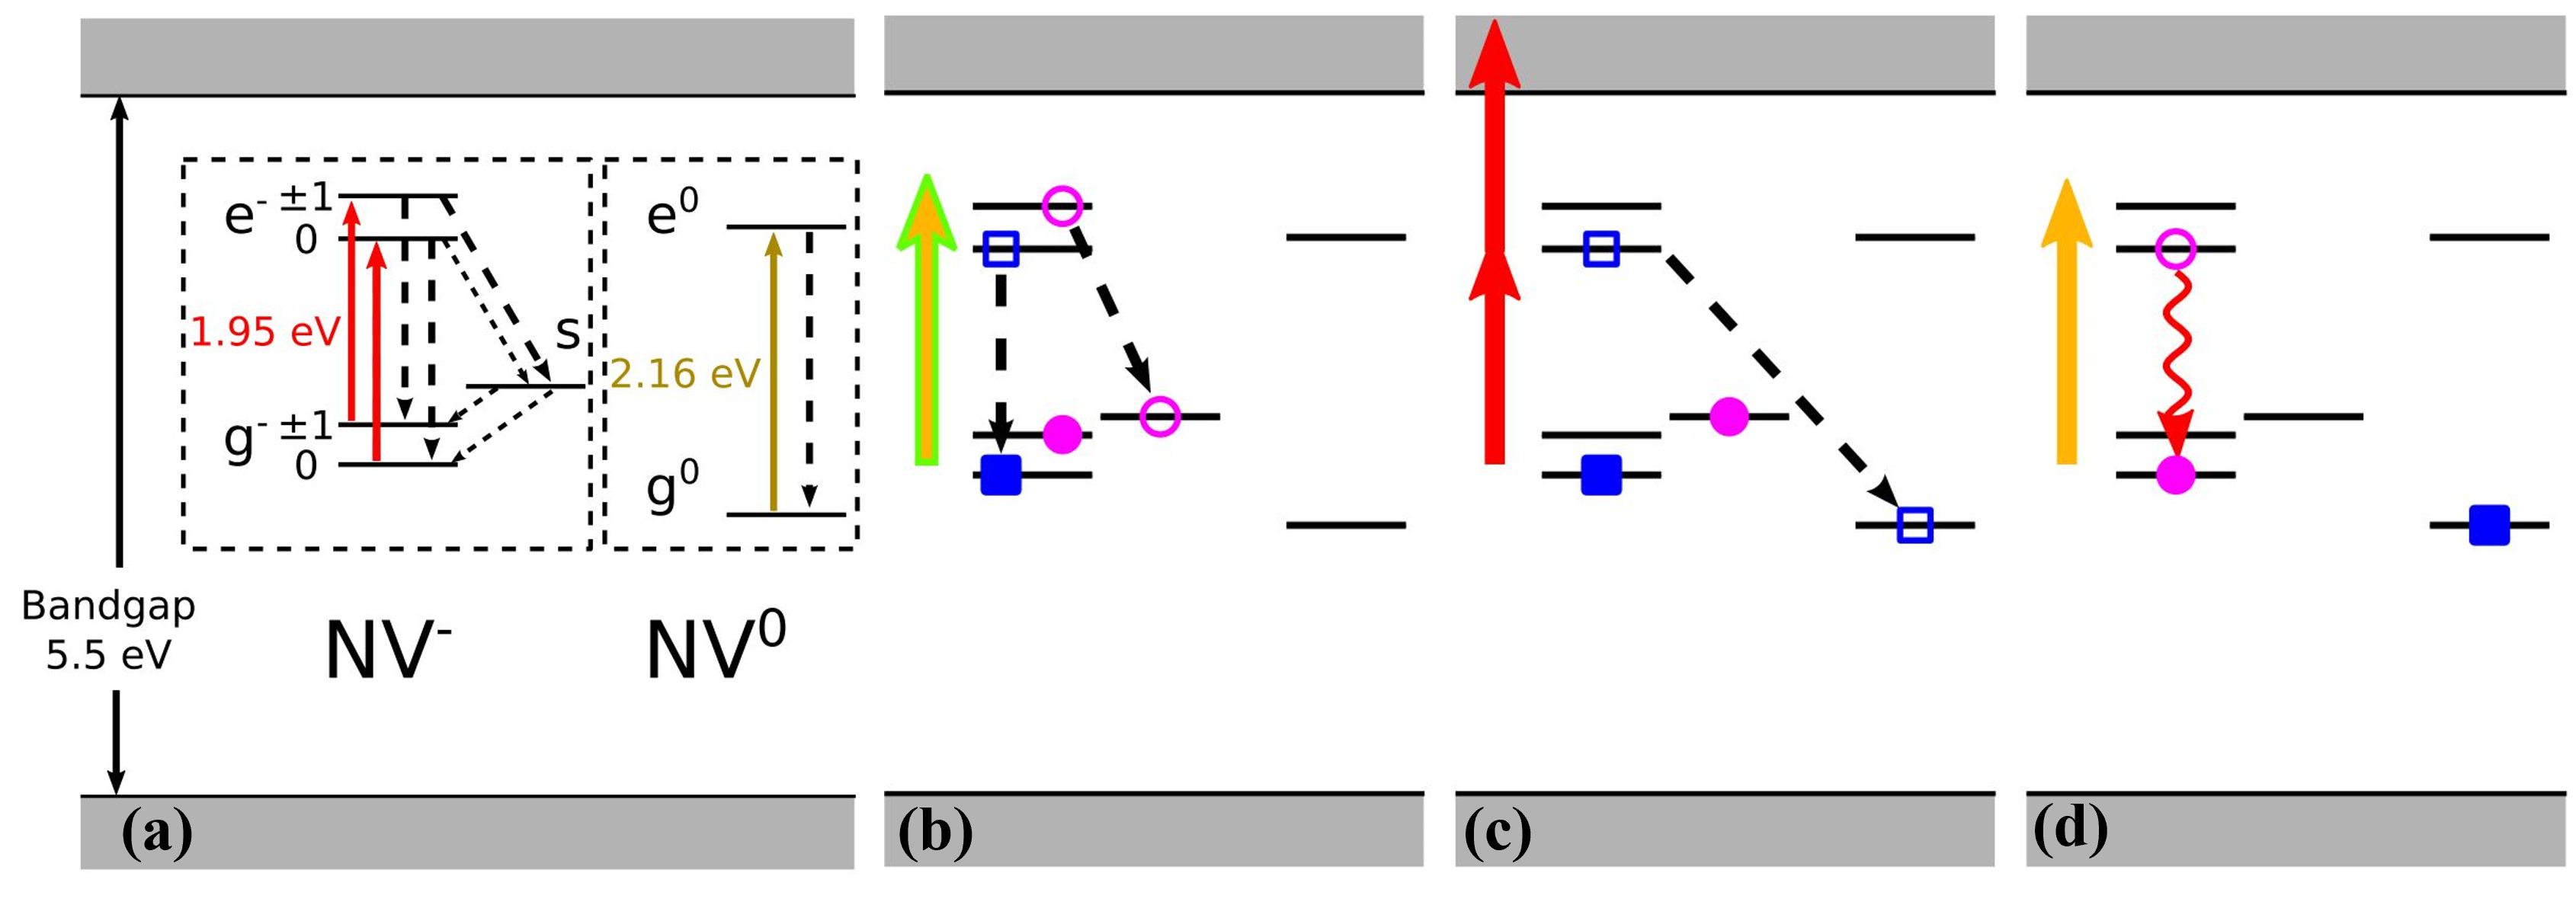
\includegraphics[width=1.0\textwidth]{figures/Chapter 3/Different Wavelength.png}
  \caption[NV$^-$和NV$^0$的电子能级结构和不同波长激光对于电子的调控]{NV$^-$和NV$^0$的电子能级结构和不同波长激光对于电子的调控,a、b、c分别是532 nm的绿光(或594 nm的黄橙光)、637 nm的红光、594 nm的黄橙光\cite{Shields2015}。}
  \label{fig: Different Wavelength}
\end{figure}

这些现象表明,NV Center的电荷态随着时间的变化并不是一个稳定的情况,而是有一个动态变化的状态,可以通过随着时间变化的相对电离和复合率来描述,这也是本文主要聚焦的问题。由于电离和复合的过程都可以用双光子过程来描述,因此在激光功率较低的时候,NV Center的荧光效应没有饱和前,电离和复合和激光光强有关,在后续的分析中需要考虑饱和光强这一限制因素。

除此之外,NV Center电荷态的电离和复合过程同样受到环境的影响,包括样品的晶体结构、掺杂等因素,以及环境温度、磁场、电场等实验环境因素,这些会在没有任何荧光效用的情况下影响NV Center的电荷态。比如,在制备样品的过程中,金刚石晶体中的一些缺陷结构会形成局域电子势阱(local electron traps),在NV$^-$转化为NV$^0$之后停止光学激发,电子将不会回落到NV Center缺陷能级附近,使得其变为暗态\cite{Bluvstein2019}。除此之外,一些施主掺杂元素在没有外界激发的激发的情况下,也会在一定程度上影响NV$^-$的布局数分布\cite{doi2016pure}。本人也曾利用基于第一性原理的密度泛函理论探究并证明了相比于实验中最为常见的氮元素施主掺杂的金刚石中的NV Center而言,磷元素施主掺杂的金刚石中的NV$^-$在保证其原有的量子比特的各种优异性质的同时,其NV Center的负电中心稳定性更强\cite{Zou2024}。

\section{NV Center电荷态动力学的理论模型}
在这一部分,本文将基于B. J. Shields和L. Hacquebard等人提出的方案,对于NV Center电荷态动力学的理论模型进行构建和分析\cite{Shields2015, Hacquebard2018}。NV Center的荧光发光特征可以通过在时间尺度记录APDs所收集到的单光子计数率来表征,当NV Center处于NV$^-$状态的时候,会有较高的计数率$\gamma_-$;当NV Center处于NV$^0$状态的时候,会有较低的计数率$\gamma_0$。$\gamma_-$和$\gamma_0$在本文后续都分别指代NV$^-$和NV$^0$的计数率,并用这两个可以直接探测到的参数在特定的读出时间(readout time)$t_r$区间下来构建收集到光子数结果的直方图。如果在一定的读出时间$t_r$之中,NV Center的电荷态没有发生改变,那这个可以用两个泊松概率分布函数(Poissonian Probability Distribution Functions, PPDF)来分别描述NV$^0$和NV$^0$态的布居数分布直方图:
\begin{equation}
  PPDF_0(n, \gamma_0 t_r) = \frac{(\gamma_0 t_r)^n exp(-\gamma_0 t_r)}{n!}
  \label{equ: PPDF_0}
\end{equation}
\begin{equation}
  PPDF_-(n, \gamma_- t_r) = \frac{(\gamma_- t_r)^n exp(-\gamma_- t_r)}{n!}
  \label{equ: PPDF_1}
\end{equation}
由于计数率的单位与时间相关,通常为kpcs/s(千光子每秒),而且荧光的光子在特定的读出时间中是随机的统计分布,也就是在自然情况下遵循泊松分布,即所以读取到特定电荷态计数率的均值为$\gamma_0 t_r$或$\gamma_- t_r$,作为泊松分布函数的变量,因此在一定的读出时间$t_r$之中,探测到的光子数量$n$的直方图可以计算:
\begin{equation}
P_{hist}(n)=P(NV^0)PPDF_0(n, \gamma_0 t_r)+P(NV^-)PPDF_-(n, \gamma_- t_r)
\end{equation}
其中$P(NV^0)$和$P(NV^-)$是在读出时间$t_r$的开始,NV Center处于特定电荷态的概率,两种状态的初始概率分别由单个泊松分布在总面积中占据的比例决定的。

然而,前文所讨论的NV Center缺陷电子能级结构中,未成对电子的电离和复合对应的电荷态的转换及其过程中的荧光效应的描述是一个简化模型,实际上电荷态在读出时间的尺度之内是极其不稳定的,可能会在这个时间段内发生数次电荷态的转换,这种电荷态转换可以用从NV$^0$到NV$^-$的复合率$g_{0-}$和从NV$^-$到NV$^0$的电离率$g_{-0}$这两个参数来描述。为了简单理解这样的电荷态动态转化的过程,可以用一些简单的例子来说明,如图 \ref{fig: Charge Conversion}a所示。在这个$t_r$的过程中,初始的电荷态为NV$^0$,持续时间为$\tau_1$,然后复合形成NV$^-$的概率为:
\begin{equation}
  p_1(\tau_1,g_{0-}) = g_{0-}\tau_1 \cdot e^{-g_{0-}\tau_1}
\end{equation}
这个式子为PPDF公式\ref{equ: PPDF_0}简单形式,其中$n=1$,$\gamma_0 = g_{0-}$,$t_r=\tau_1$。
同样的,对于序列的第二段和第三段而言,其概率为:
\begin{equation}
  p_2(t_1,g_{-0}) = g_{-0}t_1 \cdot e^{-g_{-0}t_1}
\end{equation}
\begin{equation}
  p_3(\tau_2,g_{0-}) = \tau_2 \cdot e^{-g_{0-}\tau_2}
\end{equation}
需要注意的是,我们假设在第三部分后,不会有电荷转换的情况产生,所以系数中不存在$g_{0-}$这一项。对于时间而言,有$\tau=\tau_1+\tau_2$和$t_r-\tau=t_1$,所以整体的概率为上述三个概率的乘积:
\begin{equation}
  \begin{aligned}
    P_a(\tau,t_r,g_{0-},g_{-0}) &= p_1 \cdot p_2 \cdot p_3 \\
    &= g_{0-}g_{-0}\tau_1\tau_2t_1 \cdot e^{(g_{-0}-g_{0-})\tau-g_{-0}t_r}
  \end{aligned}
\end{equation}
同样的,对于另外三种可能的情况,概率计算的结果如下:
\begin{equation}
  P_b(\tau,t_r,g_{0-},g_{-0}) = g_{-0}g_{0-}\tau_1\tau_2t_1 \cdot e^{(g_{0-}-g_{-0})\tau-g_{0-}t_r}
\end{equation}
\begin{equation}
  P_c(\tau,t_r,g_{0-},g_{-0}) = g_{0-}\tau_1t_1 \cdot e^{(g_{-0}-g_{0-})\tau-g_{-0}t_r}
\end{equation}
\begin{equation}
  P_c(\tau,t_r,g_{0-},g_{-0}) = g_{-0}\tau_1t_1 \cdot e^{(g_{0-}-g_{-0})\tau-g_{0-}t_r}
\end{equation}

\begin{figure}
  \centering
  \includegraphics[width=1.0\textwidth]{figures/Chapter 3/Charge Conversion.png}
  \caption[不同电荷初态时,NV Center电荷态的转换过程示意图]{不同电荷初态时,NV Center电荷态的转换过程示意图,观测的时间尺度为读出时间$t_r$, $\tau_i$为在$t_r$中和初始电荷态相同状态所持续的时间,$t_i$为在$t_r$中和初始电荷态不同状态所持续的时间。(a)初始电荷态为NV$^0$,且电荷态的转换次数为偶数;(b)初始电荷态为NV$^-$,且电荷态的转换次数为偶数;(c)初始电荷态为NV$^0$,且电荷态的转换次数为奇数;(d)初始电荷态为NV$^-$,且电荷态的转换次数为奇数。}
  \label{fig: Charge Conversion}
\end{figure}

在图 \ref{fig: Charge Conversion}中所展示的是在读出时间$t_r$中最基本的四种序列,分类依据是初始电荷态是NV$^-$或者NV$^0$以及电荷态转换的次数是奇数次或者偶数次。更一般的情况下,可以将这些情况进行组合,并且可能会有很多次的电荷态转换的现象产生,所以可以写出更为普适性的表达式,即对上面推导的式子分情况进行积分和求和:
\begin{equation}
  \begin{aligned}
    p(n|NV^0,even)=&\int_{0}^{t_r}d\tau e^{(g_{-0}-g_{0-})\tau-g_{-0}t_r} \sum_{i=1}^{\infty}(g_{0-}g_{-0})^i \prod_{j=1}^{i}\int_{0}^{\tau-\sum_{k=1}^{j-1}\tau_k}d\tau_j \\
    & \times \prod_{j=1}^{i-1}\int_{0}^{(t_r-\tau)-\sum_{k=1}^{j-1}t_k}dt_jPPDF(n, \gamma_0\tau+\gamma_-(t_r-\tau)) \\
    & + e^{-g_{0-}t_r}PPDF(n, \gamma_0t_r)
  \end{aligned}
\end{equation}
\begin{equation}
  \begin{aligned}
    p(n|NV^-,even)=&\int_{0}^{t_r}d\tau e^{(g_{0-}-g_{-0})\tau-g_{0-}t_r} \sum_{i=1}^{\infty}(g_{-0}g_{0-})^i \prod_{j=1}^{i}\int_{0}^{\tau-\sum_{k=1}^{j-1}\tau_k}d\tau_j \\
    & \times \prod_{j=1}^{i-1}\int_{0}^{(t_r-\tau)-\sum_{k=1}^{j-1}t_k}dt_jPPDF(n, \gamma_-\tau+\gamma_0(t_r-\tau)) \\
    & + e^{-g_{-0}t_r}PPDF(n, \gamma_-t_r)
  \end{aligned}
\end{equation}
\begin{equation}
  \begin{aligned}
    p(n|NV^0,odd)=&\int_{0}^{t_r}d\tau e^{(g_{-0}-g_{0-})\tau-g_{-0}t_r} \sum_{i=1}^{\infty}g_{0-}^ig_{-0}^{i-1} \prod_{j=1}^{i-1}\int_{0}^{\tau-\sum_{k=1}^{j-1}\tau_k}d\tau_j \\
    & \times \prod_{j=1}^{i-1}\int_{0}^{(t_r-\tau)-\sum_{k=1}^{j-1}t_k}dt_jPPDF(n, \gamma_0\tau+\gamma_-(t_r-\tau)) \\
    & + e^{-g_{0-}t_r}PPDF(n, \gamma_0t_r)
  \end{aligned}
\end{equation}
\begin{equation}
  \begin{aligned}
    p(n|NV^-,odd)=&\int_{0}^{t_r}d\tau e^{(g_{0-}-g_{-0})\tau-g_{0-}t_r} \sum_{i=1}^{\infty}g_{-0}^ig_{0-}^{i-1} \prod_{j=1}^{i-1}\int_{0}^{\tau-\sum_{k=1}^{j-1}\tau_k}d\tau_j \\
    & \times \prod_{j=1}^{i-1}\int_{0}^{(t_r-\tau)-\sum_{k=1}^{j-1}t_k}dt_jPPDF(n, \gamma_-\tau+\gamma_0(t_r-\tau)) \\
    & + e^{-g_{-0}t_r}PPDF(n, \gamma_-t_r)
  \end{aligned}
\end{equation}
这四个通用公式是由M. D. Lukin及其团队在2015年提出的,用以解释电荷态在一定的读出时间内转换的普适性概率模型 \ref{shields2015efficient}。由这个公式,我们可以得到在这个读出时间段内光子数$n$的直方图计算表达式:
\begin{equation}
  \begin{aligned}
    P(n)&=P(NV^0)[p(n|NV^0,even)+p(n|NV^0,odd)] \\
    &+P(NV^-)[p(n|NV^-,even)+p(n|NV^-,odd)] \\
    &=P(NV^0)p(n|NV^0)+P(NV^-)p(n|NV^-)
  \end{aligned}
\end{equation}
由这个式子可以得到,在这个模型中,只剩下初始态处于NV$^0$或NV$^-$的概率$P(NV^0)$和$P(NV^-)$需要来确定,由此我们需要进行连续波(continuous wave)和脉冲(pulsed)测量来分布确定所需要的数据,这里的连续波和脉冲测量指的是在读出时间内激光是否会间断。

\subsection{CW测量下初始电荷态分布和读出保真度}
一旦知道了电荷态转换率$g_{-0}$和$g_{0-}$,电荷态动力学分布就可以用下面两个微分系统方程来描述:
\begin{equation}
  \dot{\rho}_- = g_{0-}\rho_0-g_{-0}\rho_-
  \label{equ: differential equations_-}
\end{equation}
\begin{equation}
  \dot{\rho}_0 = -g_{0-}\rho_0+g_{-0}\rho_-
  \label{equ: differential equations_0}
\end{equation}
其中$\rho_-$是负电荷态总体概率分布,而$\rho_0$是中性电荷态总体分布的概率,即:
\begin{equation}
  P(NV^-) \equiv \rho_-
\end{equation}
\begin{equation}
  P(NV^-) \equiv 1-\rho_- = \rho_0
\end{equation}
然而,在恒定功率和波长的激光CW激发测量下,系统中的电荷态是近乎稳定,也就是$\dot{\rho}_0 = \dot{\rho}_- = 0$,因此由式\ref{equ: differential equations_-}和\ref{equ: differential equations_0}可以得到:
\begin{equation}
  \frac{g_{0-}}{g_{-0}}=\frac{\rho_-}{\rho_0}
\end{equation}
\begin{equation}
  P(NV^-)=\frac{g_{0-}}{g_{0-}+g_{-0}}
\end{equation}
通过这些计算,可以构建利用CW测量电荷态的模型和实验方案。

另外一个比较重要的特征是我们可以通过CW测量来得到读出保真度$\mathcal{F}_C$,也就是我们能够顺利读出并正确判断电荷态的可信度。其中一个关键点是设定一个合适的光子计数率阈值$n_{thresh}$来区分NV$^0$和NV$^-$的分布状态。因为NV$^0$状态时的计数率要远低于NV$^-$,所以在一定的读出时间$t_r$之中,如果计数率低于$n_{thresh}$,则计入NV$^0$的部分,反之则计入NV$^-$的部分。读出效率的公式可以由此计算:
\begin{equation}
  \mathcal{F}_c = \frac{1}{2}[\sum_{n=0}^{n_{thresh}}p(n|NV^0)+\sum_{n_{thresh}}^{n_{max}}p(n|NV^-)]
\end{equation}
我们需要最大化读出效率,所以需要对于读出594 nm橙光的功率$P$和读出时间$t_r$进行测试和优化,从而使得$\mathcal{F}_C$达到尽可能大的数值,这对于基于单次读出激光来收集统计光子数的单次读出(single shot readout)技术而言非常重要。

除此之外,区分NV$^0$和NV$^-$的阈值$n_{thresh}$的设定同样十分重要。如图 \ref{fig: n_thresh}所示,左图(a)为实验中利用APDs测得的原始数据,展示了在读出时间$t_r$中不同时刻计数率的变化曲线,我们可以很明显可以看到,在其中计数率高的为NV$^-$,计数率低的为NV$^0$。而右图(b)则是将(a)图中的计数率转化为其概率密度分布的直方图,可以看到由明显的两个峰值,然后用两个泊松概率分布函数进行拟合,从而得到了两种电荷态的曲线,左边整体计数率低的峰的拟合曲线表示的是NV$^0$,右边整体计数率高的峰的拟合曲线表示的是NV$^-$,这两条曲线有一个交点,通常将这个交点设置为$n_{thresh}$来区分两种不同的电荷态,并用于计算读出保真度$\mathcal{F}_C$。

\begin{figure}
  \centering
  \includegraphics[width=1.0\textwidth]{figures/Chapter 3/n_thresh.png}
  \caption[计数率的统计和$n_{thresh}$的确定]{计数率的统计和$n_{thresh}$的确定,(a)图中展示了APDs计数率随着时间的变化趋势,(b)中的柱状图展示了讲计数率转化为概率密度分布的曲线\cite{Aslam2013}。}
  \label{fig: n_thresh}
\end{figure}

\subsection{脉冲测量中初始化电荷态和初始化保真度$\mathcal{F}_I$}
当进行脉冲序列测量的时候,电荷态将不会保持一个稳定的状态,而是会随着初始化脉冲和读出脉冲的序列而发生变化。为了初始化电荷态,即将尽可能多的NV$^0$转化到NV$^-$的$m_s=0$态,在594 nm的橙光读出后,会紧跟着一束持续3000 ns的高功率532 nm的绿光脉冲来对NV Center进行初始化。这种方法的原理是基于不同波长的激光会对NV Center的电荷和复合产生比较大的影响。在532 nm的绿光脉冲的作用下,NV$^0$的电子会被激发到更高的能级,从而能和价带中或者电子势阱中的额外电子结合,使得NV Center回到NV$^-$的状态,而NV$^-$在基态三重态$m_s=±1$的电子则会被激发到NV$^-$的激发态,然后通过ISC过程回到NV$^-$的$m_s=0$基态,这样就使得NV Center被初始化。

脉冲测量的主要作用就是确定初始化保真度$\mathcal{F}_I$,而在施加绿光脉冲的过程中,NV$^-$的电离作用主要取决于绿光的功率,也就是说功率过高的绿光会将NV$^-$再次电离,这样就会降低电离的保真度,所以需要对于绿光的功率进行优化,使得初始化保真度$\mathcal{F}_I$达到最大值。$\mathcal{F}_I$可以通过随着时间变化的计数率直方图来计算,通过拟合初始的光子数来得到:
\begin{equation}
  P(n)_{ini}=(1-\mathcal{F}_I)p(n|NV^0)+\mathcal{F}_Ip(n|NV^-)
\end{equation}
其中$p(n|NV^0)$和$p(n|NV^-)$分别是NV$^0$和NV$^-$的概率分布,而$\mathcal{F}_I$则是初始化保真度,即初始化NV$^0$为NV$^-$的概率。在这个模型中,我们假设了在初始化脉冲之后,NV Center的电荷态不会发生改变,即在读出脉冲之前,NV Center的电荷态不会发生改变,这个假设在实验中是成立的,因为初始化脉冲的时间尺度远小于读出脉冲的时间尺度,所以在读出脉冲之前,NV Center的电荷态不会发生改变。

对于初始化保真度的优化同样十分重要,因为初始化脉冲在大部分涉及到NV Center的实验中,通常被用于在测量序列之前让尽可能多的NV Center转化为方便调控和读出的NV$^-$,并且提高NV Center用于量子信息领域时候较为重要的自旋相干时间这一参数\cite{Robledo2011}。

\end{document}
\documentclass[type = bachelor, oneside]{whu-thesis}
\usepackage{textcomp,mathcomp}
\usepackage{siunitx}
\usepackage{chemfig}
\usepackage{graphicx}

\whusetup
  {
    info               =
      {
        title          = {金刚石氮-空位色心的\\电荷态调控和性质表征},
        title*         = {Modulation of Charge States and Characterization of Properties\\ in Nitrogen-Vacancy Centers of Diamond},
        student-number = {2020302192129},
        school         = {弘毅学堂},
        author         = {邹迪玮},
        author*        = {Diwei Zou},
        subject        = {学科},
        major          = {微电子科学与工程},
        advisor        = {周利 , 副教授;孙启超 , 研究员},
        direction      = {研究方向},
        date           = {2024/5},
        keywords       = {关键词 1 , 关键词 2 , 关键词 3 , 关键词 4 , 一个非常非常,非常非常长——的关键词 5},
        keywords*      = {key word 1 , key word 2 , key word 3 , key word 4 , {and a very very, very very long key word---the key word 5}},
      },
    style              =
      {
        graphics-path  = {{figures/}{data/}},
        list-of-figures,
        list-of-tables,
      },
    element            =
      {
        innovation     = {pages/innovation},
        abstract       = {pages/abstract},
        abstract*      = {pages/enabstract},
        bibliography   = {ref/refs_all}
      }
  }
\begin{document}

% Chapter 4

\chapter{实验平台的设计与搭建}

\section{共聚焦显微镜光学系统实验平台}
\subsection{共聚焦显微镜的基本原理}
实验室中常见的光学显微镜是通过光源发出自然光(白光)投射到被测样品上,样品的反射或透射光被物镜聚焦到目镜上,通过目镜观察到被测样品的图像。这种显微镜的分辨率受到可见光的波长的限制,通常在0.2 $\mu m$左右。为了提高显微镜的分辨率,人们提出了共聚焦显微镜(Confocal Microscopy)的概念,通过在显微镜中加入共聚焦系统,可以使得显微镜的分辨率提高到0.1 $\mu m$以下。共聚焦显微镜的基本原理是通过激光光源发出的激光束照射到样品上,样品的受到激光的激发后,在退激发的过程中会产生荧光效应释放出光子,被物镜聚焦到探测器上,并将信息传回到电脑。共聚焦显微镜的分辨率受到激光波长和物镜规格的限制,通常能在0.1 $\mu m$以下。共聚焦显微镜的优点是可以观察到样品的表面形貌和内部结构,实现三维的成像,非接触式无损的高分辨率、高灵敏度、高对比度的观察。

对于NV Center而言,由于基态能级结构的电子能被绿光激发,并在退激发的过程中发射声子边带的红光光子,所以共聚焦显微镜的原理可以用于对金刚石中的NV Center进行表征和检测,通过激光的聚焦和荧光的检测,可以实现对不同深度NV Center的三维定位和成像。一般来说,共聚焦显微镜有以下几个主要的部分:激光光源、激光束聚焦系统、样品台、物镜、探测器、数据采集系统等等。平台的构建也有多种方案,通过镜头的放置方式和扫描的运行方式来区分。
\begin{figure}
  \centering
  \includegraphics[width=0.8\textwidth]{figures/Chapter 2/Confocal Platform.png}
  \caption[共聚焦显微镜平台]{共聚焦显微镜平台,样品放置于手动XYZ三轴位移台上进行粗调节和聚焦,显微物镜倒置放置于压电纳米XYZ三轴位移台上进行精细扫描和聚焦。微波利用同轴线缆传递到样品表面,磁体也通过三轴手动位移台调节与样品的相对位置。}
  \label{fig: Confocal Platform}
\end{figure}
如图 \ref{fig: Confocal Platform}所示,我们采用的方案是镜头倒置,通过纳米压电位移台移动镜头对样品表面进行扫描的方案。压电位移台为XYZ三轴位移台,移动范围均为100 $\mu m$,精度和稳定性为10 nm的量级,可以实现亚微米级别的扫描和定位。如图 \ref{fig: Confocal Optimizer}所示,展示了Confocal显微镜的Optimize图像,左图为XY方向二维扫描的图像,用于确定NV Center在二维平面的位置;右图为Z方向扫描在不同深度的计数率,用于确定NV Center的深度。我们通过使用的德国Ulm University科研人员开发的基于Python的开源软件Qudi来对整套共聚焦系统进行控制,其中的Optimize功能能够在指定范围内自动寻找计数率高的位置来聚焦寻找NV Center,即图 \ref{fig: Confocal Optimizer}所示效果 \cite{Binder2017}。用于测试的样品的NV Center是通过在Element Six公司生产的电子级金刚石表面注入$^{14}$N离子形成的,所以NV Center的位置大部分在离表面5 $\mu m$内的浅层位置,使其发射的荧光光子能够尽可能多的被物镜所接收,提高实验数据和结果的对比度。
\begin{figure}
  \centering
  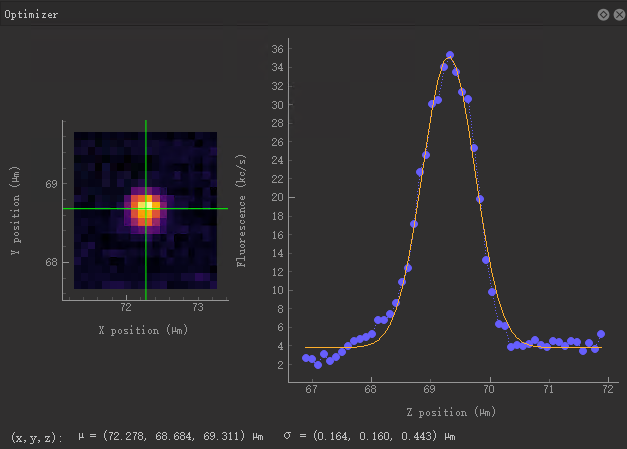
\includegraphics[width=0.6\textwidth]{figures/Chapter 2/Confocal Optimizer.png}
  \caption[Confocal显微镜的扫描和Auto Optimize功能]{Confocal显微镜的扫描和Auto Optimize功能。}
  \label{fig: Confocal Optimizer}
\end{figure}

\subsection{共聚焦显微镜的搭建}
如图 \ref{fig: Light Path}展示了实验中的光路简图,其中画出了主要元件,一些用于微调调整光路的普通透镜、反射镜、光阑等原件并未画出。对于532 nm的绿光光路而言,激光器产生的激光在出口处耦合进通过光纤输出,光纤用法兰连接光纤声光调制器(Acousto-Optic Modulator,AOM),经过AOM后在通过光纤输出,并在光纤末端用准直器将激光聚焦为高斯光束。AOM是一种通过压电声学效应改变晶体衍射效应,从而对光信号进行调制的器件。我们使用的AOM的驱动器有模拟和数字两个输入口,通过模拟信号输入不同的电压(0-5 V),可以对光强大小进行无级调节;而利用任意波形发生器(Arbitrary Waveform Generator,AWG)产生高频的高低电平,输入给AOM驱动器的数字接口,则可以实现对激光的快速开关,实现特定序列的脉冲测量,其上升沿和下降沿大约为400 ns。激光输出后,通过一个9:1的消偏振分光棱镜(Non-Polarizing Beam Splitter,NPBS),将透射光和反射光的光强分为9:1的两份,且没有改变偏振方向。经过NPBS后,90 \%的透射光透过NPBS继续在光路中传播,而剩下10 \%的反射光则被光电二极管(Photodioad,PD)收集,将光强成比例地转化为电流通过一个定值电阻,通过测量其两端的电压来实时监测光强的大小。经过NPBS的透射光继续传播,穿过550 nm和600 nm截止波长的两个低通二项色镜(Low Pass Dichroic Mirror,LP DM),通过压电位移台设计的孔洞中进入物镜,聚焦于样品表面。前文中有提到过NV Center会受到532 nm的绿光激发后,退激发的过程中发出637 nm的ZPL和波长更长的PSB,这些荧光被同一个物镜收集并原路返回,这些荧光在遇到600 nm LP DM后被反射向左,经过一个663-800 nm的带通滤波片(Band Pass Filter,BP Filter)后,大部分PSB进入单光子雪崩二极管(Avalanche Photodiode,APD)收集,每次收集到一个光子后就会形成脉冲信号,并将数字信号传递给电脑。
\begin{figure}
  \centering
  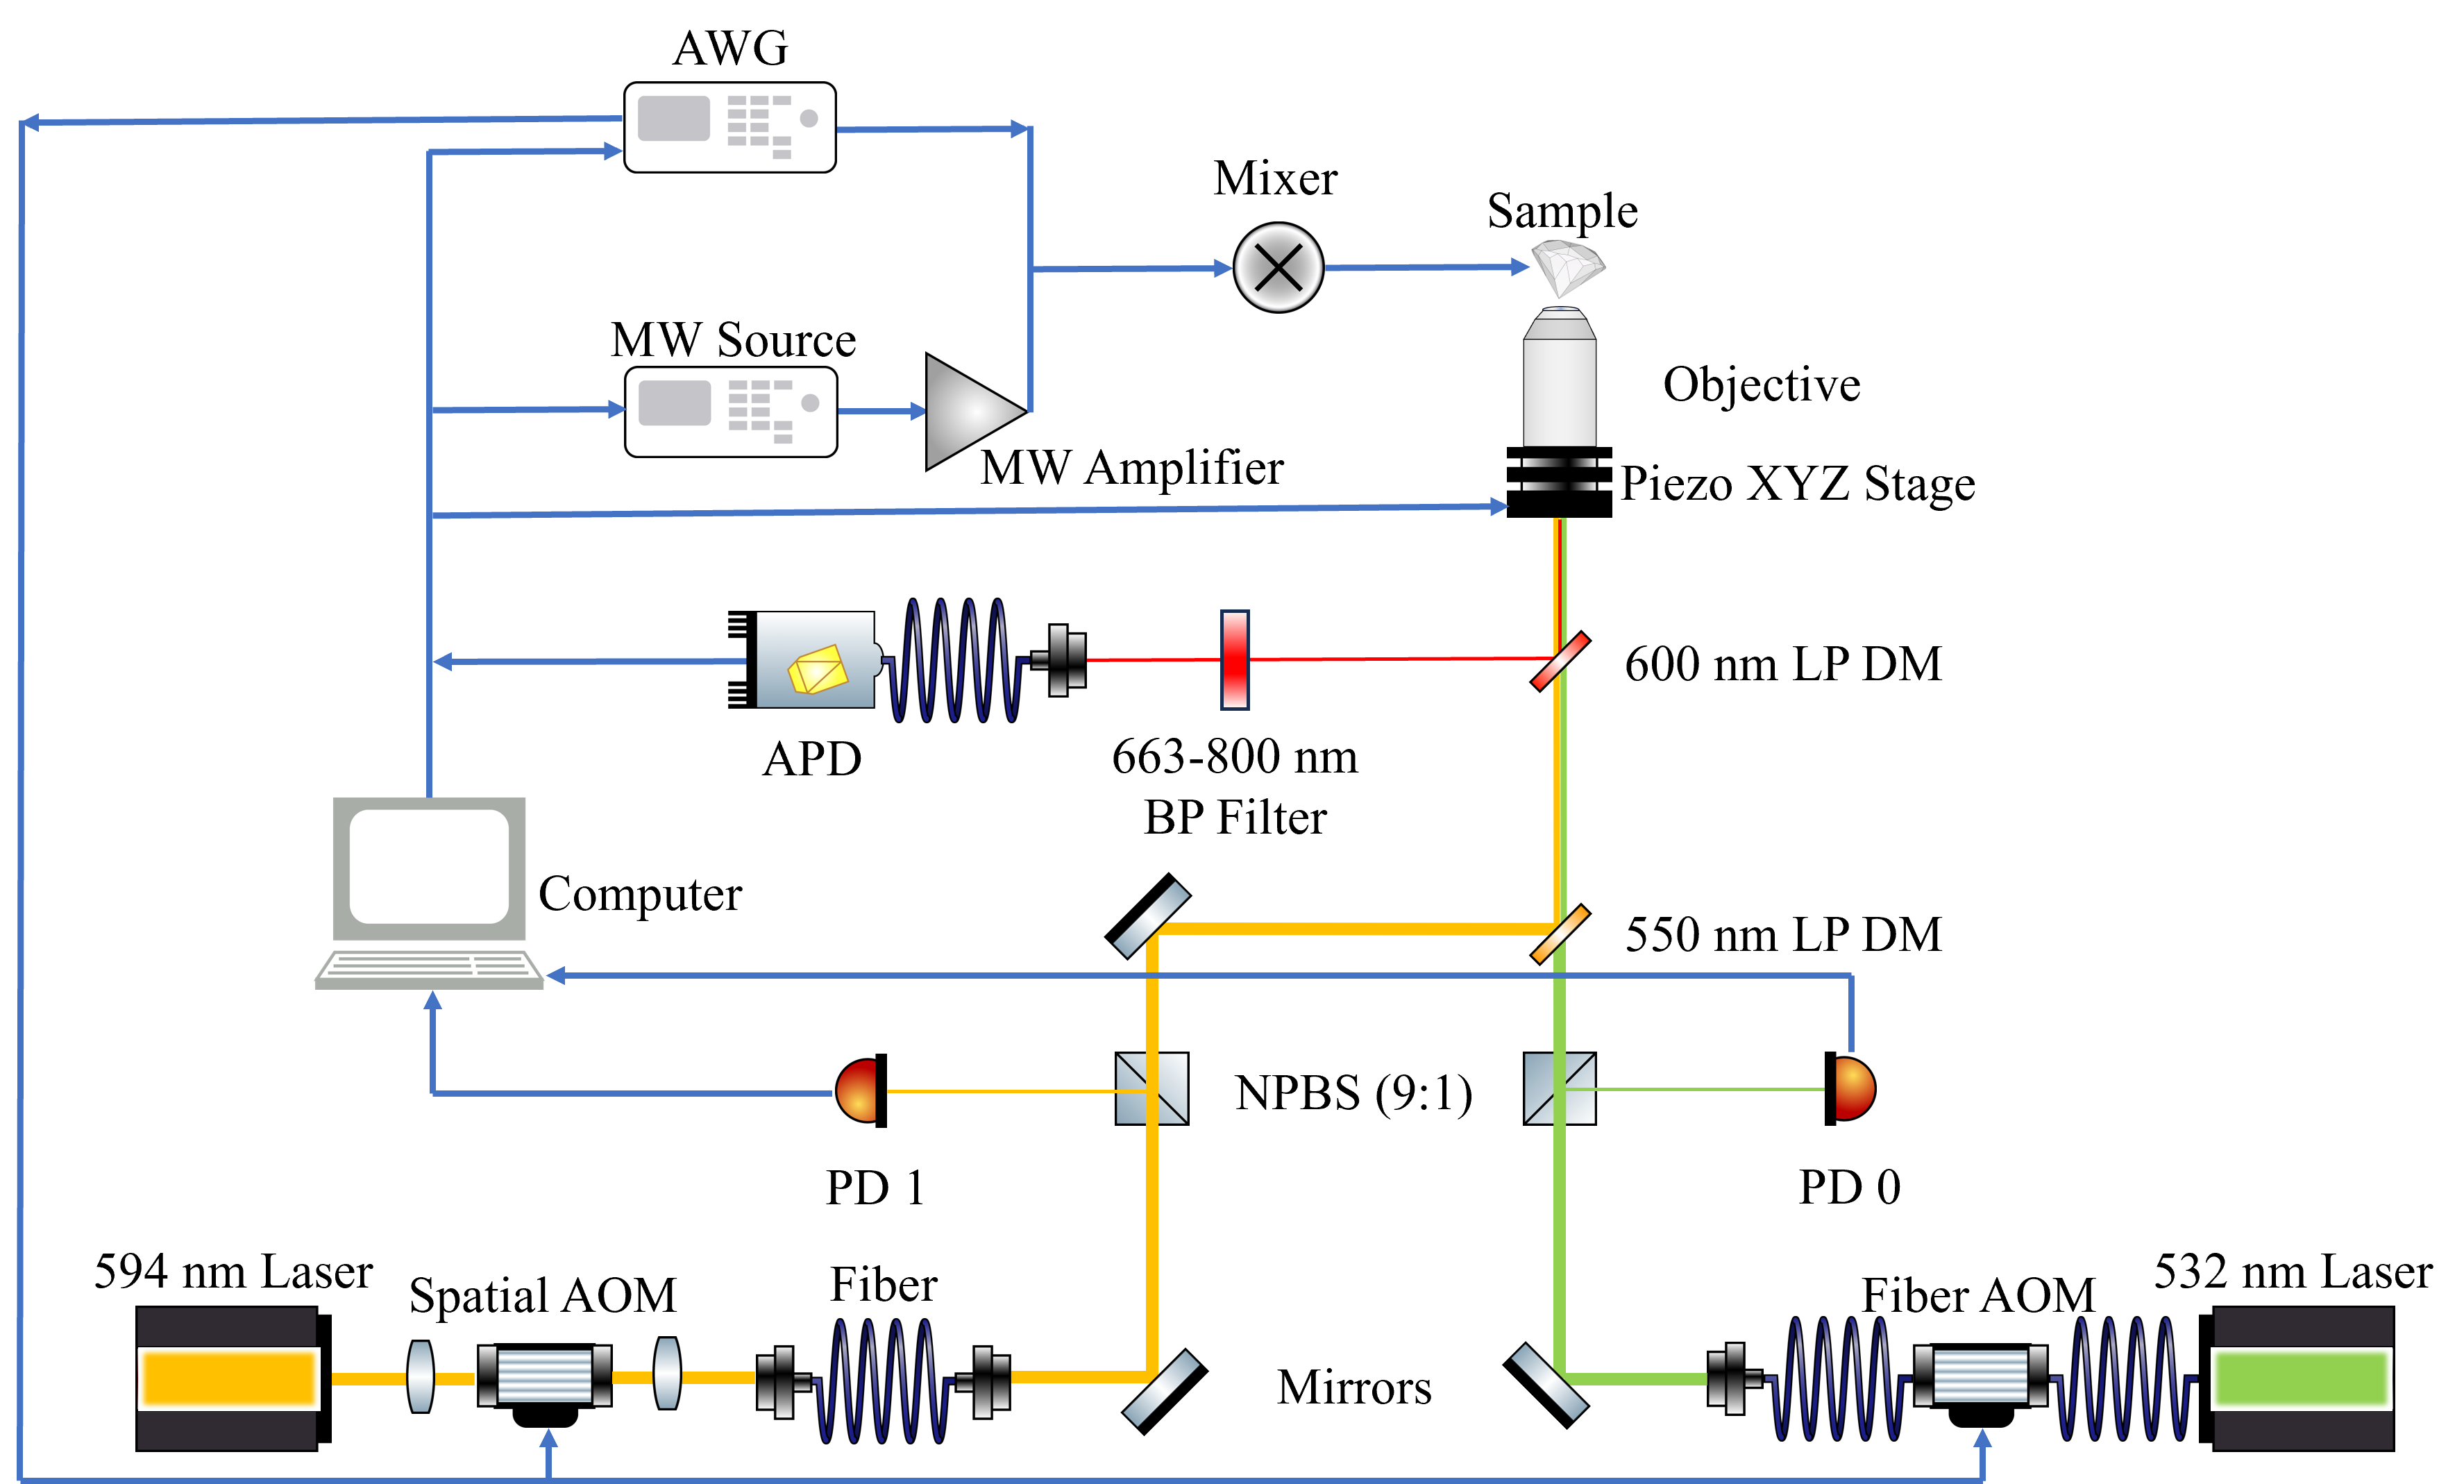
\includegraphics[width=1.0\textwidth]{figures/Chapter 2/Light Path.png}
  \caption[共聚焦显微镜光路简图]{共聚焦显微镜光路简图。}
  \label{fig: Light Path}
\end{figure}

对于594 nm的橙光光路而言,大部分的设计与532 nm的绿光光路相似,有一点不同的是这个光路中应用的AOM是空间AOM,激光以空间光的形式,通过一个透镜聚焦进入AOM,在出口处相同位置处放置一个相同焦距的透镜来将光束准直。激光经过空间AOM后,会形成多级衍射光斑,其中一级和负一级衍射光斑是可以通过控制AOM来进行调制的,因此我们利用光阑过滤掉了其他光斑,仅留下了一级衍射光斑在光路中继续传播。由于高斯光束在经过AOM后的形状会变得畸形,所以通过物镜耦合进入光纤传递来进行整形,再通过物镜和五维光纤调整架进行准直。如图 \ref{fig: 594 Collimator}所示,通过调整光纤头的位置,对准物镜的出口,准直的高斯光束会从物镜入口处反向射出。由于594 nm的橙光和532 nm的波长不同,导致相差的微小差异,这套装置实际上相当一个可调焦距的准直镜头,将两束激光聚焦于同一平面内。随后,594 nm的橙光通过550 nm LP DM和532 nm的绿光耦合到一起共轴共线,进入显微物镜从而聚焦于样品表面。
\begin{figure}
  \centering
  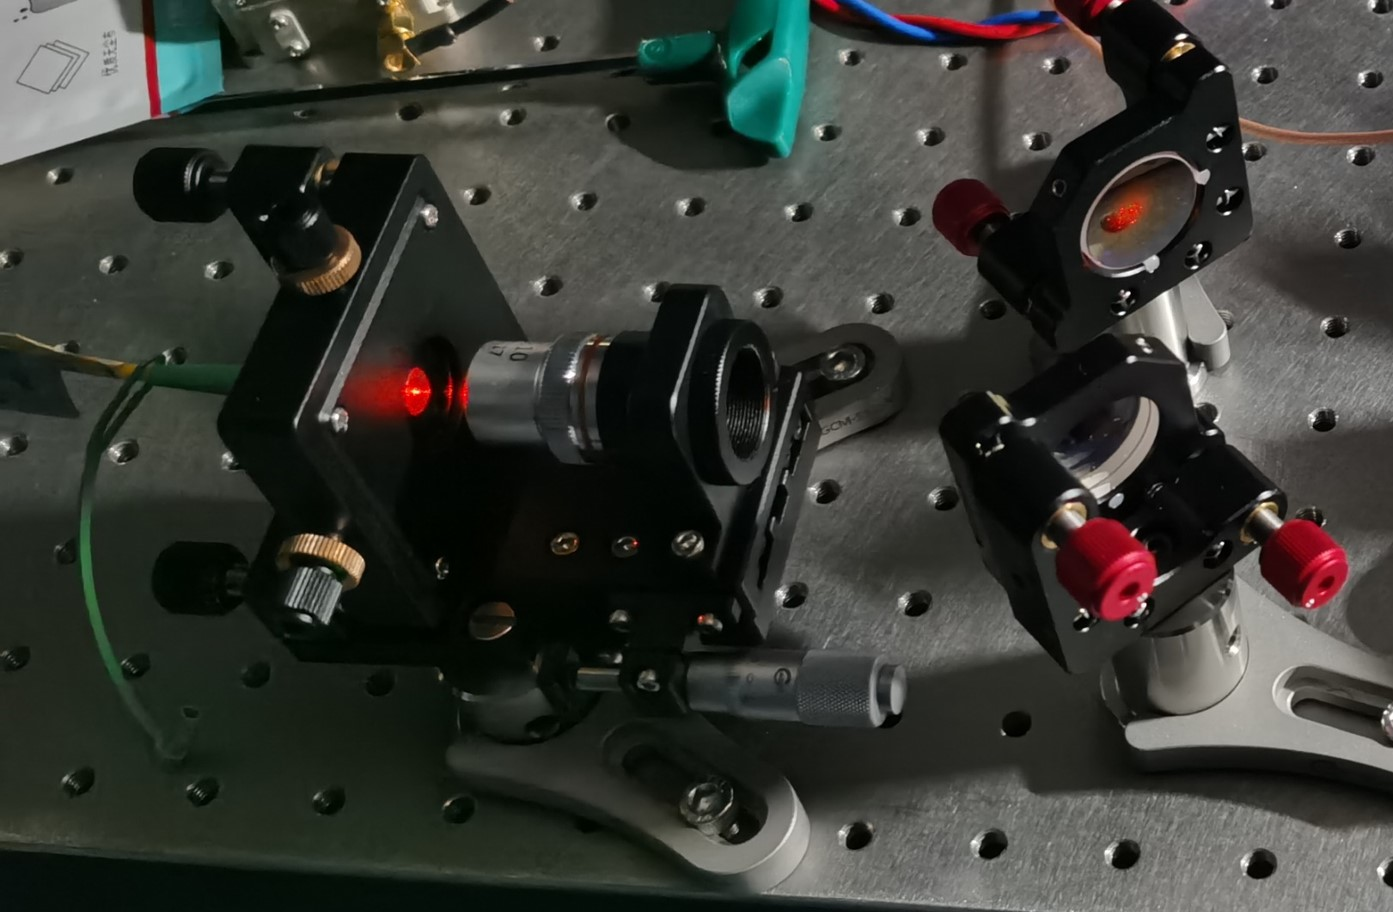
\includegraphics[width=1.0\textwidth]{figures/Chapter 2/594 Collimator.jpg}
  \caption[594 nm光纤光束准直]{594 nm光纤光束准直,通过物镜和五维光纤调整架对激光进行准直。}
  \label{fig: 594 Collimator}
\end{figure}

\subsection{金刚石样品}
如图 \ref{fig: Sample}所示,样品被粘在铝合金转接板上,转接板和电路板通过蓝色的铝合金螺丝固定,放置铁磁性材料的磁场干扰,或者再施加磁场的过程中受力而发生位移。电路板两头为SMA射频连接头,一头连接混频器发射的微波信号,另一头连接50 $\Omega$的阻抗衰减。中间贯穿的条带为导线,两侧铺铜接地隔离将电磁场束缚在中心,中间部分焊接一根50 $\mu m$粗的铜线作为微波天线,紧贴样品表面使微波在样品表面辐射。微波源(Microwave Source,MW Source)的信号经过放大器,通过混频器(Mixer)和AWG的信号混合后,通向样品电路板的SMA射频连接头。混合AWG信号的目的是在原有设置的恒定的GHz量级的微波信号基础上,加上一个MHz量级的射频信号,从而实现更精细的Pulsed ODMR测量。图中在混频器后省略了微波开关,其功能是通过AWG控制微波的通断来进行特定的序列测量,比如FID、Rabi Oscillation、Hahn-echo Sequence等。
\begin{figure}
  \centering
  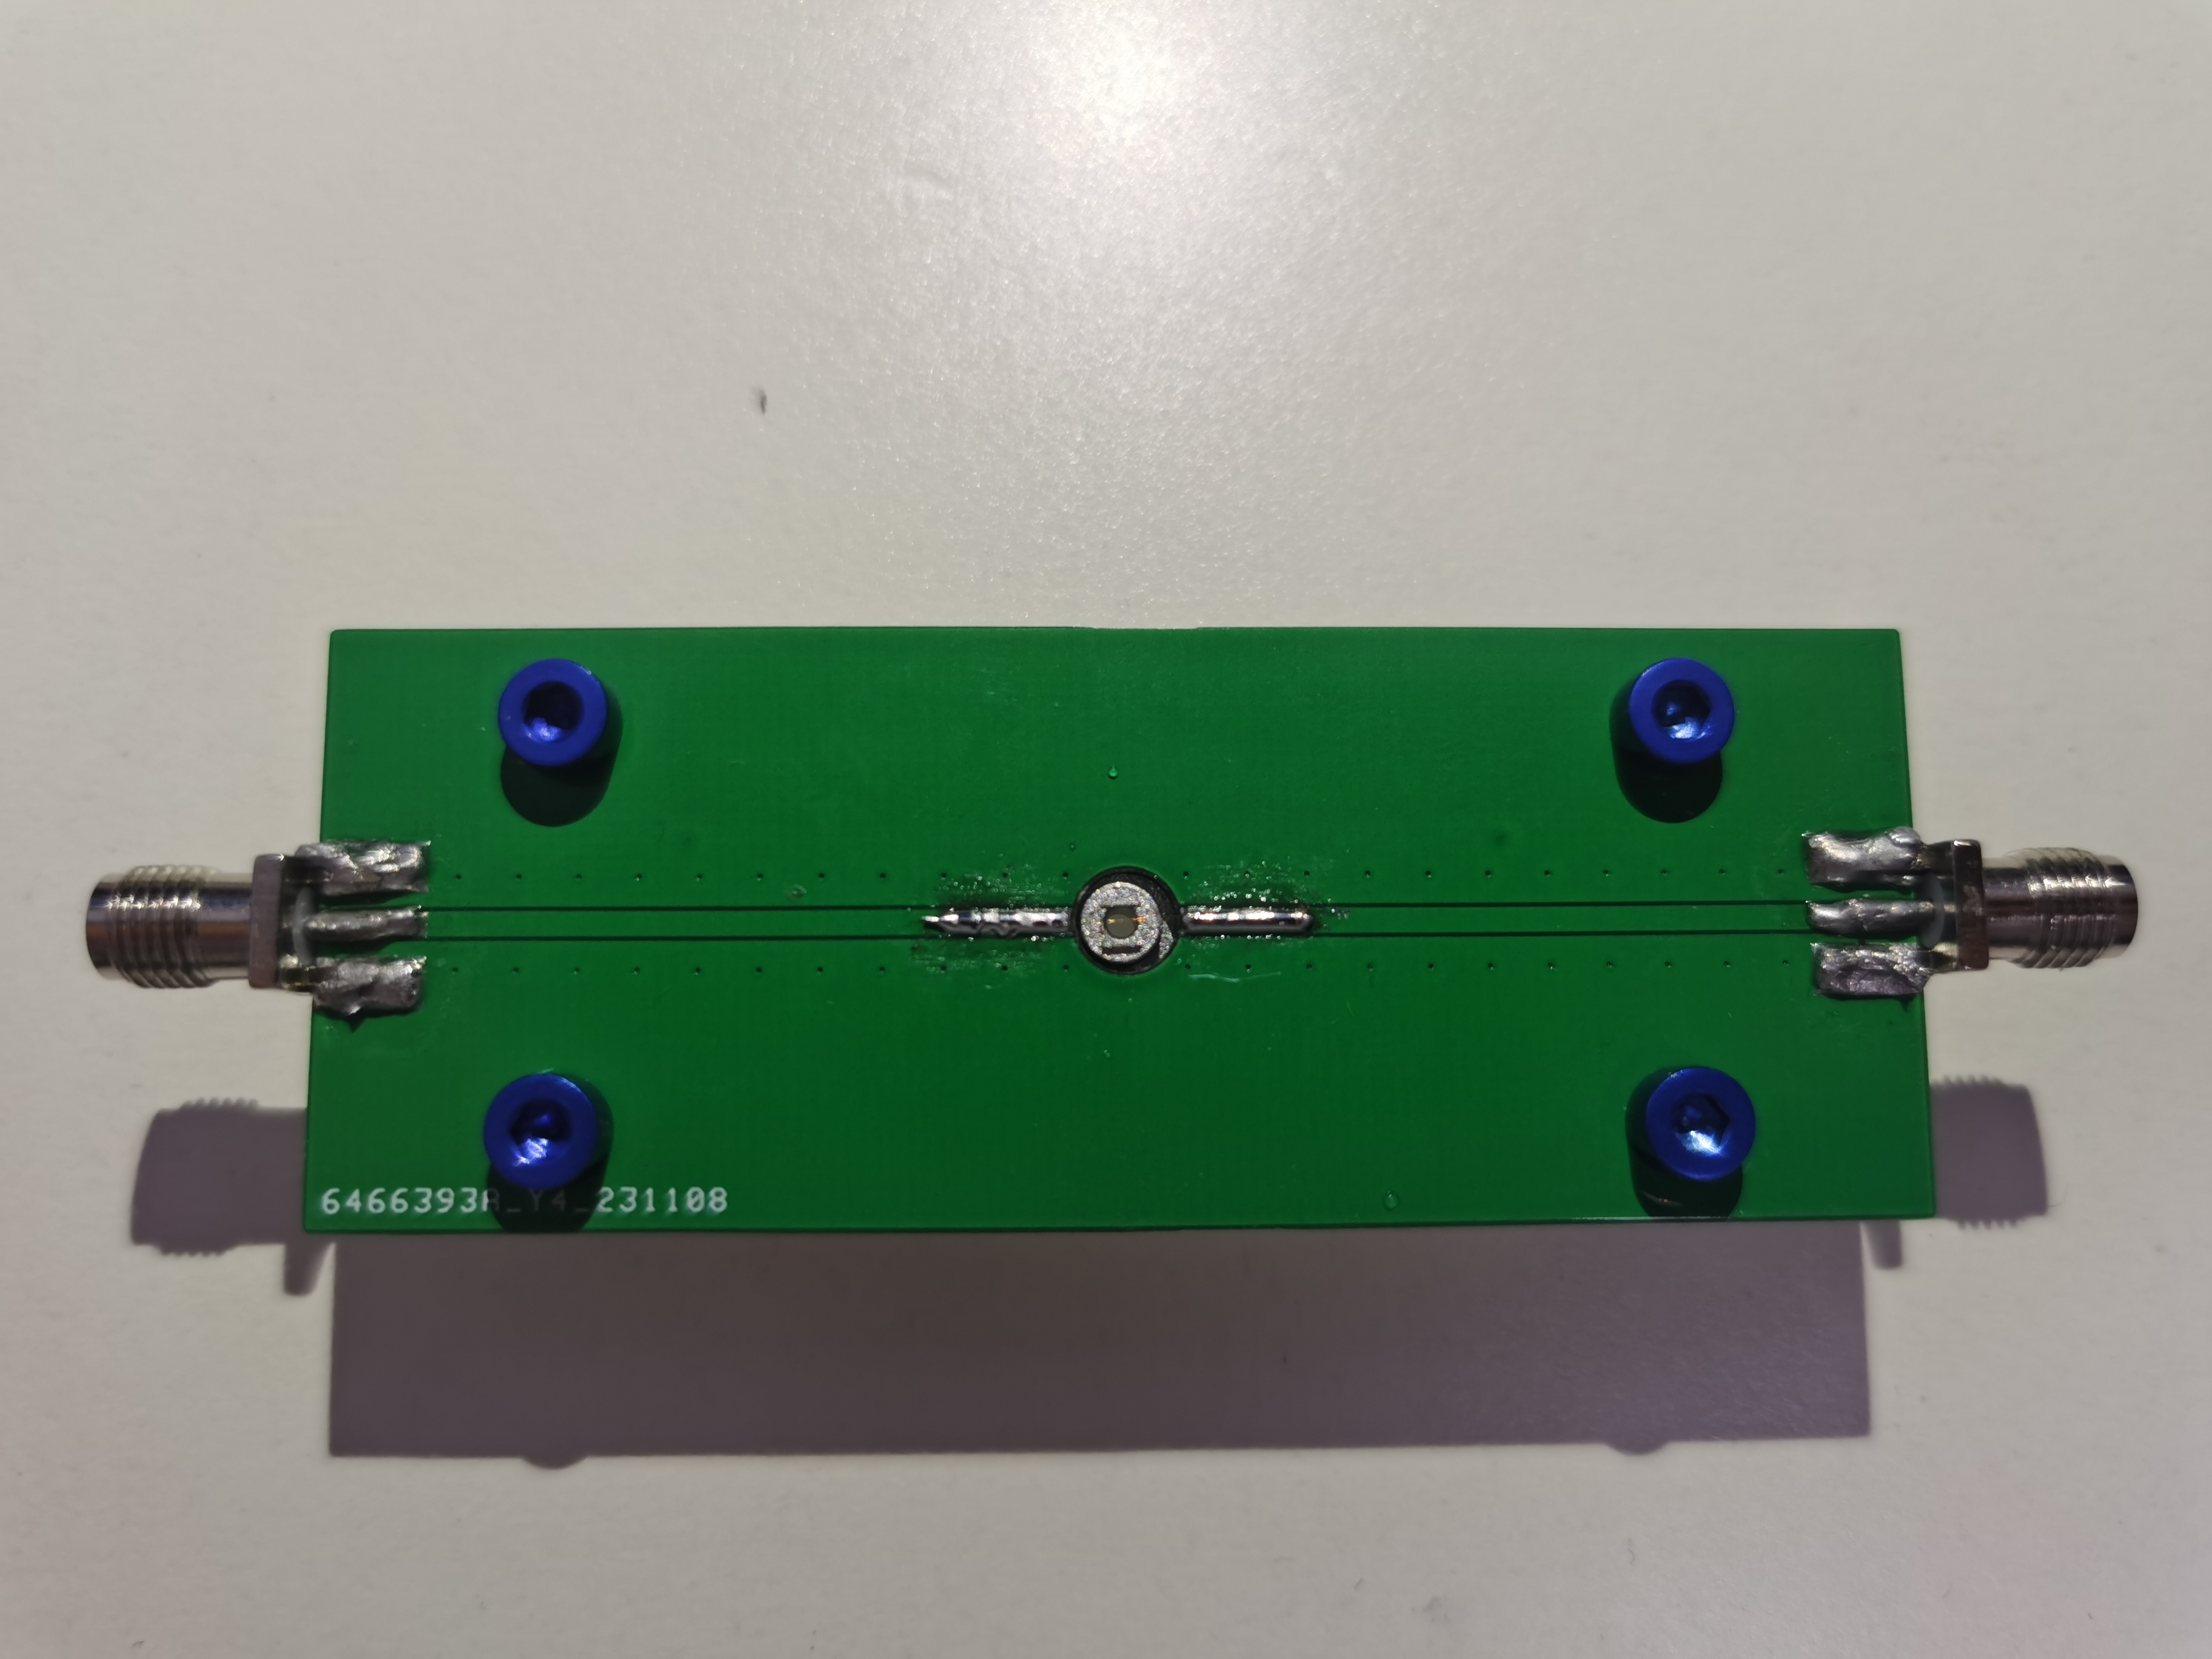
\includegraphics[width=1.0\textwidth]{figures/Chapter 2/Sample.jpg}
  \caption[金刚石样品和微波天线结构]{金刚石样品和微波天线结构。}
  \label{fig: Sample}
\end{figure}

\section{测量过程的设计}
\subsection{数据的采集过程}
在测量的过程中,我们选取了两个序列,分别为连续波序列(Continuous Wave,CW)和脉冲序列(Pulsed)两种形式,CW Measurement的目的是为了检测NV Center的电荷态动态平衡分布情况,而Pulsed Measurement的目的是为了将调控电荷的分布并且将自选转化为电荷态进行表征。在整个过程中,我们需要记录的数据只有时间尺度下的荧光发射光子数。在这个过程中,我们利用了时间标记器(Time Tagger,TT),也就是一种基于Opal Kelly FPGA板卡编程设计和开发的时间数字转换器(Time-to-Digital Converter,TDC),可以记录ns级分辨精度的数字信号数据,用于将左右设备的时序逻辑同步对应。我们将AWG和APD的输出都接入到TT上,通过AWG输出序列来控制TT的计数器触发和记录序列,TT接收到高电平的触发信号后,在设定的记录序列接口处于高电平状态的时候就会持续记录数据。与此同时,将AWG连接控制532 nm绿光和594 nm的橙光AOM驱动器,以及微波开关,由此可以通过AWG控制生成的序列来控制激光快速精准的通断和微波的脉冲。这样我们就可以通过控制AWG的输出信号来实现对NV Center的操控和测量。

在准备阶段,我们可以在启动TT的时候设置每一轮测量的最小时间分辨率和整体的时间尺度,以及与物理接口所对应的信号收集通道、触发接口通道和测量脉冲序列通道。在后续的测量过程中,我们设置的最小时间尺度时间窗口(time bins)的分辨率为10 $\mu s$,每一轮测试为10$^6$个time bins,也就是每一轮序列测试是可以持续采集10 $s$的数据,并将原始数据输出为.npy格式的数组保存。在整个测量过程中,我们需要保证样品表面的温度和湿度保持稳定,以及尽可能的减少外部的振动和磁场干扰,以保证测量的准确性和稳定性。由于受到环境变化的干扰,比如温度、湿度、振动等,已经聚焦好的点位会有轻微的漂移现象,所以我们在会对该点进行定时的重新Optimize。我们设置180轮序列测试为一个循环,在一个循环后序列会自动停止,然后click一次Optimize,重新寻找最佳的聚焦点位,然后再次开始下一个循环,并将所有的180个数据保存到本地文件中。通过设置不同的循环次数,我们能够定制不同的数据累积时间,从而保证不同情况下数据量尽可能地归一性。


\subsection{测量序列的设置和数据的处理}

如图 \ref{fig: Measurement Sequence}所示,(a)图为CW测量序列,(b)图为Pulsed测量序列。
\begin{figure}
  \centering
  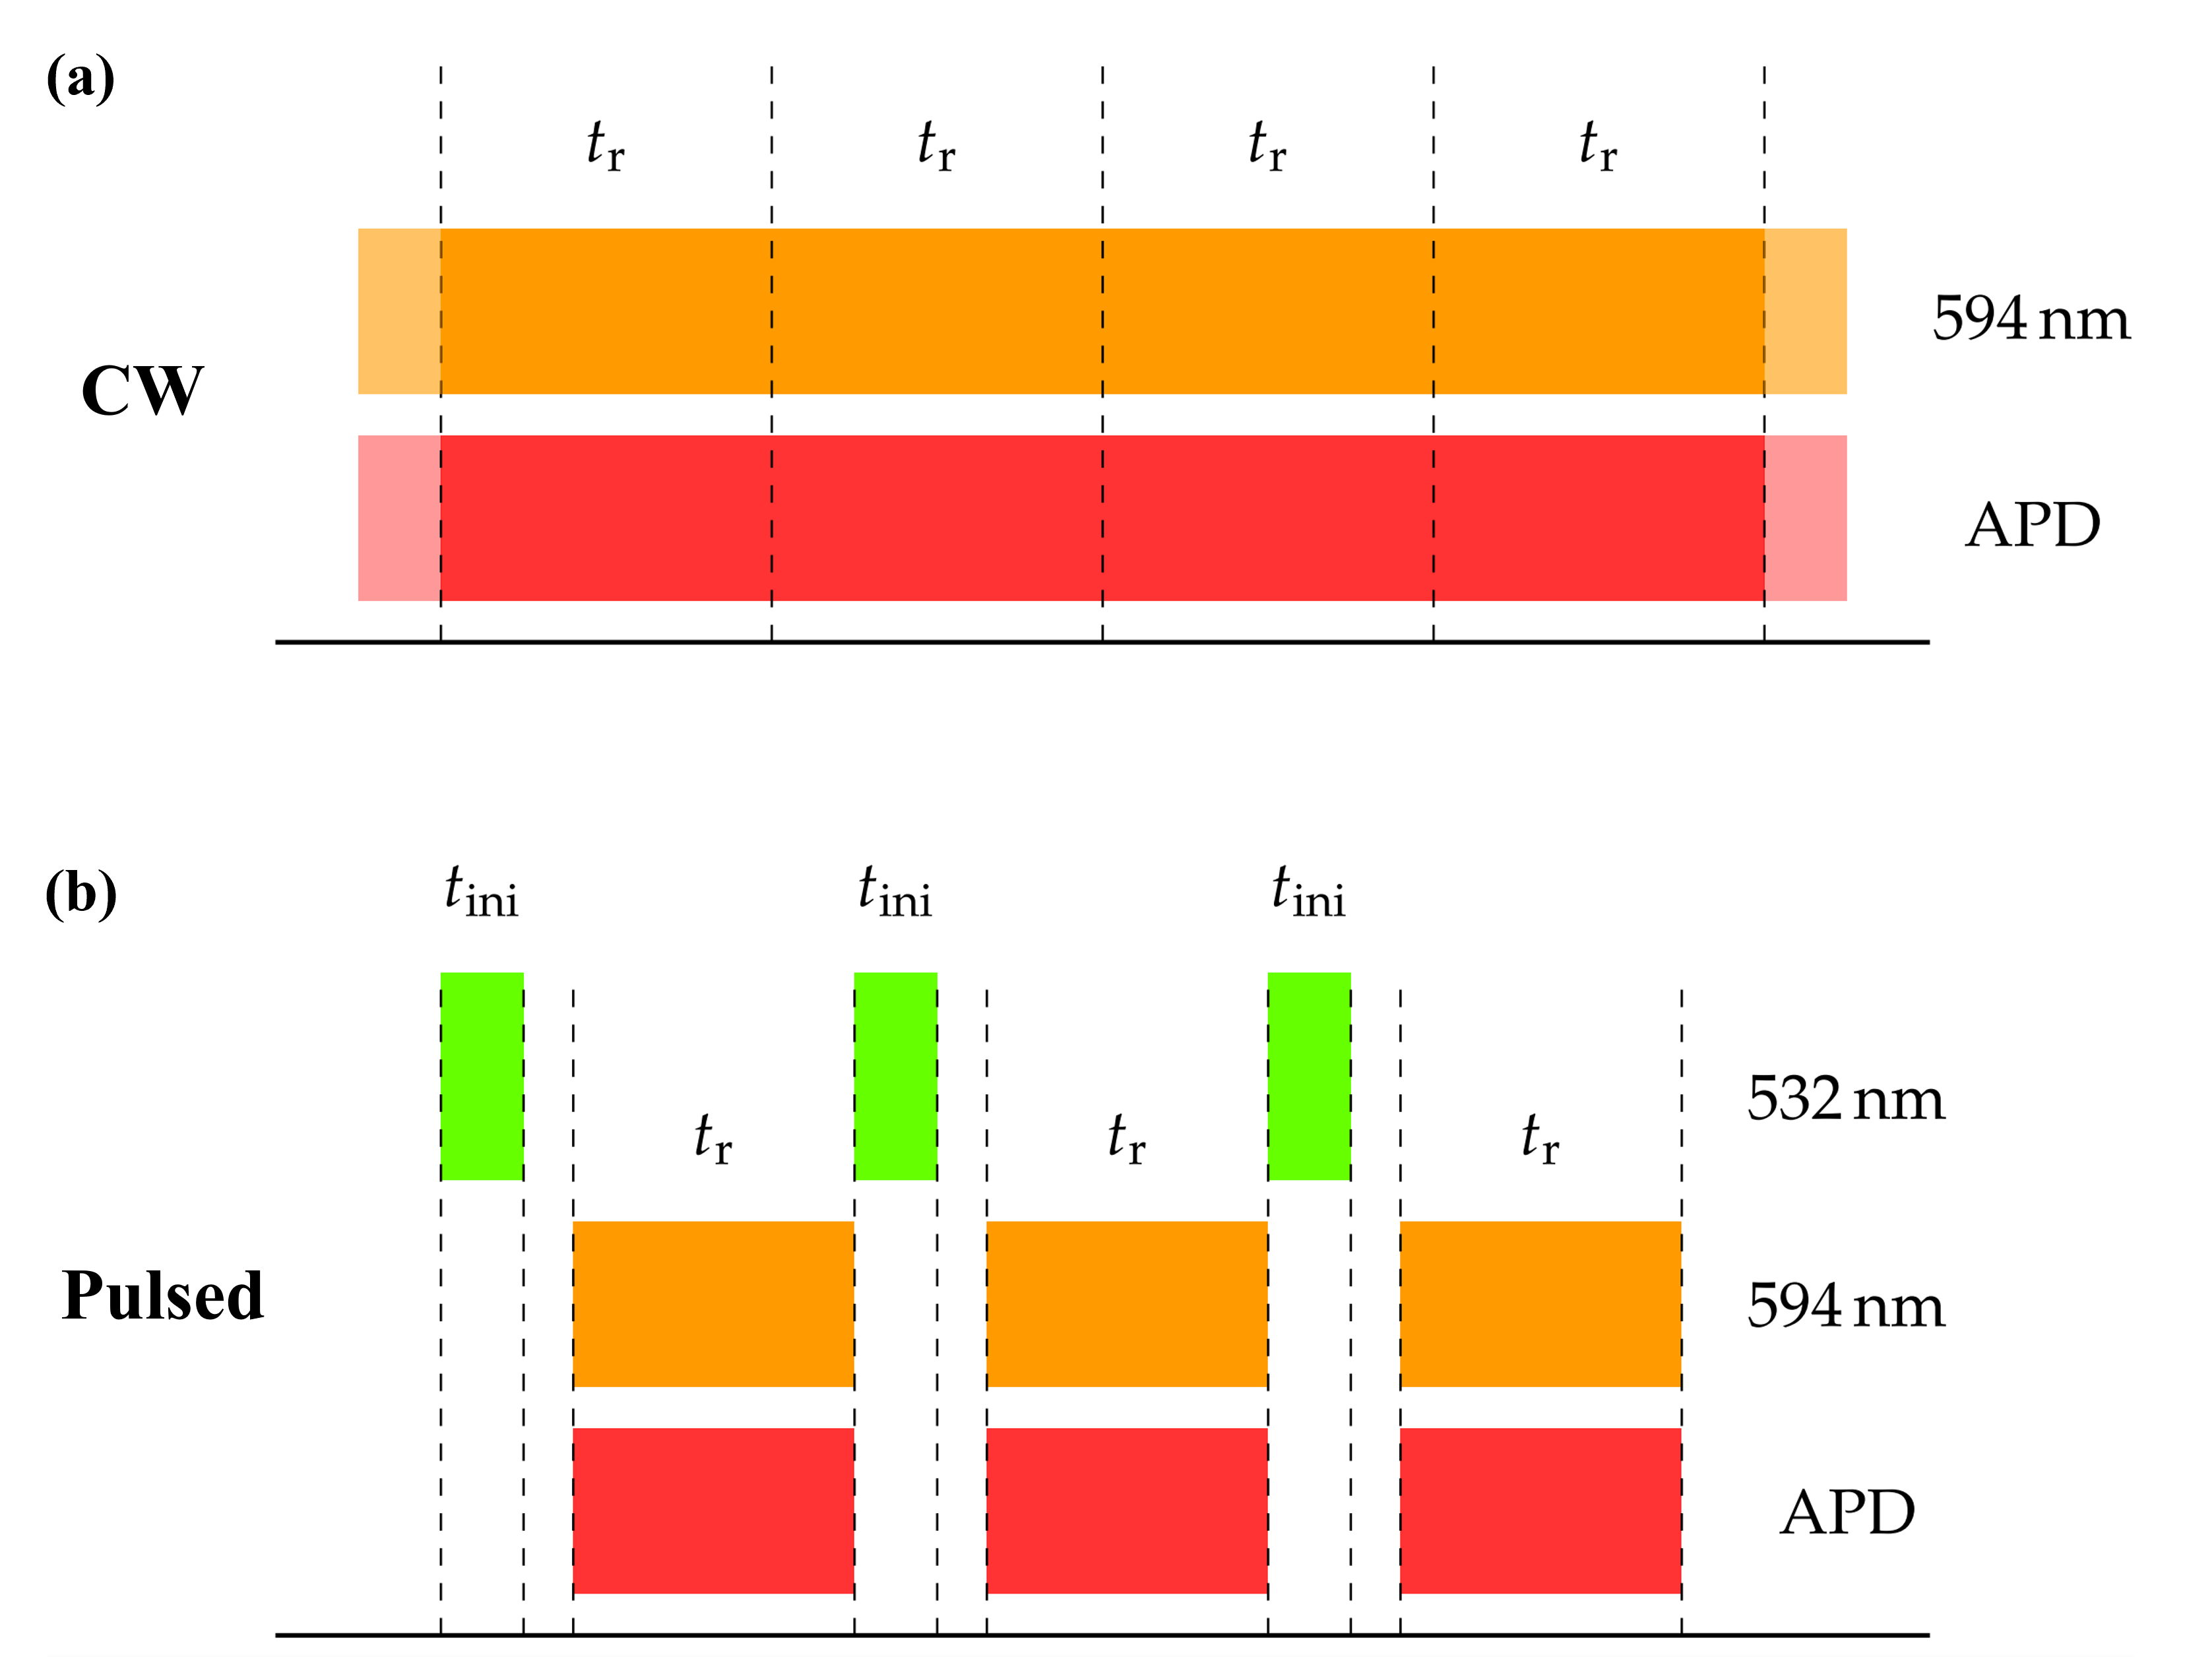
\includegraphics[width=1.0\textwidth]{figures/Chapter 2/Measurement Sequence.png}
  \caption[CW和Pulsed测量序列简图]{CW和Pulsed测量序列简图,$t_r$为读出时间窗口,$t_{ini}$为初始化时间长度。}
  \label{fig: Measurement Sequence}
\end{figure}

对于(a)图中CW序列而言,在每一轮10 $s$的测试过程中,594 nm的橙光持续保持开启的状态。由于AOM的开启存在上升沿和稳定性的问题,每次TT计数器的触发接口在开启橙光后10 $\mu s$后,施加一个50 $ns$的高电平脉冲,使计数器启动。随后TT计数器的测量脉冲序列通道保持10 $s$的高电平状态,在这个过程中,TT以10 $\mu s$为时间分辨率窗口进行持续地记录数据。序列结束的时候,保持橙光持续开启2 $\mu s$,以确保测量序列末端的光强稳定。因为是连续测量,所以在设置不同的读出时间$t_r$的时候,只需要通过不同数量的相邻time bins进行合并,即可得到不同的$t_r$,即$t_r = n_{merge} \times 10\ \mu s$,在这个过程中我们是依次递推合并相邻的time bins。例如我们想要读出时间为$t_r = 1\ ms=100 \times 0.1\ \mu s$,这个时候$n_{merge} = 100$,我们就合并0-99号、1-100号、2-101号等等这些time bins,以此类推,从而使得有限的数据最大程度的被利用起来。然后将结果归一化,利用$Python$中的$Matplotlib$包绘制以对数坐标为纵轴概率,以每个$t_r$内的光子数为横轴事件的概率分布直方图。

对于(b)图中的Pulsed序列而言,每次用532 nm的绿光初始化序列长度为$t_{ini} = 3\ \mu s$,随后有一段长为$t_{wait} = 1\ \mu s$的间隔,使电荷态充分转换并稳定,最后是利用 594 nm的橙光进行读出,TT计数器也同时启动,记录APD接受光子生成的脉冲序列。数据后处理和绘图的方式和CW序列相同。

在数据拟合的过程中,我们应用了$SciPy$中的“$curve\_fit$”函数,根据第二章中的理论模型,拟合出最合适的参数,并确定拟合的标准差(Standard Deviation,STD)。同时通过改变$n_{merge}$的值来改变$t_r$,使得最后的STD尽可能的小。$t_r$过大的时候,大量的time bins合并在一起,使数据的密度过大,从而难以得到合理的分布规律;而较小的$t_r$会使得数据的密度过小,可能出现的情况较少,可用于拟合的数据点不足,难以得到合理的拟合结果。

 
\end{document}
\end{document}